\section{Numerical Analysis of Complex LSF Walls-Ambient Conditions}

Finite element method (FEM) is a numerical technique to arrive at a solution for a boundary value problem using partial differential equation to the nearest approximation. The analysis carried out with this methodology is termed as Finite Element Analysis (FEA). FEA works with the logic of minimising the error function in the given boundary value problem by employing variations methods from calculus. Many numerical validation methods prevail till date, but FEM is one of the easiest methods of solving the given problem. The major advantages of using FEM is that any complex problem can be discretised into a simpler problem and analysed in parts to arrive at the result. 

There are many FEA packages commercially available in the market. Packages that are widely used by researchers and engineers are ANSYS, ABAQUS, NASTRAN, PATRAN, LS-Dyna etc. Each package has its own unique features and varies in their utility with respect to time and release of the software patches. The decision to use a specific FEA package depends on the necessity of the end user. ABAQUS is proposed for use in this research for structural FE analysis. ABAQUS originally got its name from the calculation tool abacus. Major modules of the software are CAE (Complete ABAQUS environment), explicit, standard, CFD (Computational Fluid Mechanics) and Electromagnetic. The CAE module is generally used to develop the models in a GUI (Graphical user interface) environment. Other methods of importing the model from other FEA packages are also readily available. Programming languages such as Fortran and Python are embedded within the ABAQUS environment so that the end user is left with endless customization options depending upon their requirement. The standard module in the ABAQUS is used for addressing problems related with general structural and multiphysics. As the name suggests the explicit module addresses the contact problems in an efficient manner. The CFD module is used for computational fluid dynamics problems involving liquid flow or thermal flow problems and the Electromagnetic environment is meant for problems related to computational electromagnetics. Since the research focuses is on the structural behaviour of LSF walls CAE module will be used for numerical modelling and analysis.

\section{ABAQUS Modelling Set-up}

The numerical models were created in ABAQUS within the CAE environment. Despite the ambient capacity experiments consisting of 4 and 6 studs the numerical models were created with single set of studs only to achieve maximum computational efficiency. As the stud arrangements are symmetric in the ambient temperature capacity tests, modelling and analysing the single set of studs was considered as the efficient approach. This consideration was based on past literature from the FE structural models developed by \citet{Shahbazian2011,Gunalan2013f,Kesawan2016a,Ariyanayagam2019}. The FEA simulation for predicting the ambient temperature capacity of double and staggered stud walls comprises of two steps. Firstly, linear buckling analysis was performed on the studs to determine the buckling load under ambient conditions. After determining the buckling load, local imperfections were included in the model (d/150) based on past literature by \citet{Gunalan2013f} and static non-linear analysis was carried out to determine the ultimate capacity of the studs. The following steps were carried out to determine the buckling load of the studs. As ABAQUS does not have any system of units built in, it is left to the discretion of the user to follow consistent units throughout the model. The International System of Units (SI) was used throughout the modelling and analysis of the complex LSF walls in this research study. The first step was to create the sketch of the studs in the GUI windows as shown in \Cref{fig:ABAQUS-sketch}.
\begin{figure}[!htbp]
	\centering
			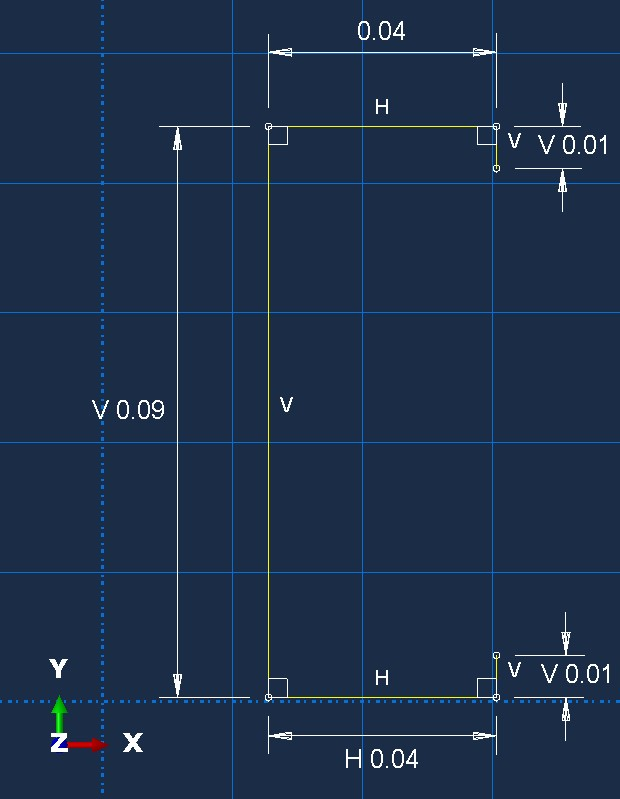
\includegraphics[scale=0.4]{ABAQUS-sketch.jpg}\\
		\caption{Input screen for sketching showing typical LCS - ABAQUS }
		\label{fig:ABAQUS-sketch}
\end{figure}

Centreline dimensions were followed for the modelling as shell modelling technique was used for the simulation. 3D shell elements were used for the linear buckling and static non-linear analysis under ambient temperature conditions using S4R (4-node shell) element with reduced integration. After completing the section sketch, the model was extruded to 3 m length, depicting studs in the experimental set-up. The extruded section sketch forms a FEATURE in the FE model. The FEATURE forms the PART with additional components and are discussed next. It is to note that, a PART can have single or multiple FEATURES. Some of the additional components of a PART includes, SETS, Section Assignments and Engineering Features such as Inertia and Spring Constants. However, only SETS and Section Assignment will be used in the current structural FE model. For FEA the material properties plays a major role in determining the structural capacity of the developed model. The material properties of steel such as yield stress and elastic modulus were extracted from \citet{Kankanamge2011} which was later confirmed by \citet{Rokilan2019}. The measured yield strength and elastic modulus are entered in the true stress-strain form as Engineering stress-strain curves are not accepted form of input in the ABAQUS CAE environment. Yield strength value of 610 MPa and elastic modulus of 200 GPa was used for the ambient temperature structural analysis. The density of steel was kept constant at 7850 $kg/m^3$. Once the material properties of steel are keyed in, it is assigned to the corresponding PART through Section Assignment. The PART is then imported into the assembly, wherein two independent INSTANCES of the stud is created. Multiple point constraints (MPC's) using beam element was used at the top and bottom of the model on a reference point replicating the centre of gravity (CG) of the model and appropriate boundary conditions were assigned to it. This is achieved by tying all the edges at the top and bottom of the model to their corresponding reference points as shown in \Cref{subfig:abaqus-mpc-contraint}. Translations along the x, y and z-axes were fixed at the bottom of the model while the model was free to move along the z-axis at the top. The model was fixed against rotation along the z-axis only at the top and bottom. Translation along the x-axis was fixed on the stud flanges at screw locations (300 mm) to simulate the lateral restraints provided by plasterboards on the exterior flanges. Individual plasterboards were not modelled to improve the computational efficiency. Lateral restraints provided by the noggings were specified at 1 m intervals on all the flanges. A mesh density of 4 mm was adopted throughout the model based on past literature and initial sensitivity study as shown in \Cref{subfig:abaqus-meshes-structural}. A concentric unit load was applied at the top reference point and the buckling analysis was carried out by specifying linear perturbation in the step option. \Cref{fig:abaqus-full-assembly} shows a typical double stud wall model in ABAQUS. Ten eigen modes were requested for each model to investigate the buckling modes of the studs. The input file was modified with ``*NODE FILE U" argument to collect the buckling modes as a data file and to be used in the non-linear analysis. The buckling analysis results are viewed with the in-built data visualization tool in ABAQUS CAE environment.
\begin{figure}[!htbp]
	\centering
	\begin{subfigure}[b]{0.4\textwidth}
		\centering
		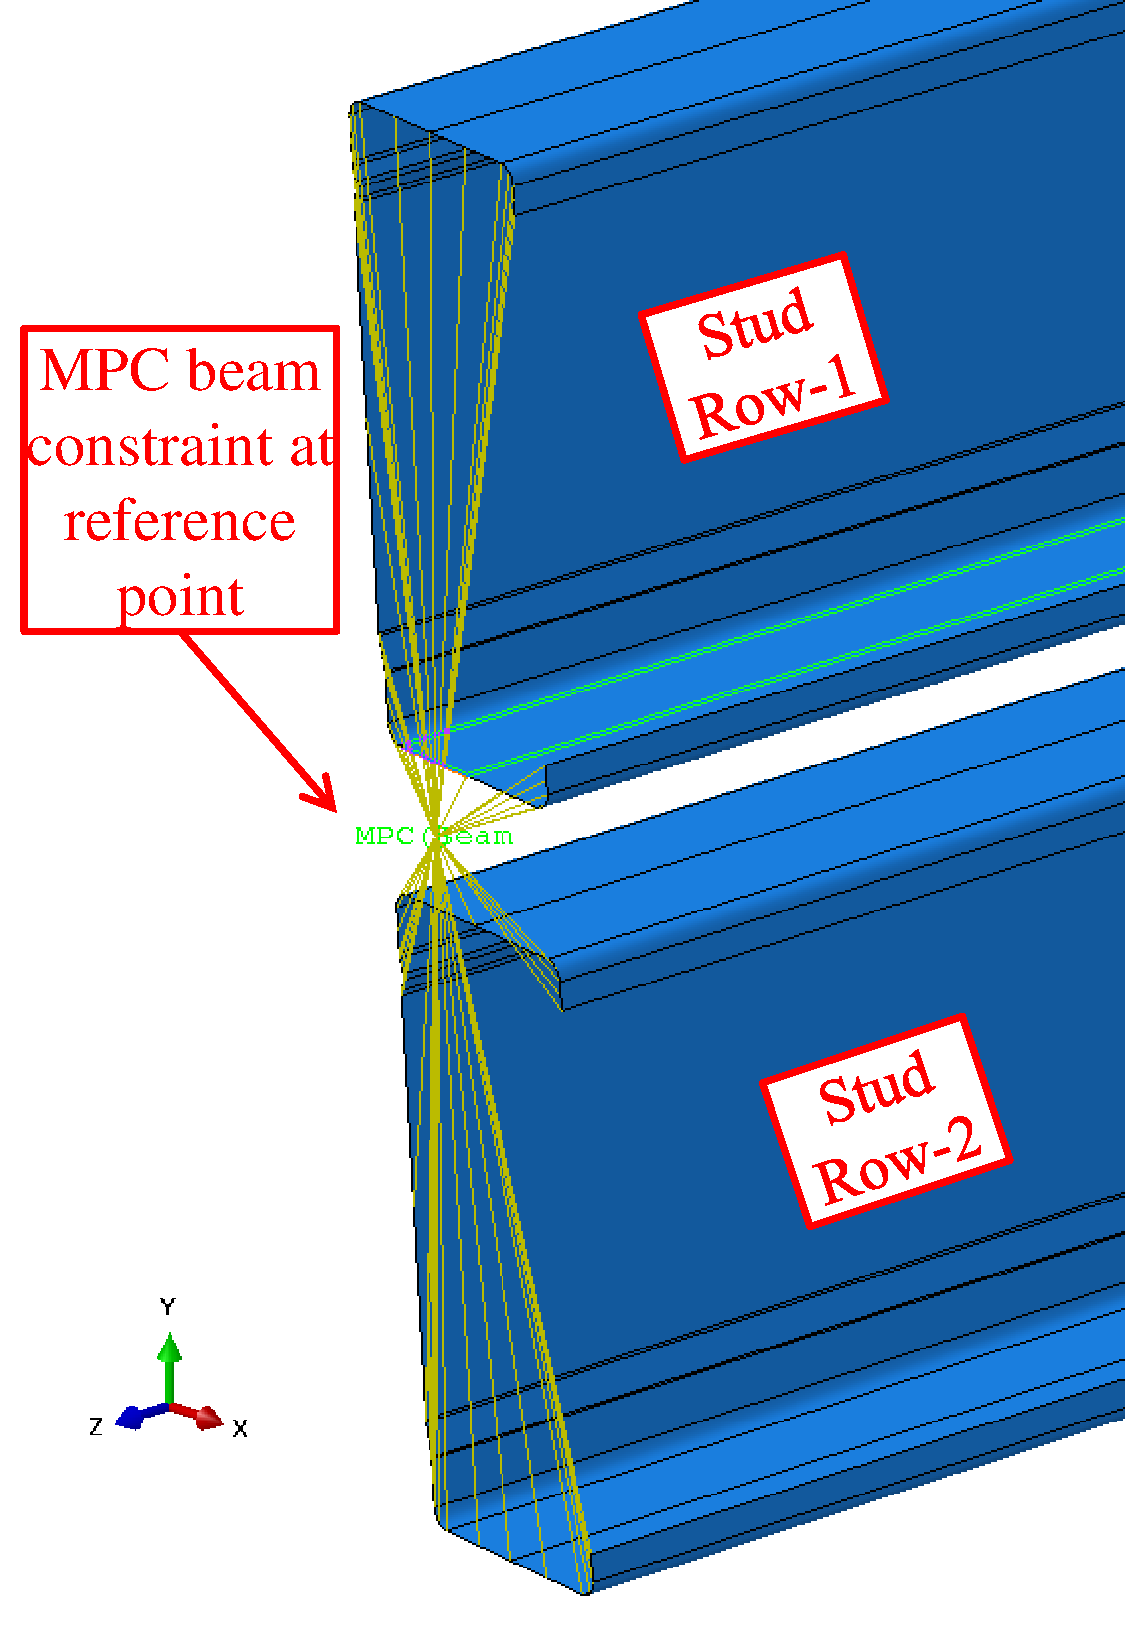
\includegraphics[width=\textwidth]{abaqus-mpc-contraint.pdf}
		\caption{}
		\label{subfig:abaqus-mpc-contraint}
	\end{subfigure}
	\begin{subfigure}[b]{0.4\textwidth}
		\centering
		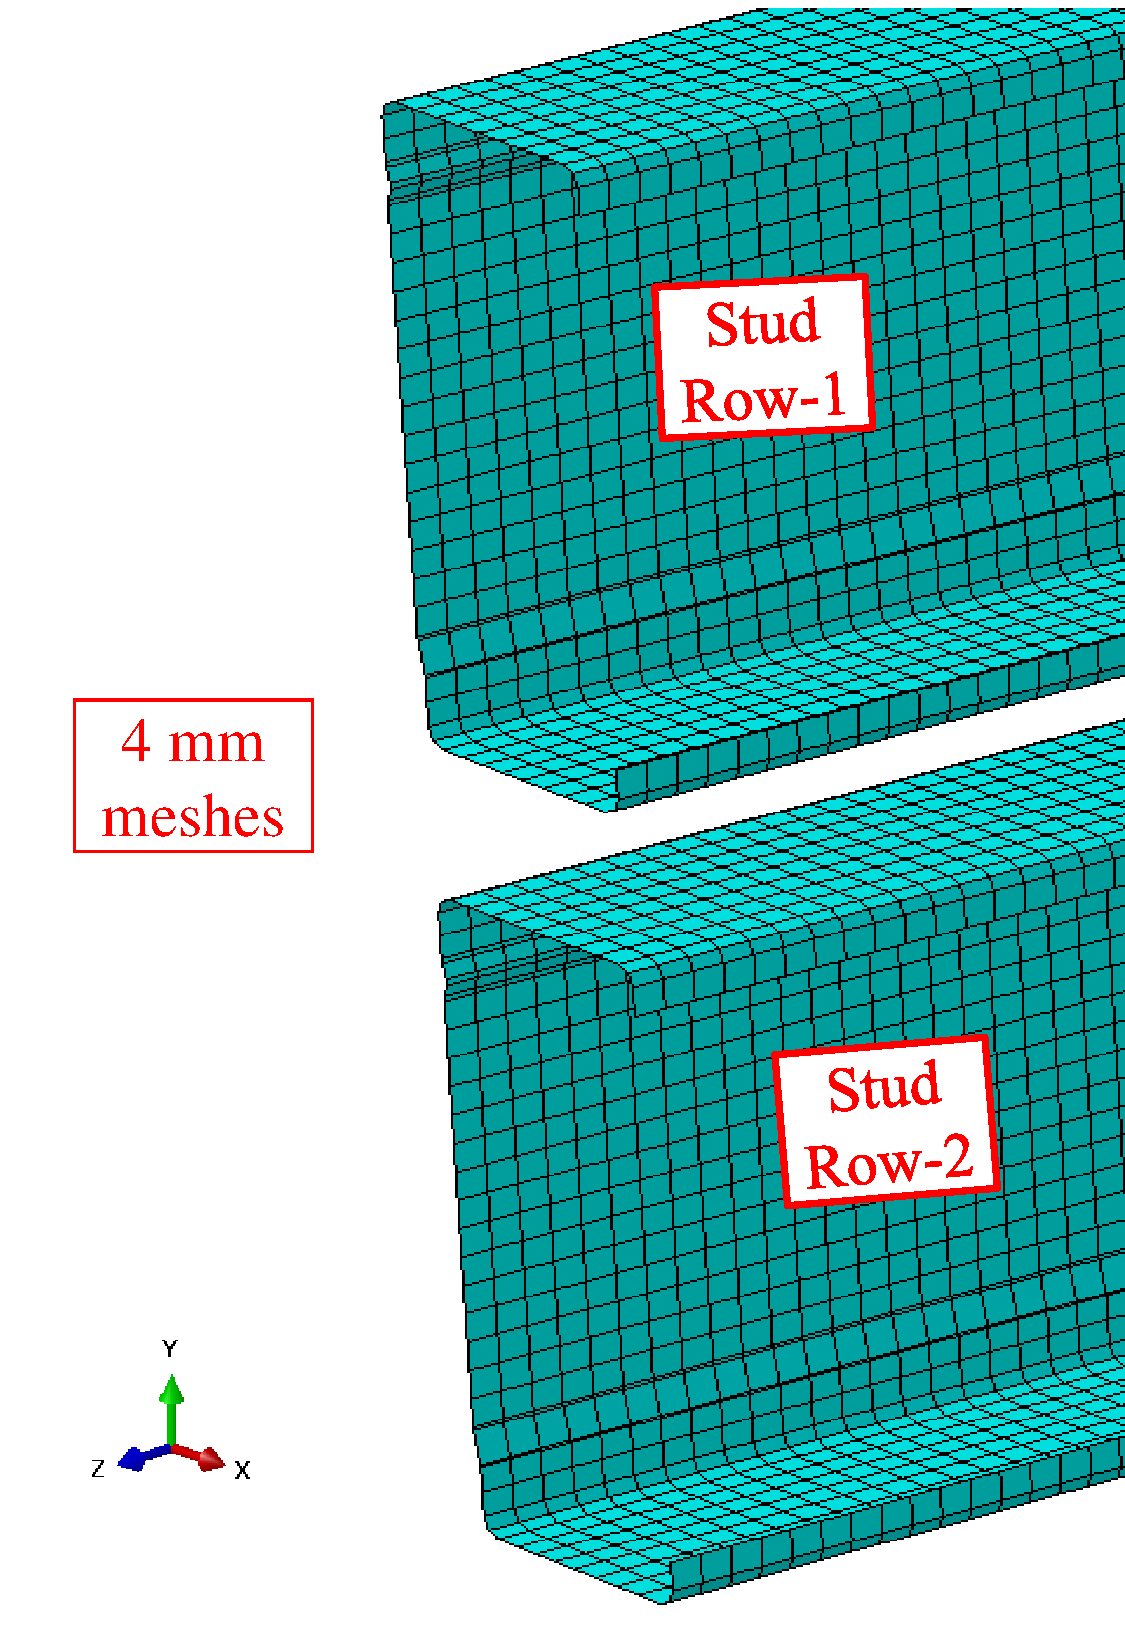
\includegraphics[width=\textwidth]{abaqus-meshes-structural.pdf}
		\caption{}
		\label{subfig:abaqus-meshes-structural}
	\end{subfigure}
	   \caption{Typical double stud model assembly in ABAQUS}
	   \label{fig:abaqus-typical-model}
\end{figure}
\begin{figure}[!htbp]
	\centering
			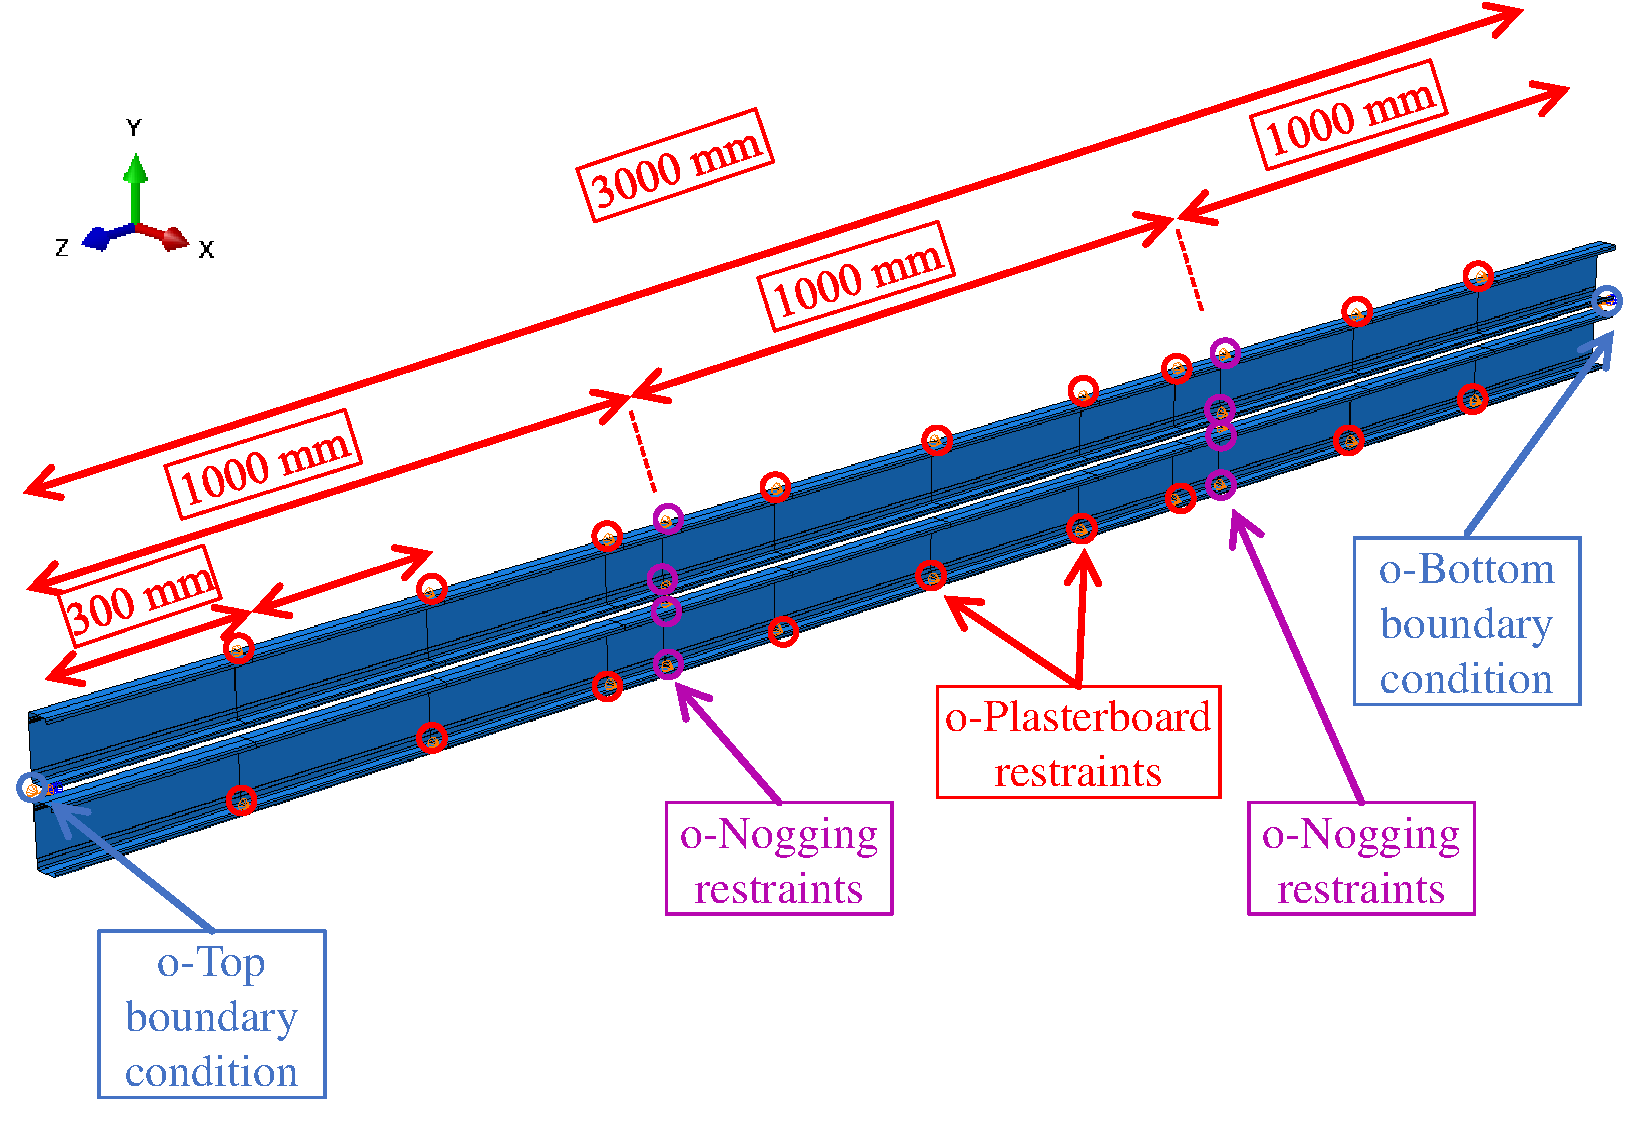
\includegraphics[scale=0.5]{abaqus-assembly-structural.pdf}\\
		\caption{Full assembly of double stud LSF wall in ABAQUS}
		\label{fig:abaqus-full-assembly}
\end{figure}

The second step is to conduct non-linear structural analysis and to determine the ultimate load carrying capacity of the studs. The model used for the buckling analysis is imported to a new file to conduct the analysis. The analysis step option is replaced with static general option and the ``Nlgeom" feature is turned to include the nonlinear effects as a result of large deformation in the model. Maximum incrementation needed for the analysis are specified depending on the model and also the initial, minimum and maximum increment size. Specific dissipated energy fraction is used for automatic stabilization in the model for better convergence. History output requests are specified at the top reference point to monitor the axial displacement and at the bottom reference point to monitor support reactions throughout the analysis. These history outputs are stored in the output database (ODB) file for every n\(^{th}\) increment in the analysis. Maximum principle stresses in all the elements throughout the model was also extracted from the analysis. Structural model validation and comparison with the experimental results are discussed next.

\section{Structural Model Prediction - Ambient Temperature Capacity Tests}

Structural FE models were developed for all the tested LSF wall configurations listed in \Cref{ch:Ambient}. This includes wall configurations such and single and double stud LSF walls. The axial displacement versus load results from the developed structural FE models are detailed and compared with the experimental results and are discussed next.  

\subsection*{Test-AT1}

Test-AT1 was conducted on double stud LSF wall with 90 mm deep. 0.95 mm thick studs as shown in \Cref{fig:AT1-plan-fea}. The applied axial load versus displacement results from FEA and experiments are shown in \Cref{fig:AT1-fea-results}. FE structural analysis for Test-AT1 resulted a maximum axial compression capacity of 71.97 kN while it was 73.0 kN from the experimental results which is 1.03 kN less than the experimental results. Slope exhibited by the load versus axial displacement curve from FE structural analysis was steep in comparison with the experimental results.     
\begin{figure}[!htbp]
	\centering
			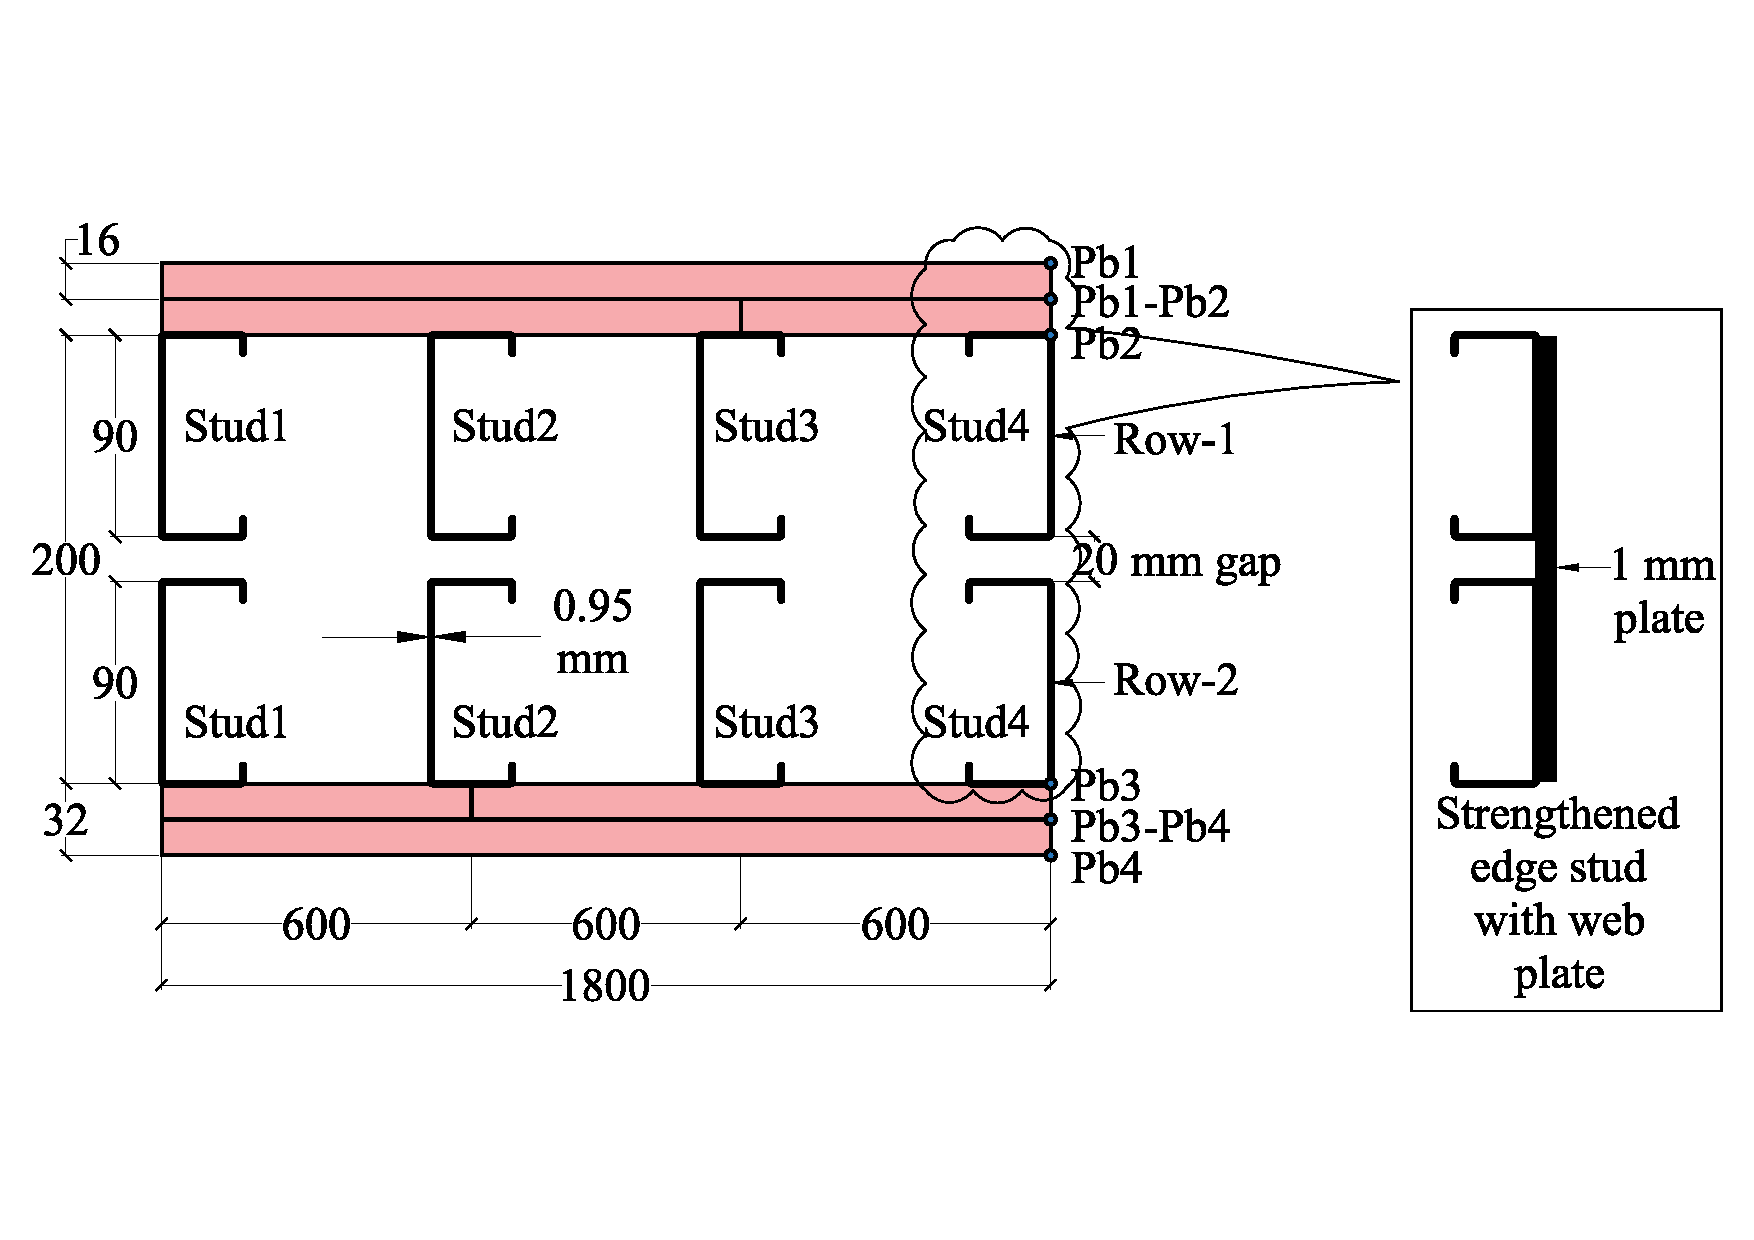
\includegraphics[scale=0.2]{AT1-plan.pdf}\\
		\caption{Test-AT1 plan}
		\label{fig:AT1-plan-fea}
\end{figure}
\begin{figure}[!htbp]
	\centering
			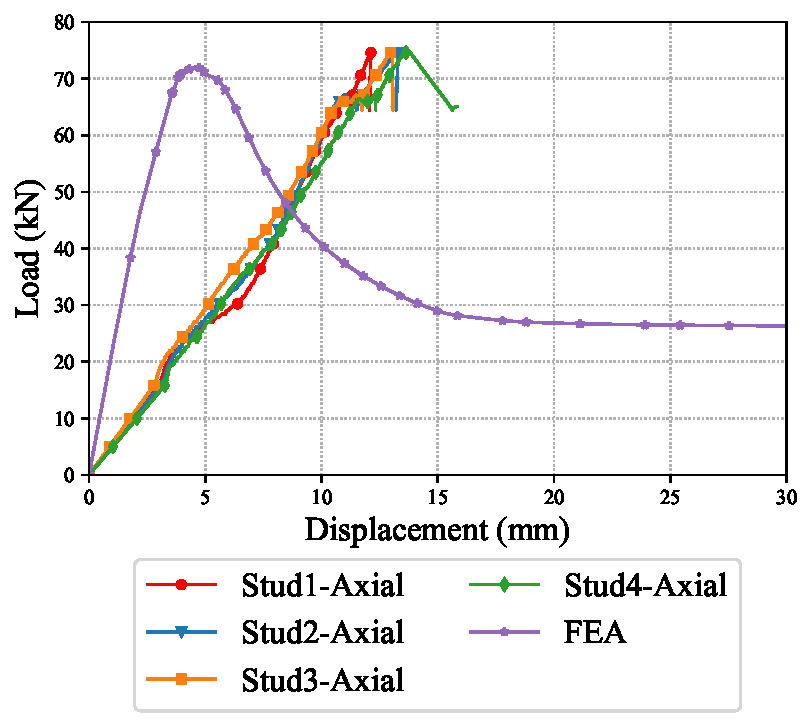
\includegraphics[scale=0.6]{AT1-Load-Axial-Exp-vs-FE.pdf}\\
		\caption{Test-AT1 FEA and experimental results comparison - Applied load versus axial displacement}
		\label{fig:AT1-fea-results}
\end{figure}
\begin{figure}[!htbp]
	\centering
	\begin{subfigure}[b]{0.4\textwidth}
		\centering
		\includegraphics[width=\textwidth]{AT1-buckling-FEA.pdf}
		\caption{}
		\label{subfig:AT1-buckling-FEA}
	\end{subfigure}
	\begin{subfigure}[b]{0.4\textwidth}
		\centering
		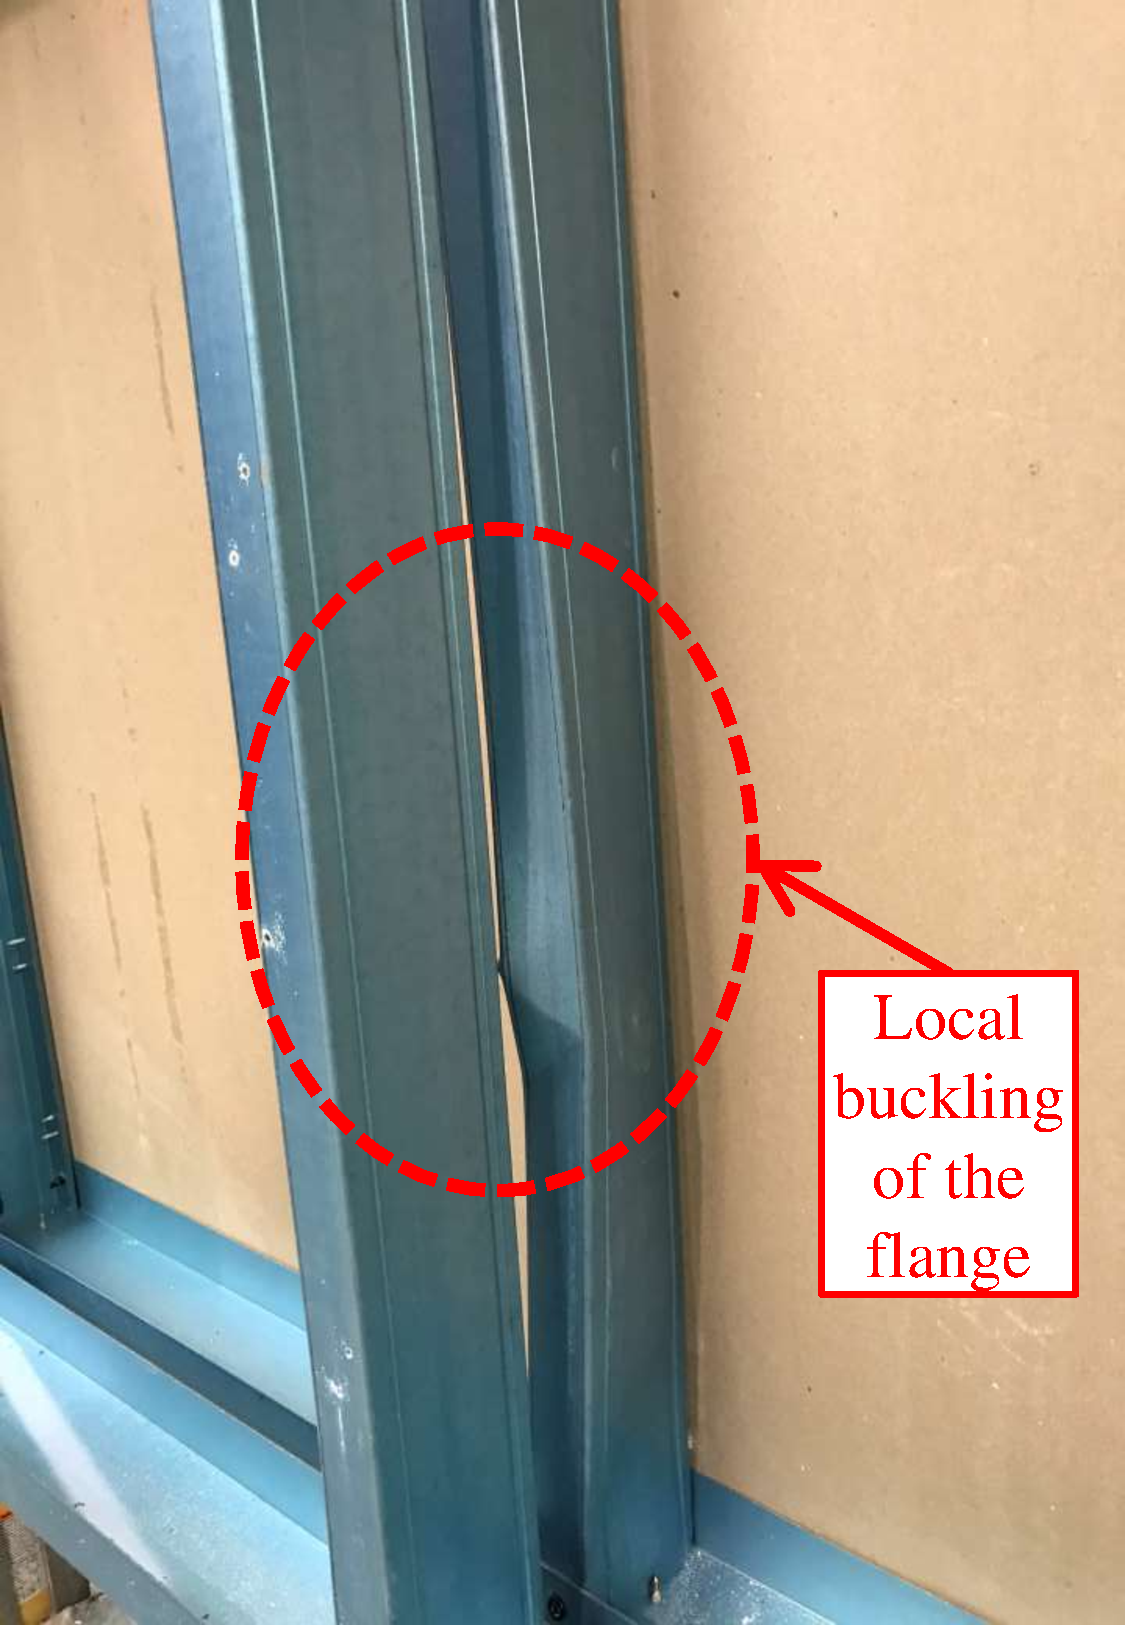
\includegraphics[width=\textwidth]{AT1-buckling.pdf}
		\caption{}
		\label{subfig:AT1-buckling-experiment}
	\end{subfigure}
	   \caption{Test-AT1 - Buckling of studs (a) FEA (b) Experiment}
	   \label{fig:AT1-buckling-fea-comparison}
\end{figure} 

As general static method of analysis is adopted in FE structural analysis the axial load is applied instantaneously by load control technique. This results in a sudden increase in the initial load given to the model. Although the increment to achieve the maximum load is smaller the analysis tends to apply the load instantaneously to the model causing the difference in slope of the load versus axial displacement curve in comparison with the experiments. The lateral deflections from the FEA are not considered for comparison as local buckling was the dominant mode of failure in studs. Failure modes predicted from the FE analysis is also compared with the experimental results and is shown in \Cref{fig:AT1-buckling-fea-comparison}. Buckling of the stud flanges from the experiments could also be captured by the developed FE model.

\subsection*{Test-AT2}

Ambient capacity Test-AT2 was also conducted on double stud LSF walls with 90mm deep studs. However, the stud thickness was 0.75 mm as shown in \Cref{fig:AT2-plan-fea}. The structural FE model resulted an axial compression capacity of 46.25 kN while the experiment resulted an axial compression capacity of 47.08 kN as shown in \Cref{fig:AT2-fea-results}. The ambient temperature compression capacity predicted by the structural FE model was 0.83 kN less than the experimental results. The local compressive failure of the stud flanges showing a dimple in \Cref{subfig:AT2-buckling} could also be simulated by the developed FE model as shown in \Cref{subfig:AT2-buckling-FEA}. 
\begin{figure}[!htbp]
	\centering
			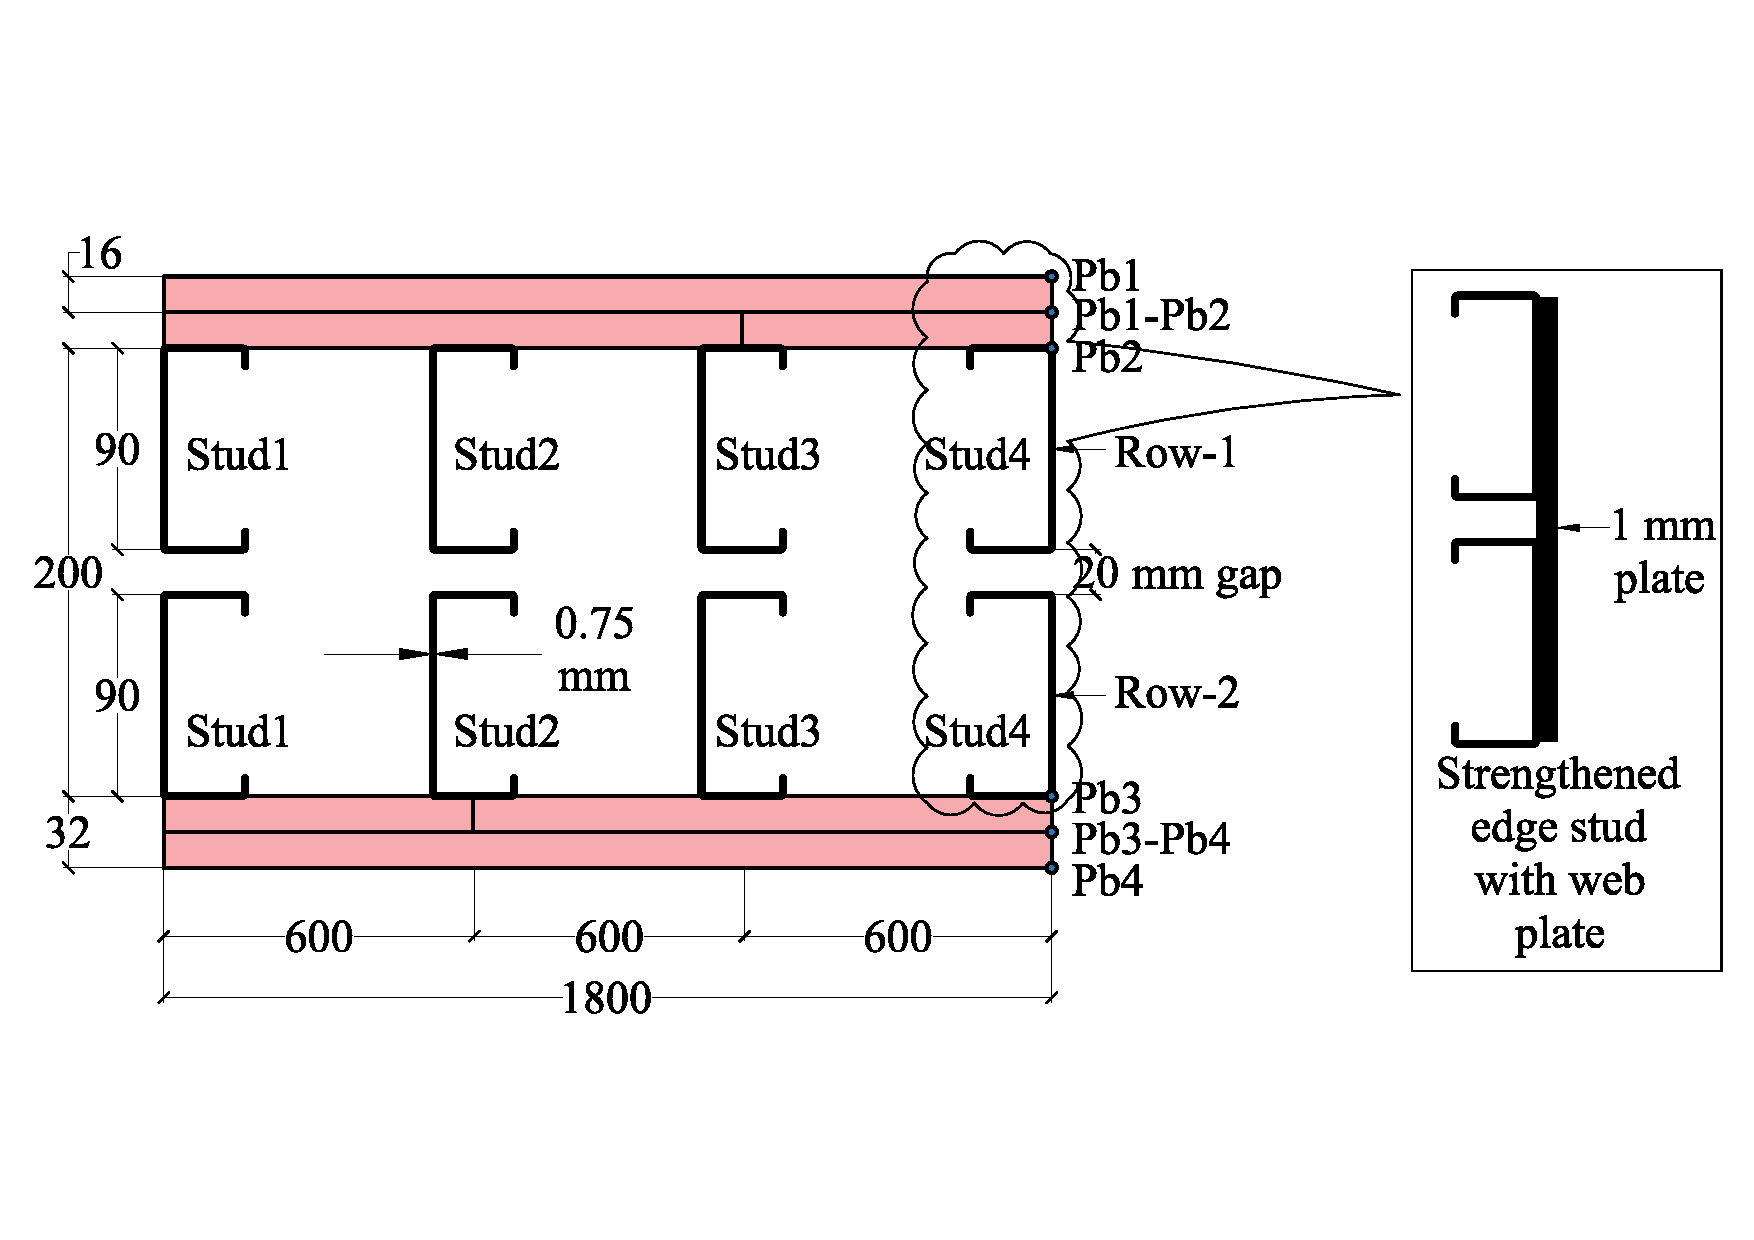
\includegraphics[scale=0.25]{AT2-plan.pdf}\\
		\caption{Test-AT2 plan}
		\label{fig:AT2-plan-fea}
\end{figure}
\begin{figure}[!htbp]
	\centering
			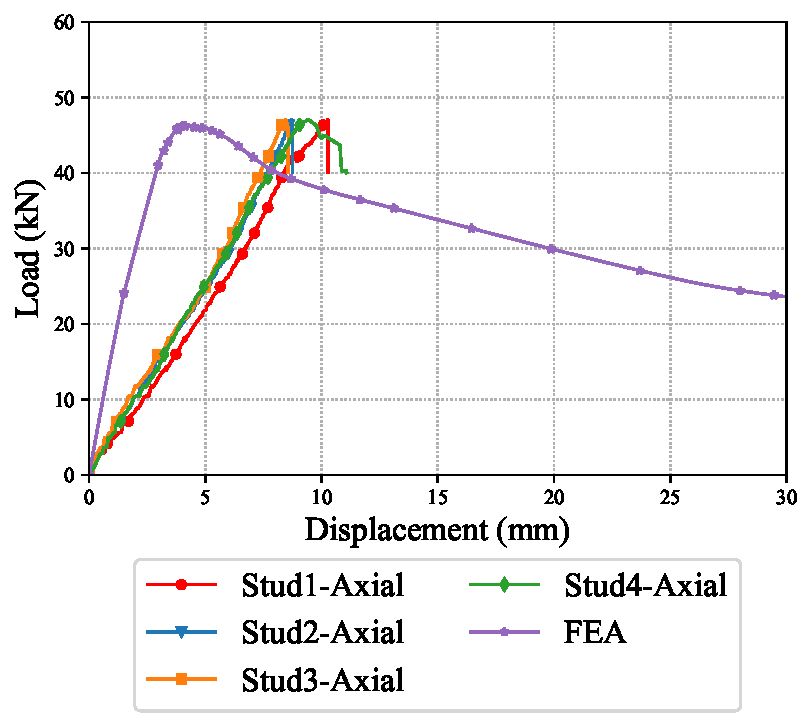
\includegraphics[scale=0.6]{AT2-Load-Axial-Exp-vs-FE.pdf}\\
		\caption{Test-AT1 FEA and experimental results comparison - Applied load versus axial displacement}
		\label{fig:AT2-fea-results}
\end{figure}
\begin{figure}[!htbp]
	\centering
	\begin{subfigure}[b]{0.4\textwidth}
		\centering
		\includegraphics[width=\textwidth]{AT2-buckling-FEA.pdf}
		\caption{}
		\label{subfig:AT2-buckling-FEA}
	\end{subfigure}
	\begin{subfigure}[b]{0.4\textwidth}
		\centering
		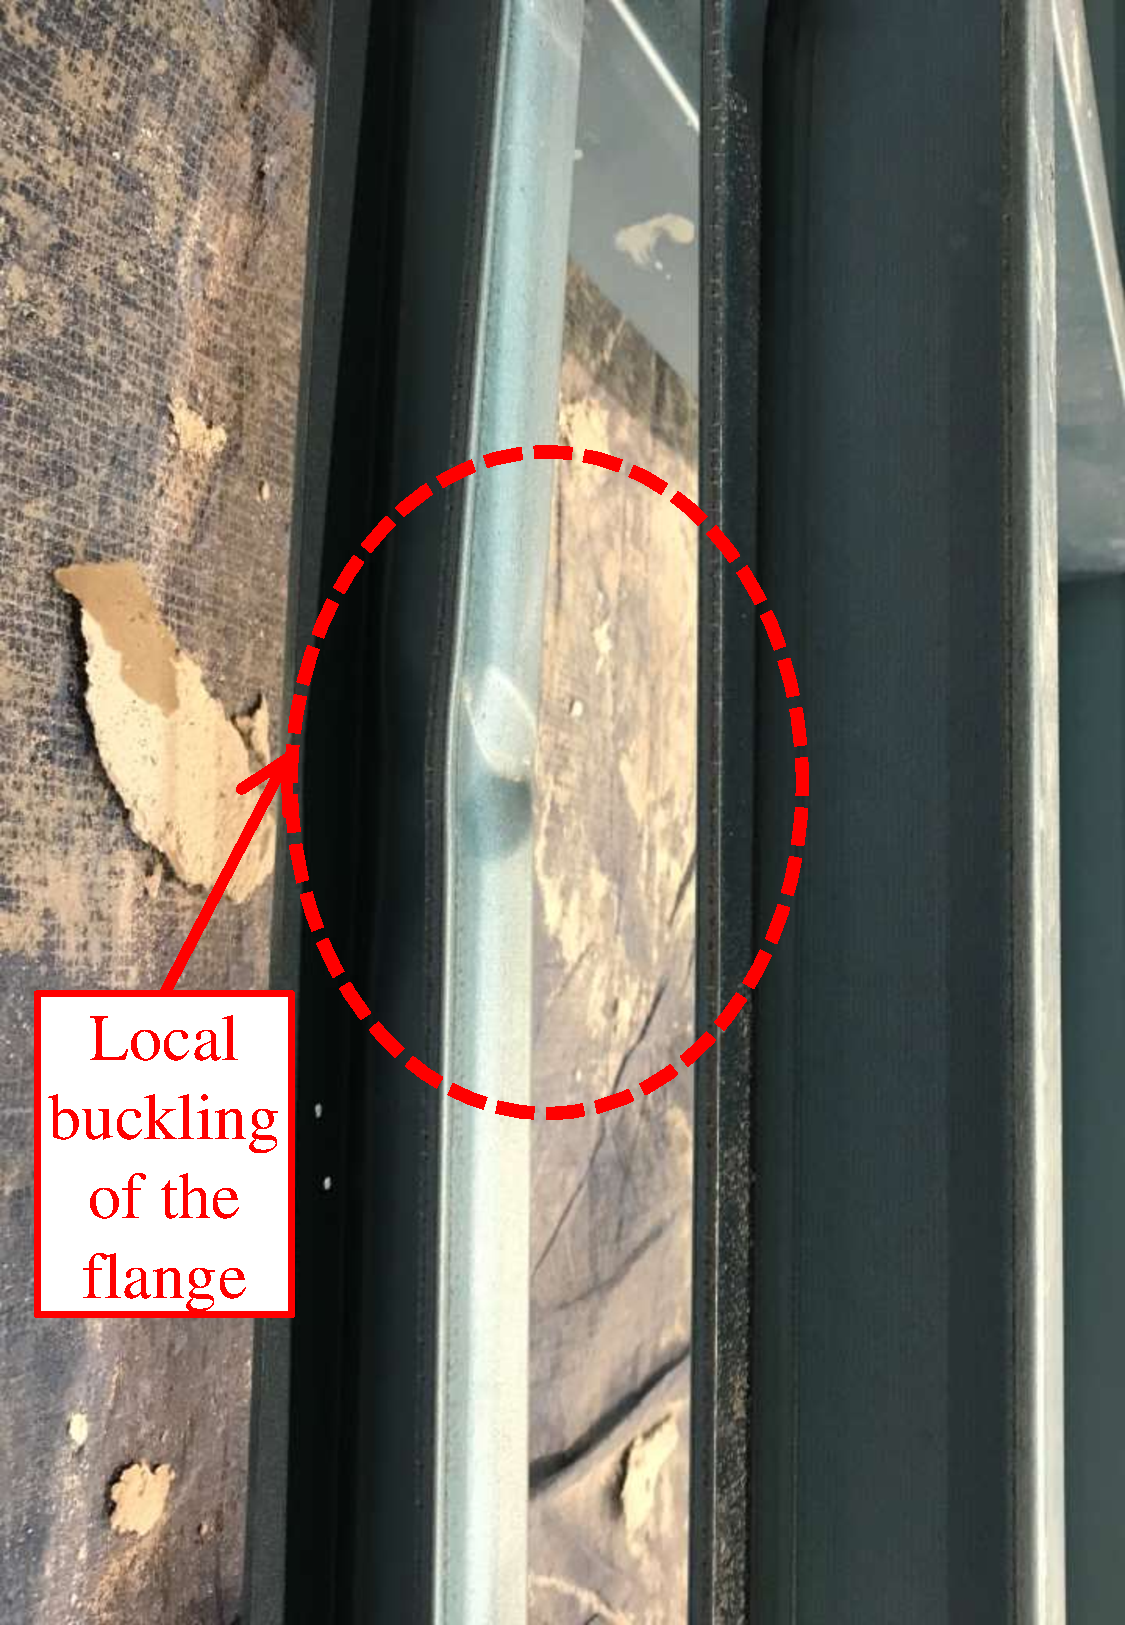
\includegraphics[width=\textwidth]{AT2-buckling.pdf}
		\caption{}
		\label{subfig:AT2-buckling-experiment}
	\end{subfigure}
	   \caption{Test-AT2 - Buckling of studs (a) FEA (b) Experiment}
	   \label{fig:AT2-buckling-fea-comparison}
\end{figure} 

It is to note that, the experimental investigation under ambient temperature conditions were conducted on LSF walls with either for or six stud arrangements. However, in the developed structural FE models single stud row was used for computational efficiency. Therefore, the ambient temperature capacity results of Test-AT2 and AT3 were compared with the same structural FE model. As discussed in \Cref{ch:Ambient}, \Cref{sec:AT3} the influence of effective plasterboard restraints to the stud flanges is not considered in the present FE model. It was assumed that the plasterboards provide full minor axis restraints to the stud flanges during the structural model simulation. This assumption holds good as global buckling was not the dominant failure mode in the double stud wall ambient temperature capacity tests.

\subsection*{Test-AT3}

\Cref{fig:AT3-fea} shows the comparison between the ambient temperature capacity versus displacement predictions from FE structural model against the experimental results. As stated earlier Test-AT3 was conducted with six studs unlike four studs in Test-AT2 as shown in \Cref{fig:AT3-plan-fea}. The experiment results gave an ambient temperature compression capacity of 39.42 kN. The FE structural models prediction was 46.25 kN which is 6.83 kN greater than the experimental results. However, as stated earlier in \Cref{ch:Ambient}, \Cref{sec:AT3} the reduction in axial capacity test results was attributed by the weak plasterboard minor axis restraints provided to the end studs. The local crushing failure experienced by the end stud in experimental investigation could also be predicted by the developed FE model as shown in \Cref{fig:AT3-buckling-fea-comparison}. The crushing failure shown in \Cref{subfig:AT3-buckling-FEA} and the local buckling failure shown in \Cref{subfig:AT2-buckling-FEA} corresponding to Test-AT2 were predicted by the same structural FE model. 
\begin{figure}[!htbp]
	\centering
			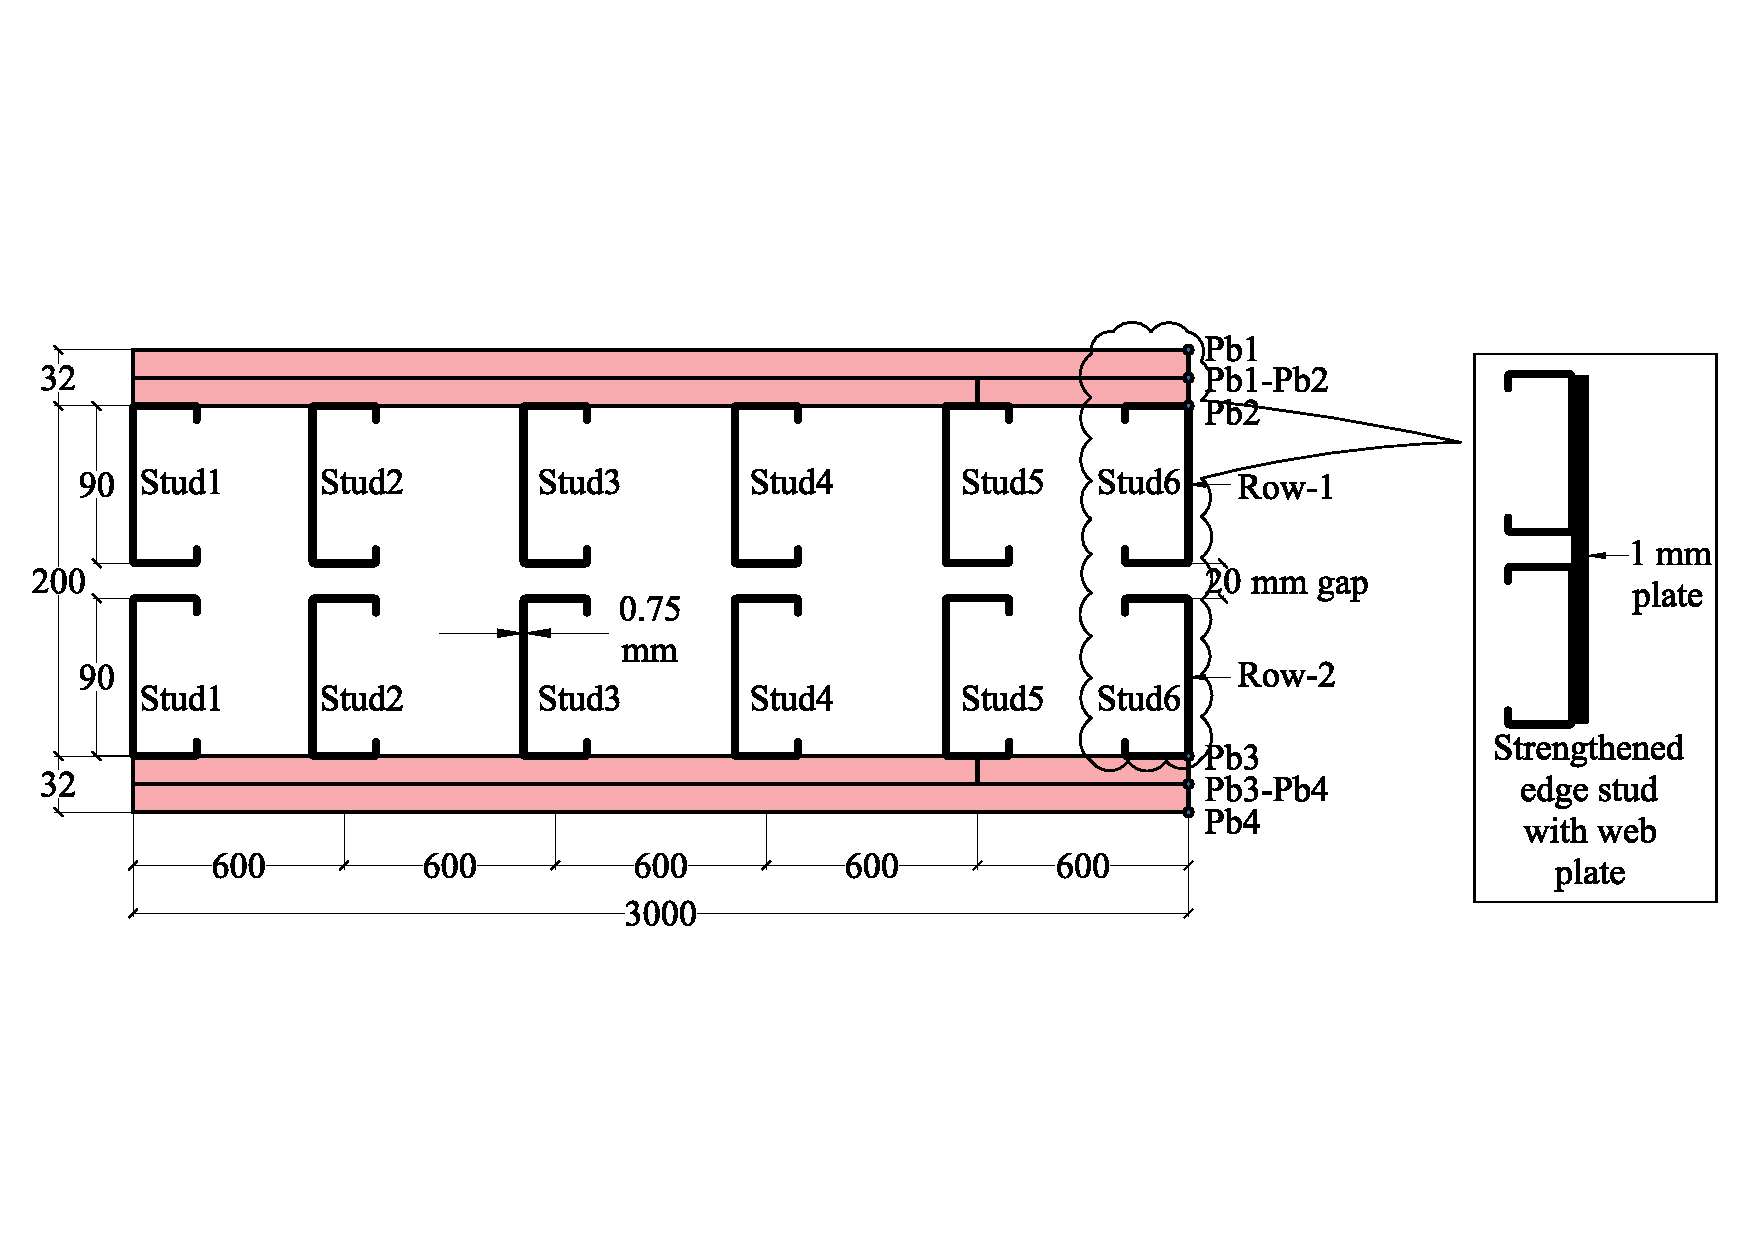
\includegraphics[scale=0.25]{AT3-plan.pdf}\\
		\caption{Test-AT3 plan}
		\label{fig:AT3-plan-fea}
\end{figure}
\begin{figure}[!htbp]
	\centering
			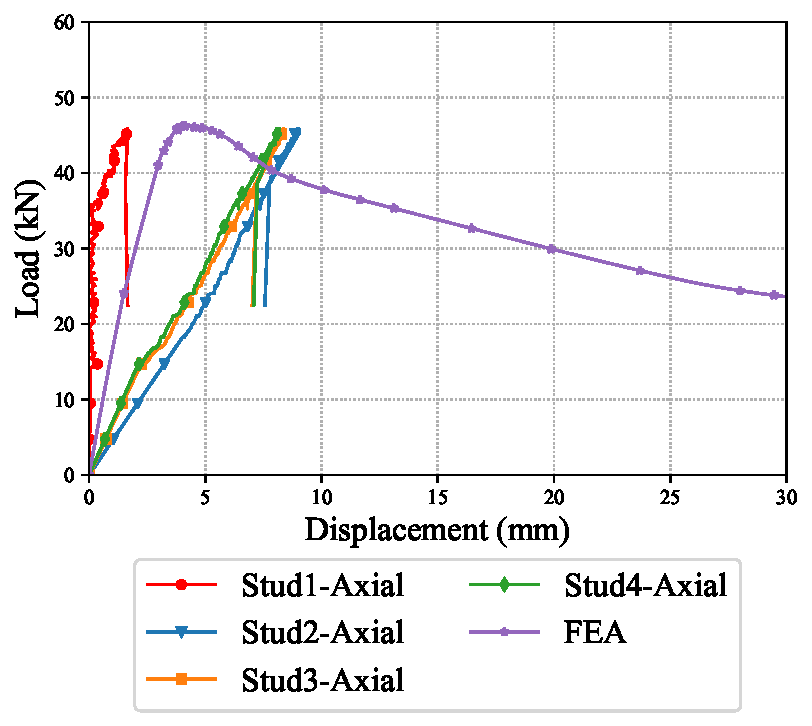
\includegraphics[scale=0.65]{AT3-Load-Axial-Exp-vs-FE.pdf}\\
		\caption{Test-AT3 FEA and experimental results comparison - Applied load versus axial displacement}
		\label{fig:AT3-fea}
\end{figure}
\begin{figure}[!htbp]
	\centering
	\begin{subfigure}[b]{0.45\textwidth}
		\centering
		\includegraphics[width=\textwidth]{AT3-buckling-FEA.pdf}
		\caption{}
		\label{subfig:AT3-buckling-FEA}
	\end{subfigure}
	\begin{subfigure}[b]{0.45\textwidth}
		\centering
		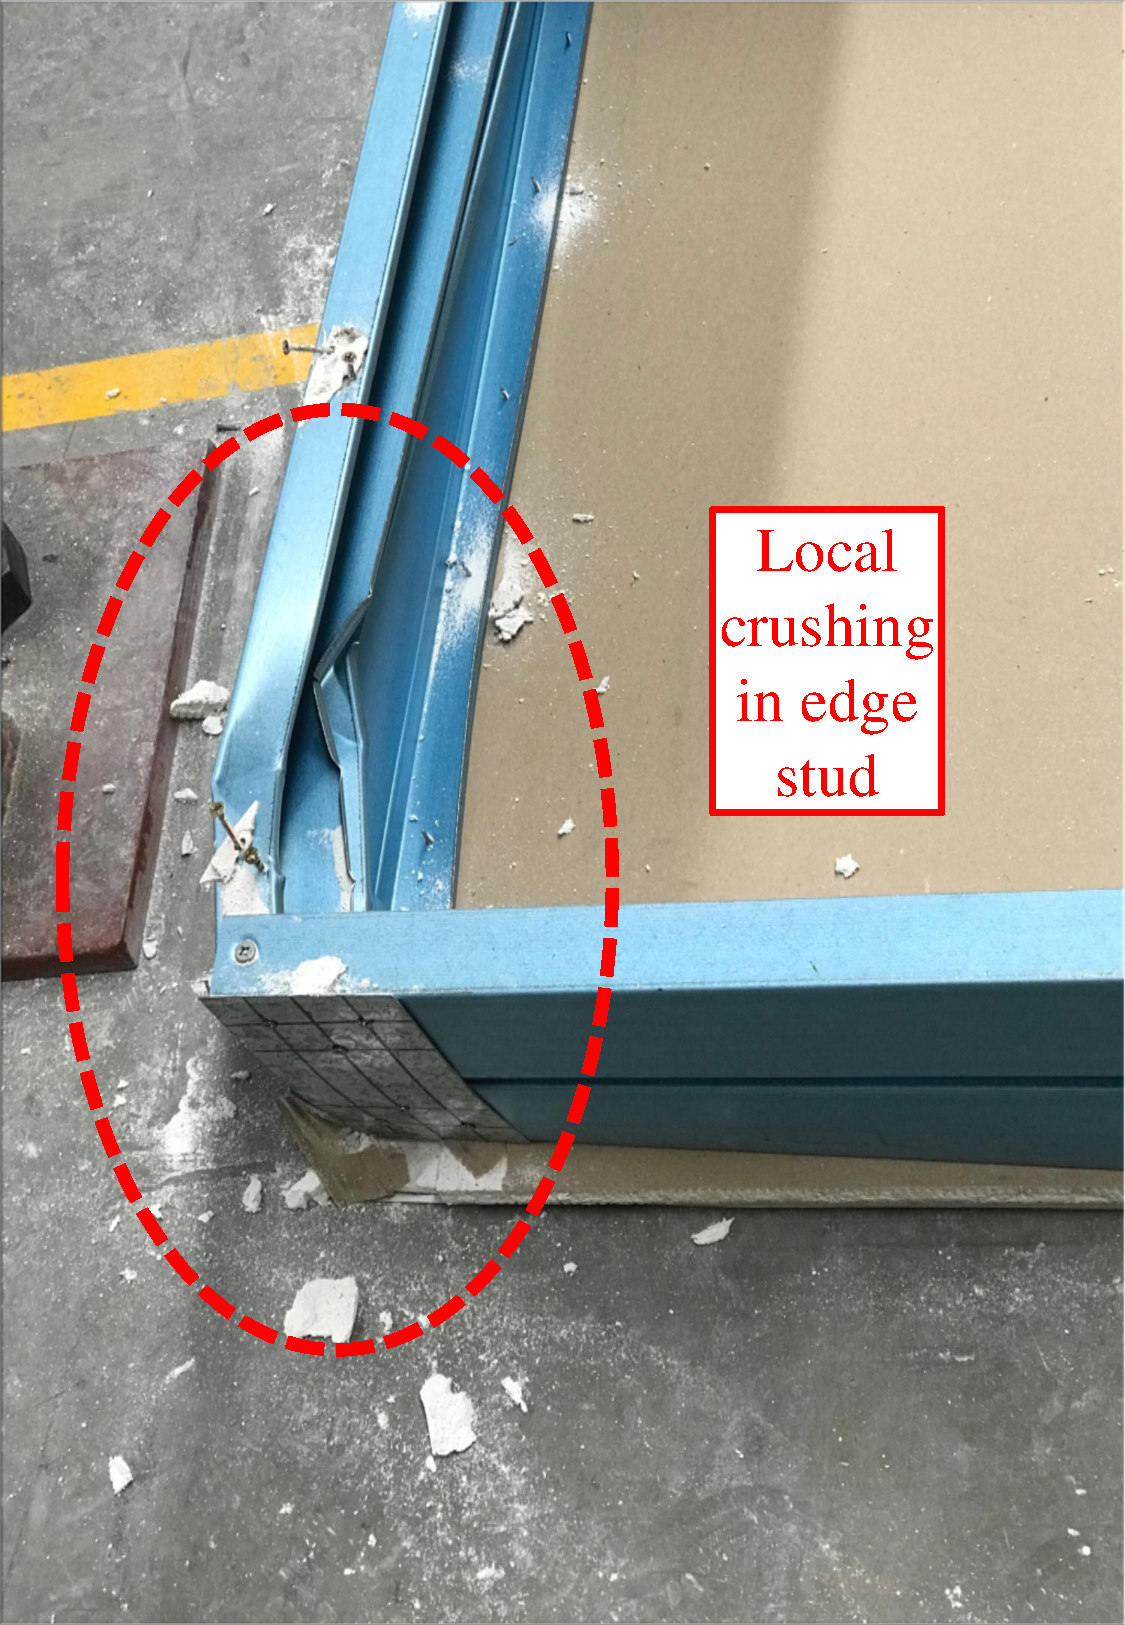
\includegraphics[width=\textwidth]{AT3-stud-crushing.pdf}
		\caption{}
		\label{subfig:AT3-buckling-experiment}
	\end{subfigure}
	   \caption{Test-AT3 - Buckling of studs (a) FEA (b) Experiment}
	   \label{fig:AT3-buckling-fea-comparison}
\end{figure} 

\subsection*{Test-AT4}

Test-AT4 was conducted on double stud LSF walls with 70 mm deep 0.95 mm thick studs as shown in \Cref{fig:AT4-plan-fea}. FE structural model resulted an axial compression capacity of 71.81 kN as shown in \Cref{fig:AT4-fea}. However the experimental Test-AT4 resulted an axial compression capacity of 86.21 kN. The structural FE model prediction was 14.4 kN less than the experimental results. This increased ambient temperature stud capacity might be attributed by the higher yield strength of the studs used in the test wall. As the steel studs for Test-AT4 were procured as a different lot resulting in different batch of steel used for cold-forming the studs, the test wall resulted in a higher axial compression capacity. However, the yield strength values used in the structural FE model was constant for all the tests. Another reason for increased axial compression capacity from the experiment may be due to the load sharing to the strengthened edge studs. However, the influence of the strengthened edge studs was not considered in this research and needs further investigation. The buckling of web and flanges observed in the studs during experimental investigation could be predicted by the developed structural FE model as shown in \Cref{fig:AT4-buckling-fea-comparison}.
\begin{figure}[!htbp]
	\centering
			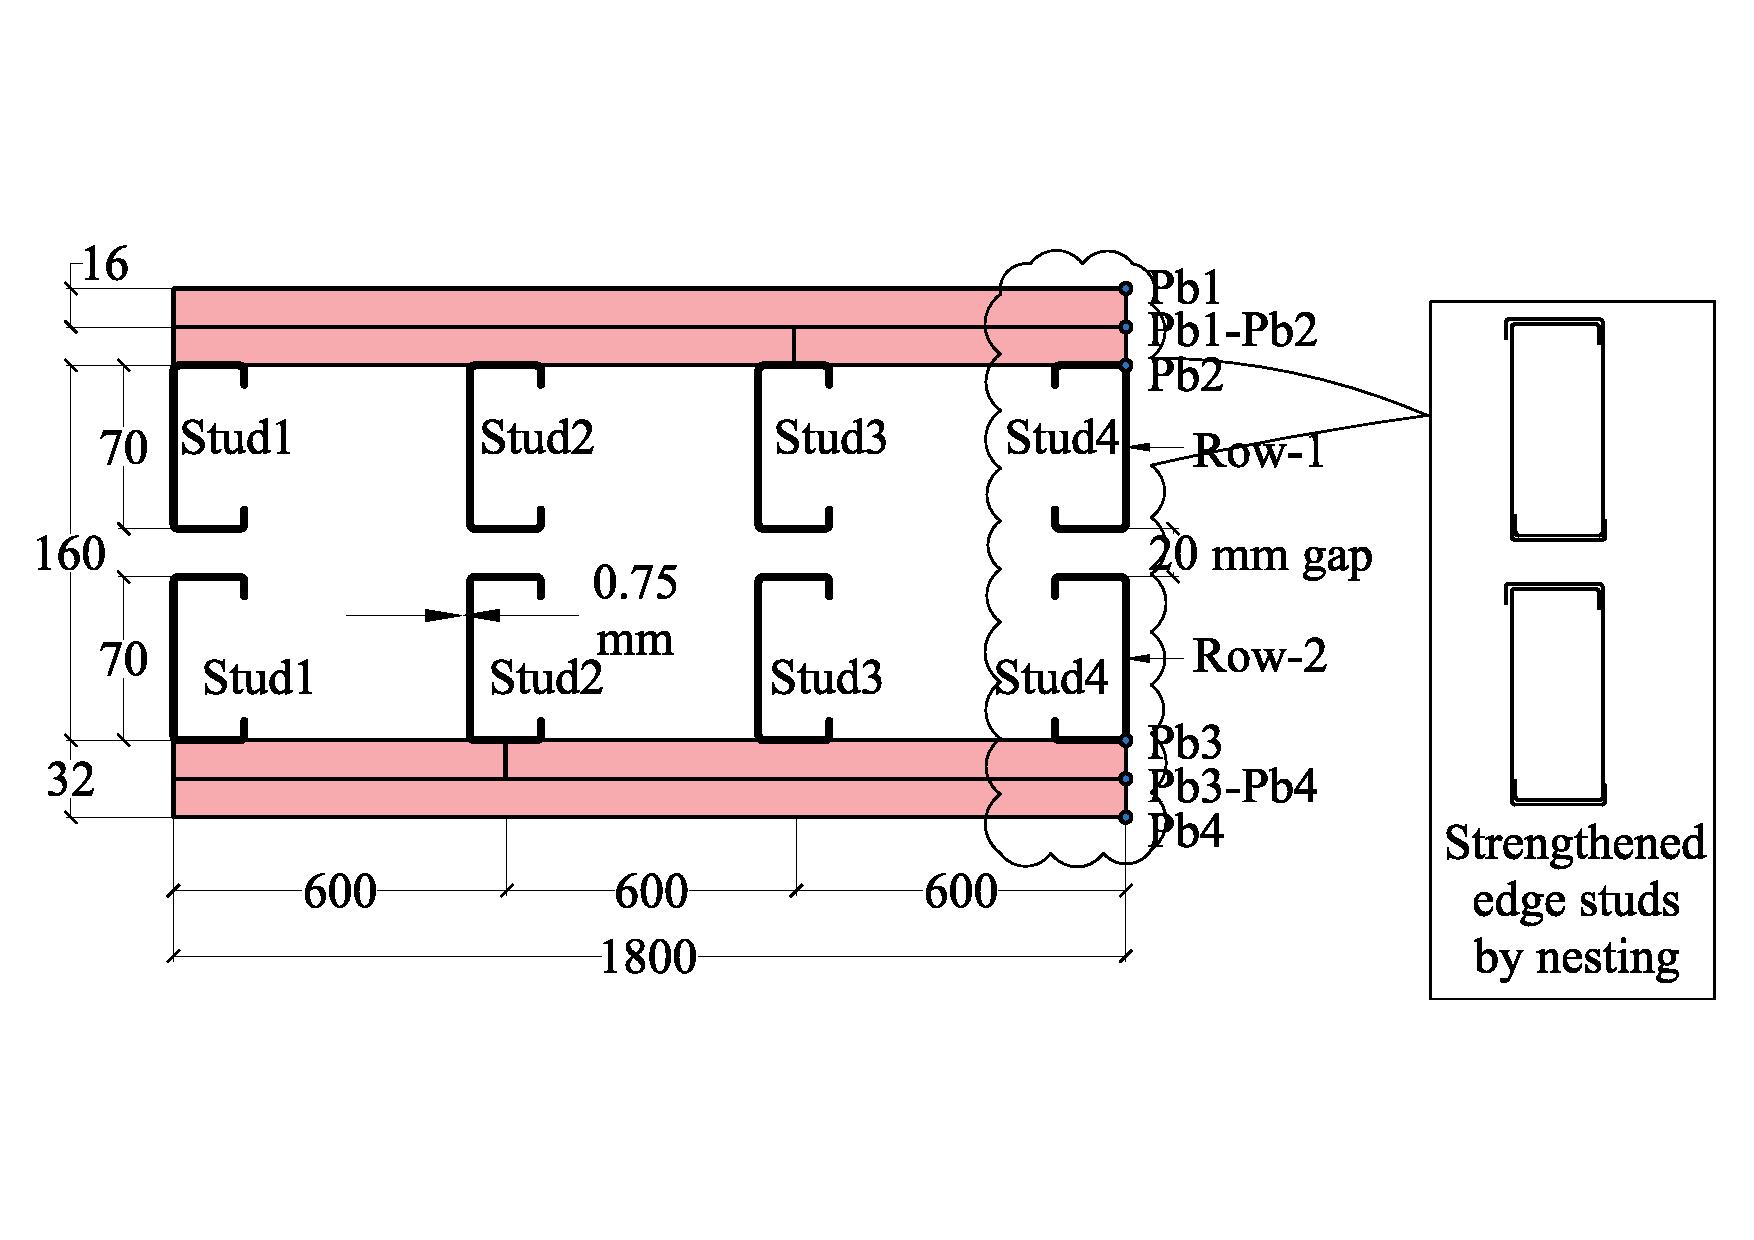
\includegraphics[scale=0.25]{AT4-plan.pdf}\\
		\caption{Test-AT4 plan}
		\label{fig:AT4-plan-fea}
\end{figure}
\begin{figure}[!htbp]
	\centering
			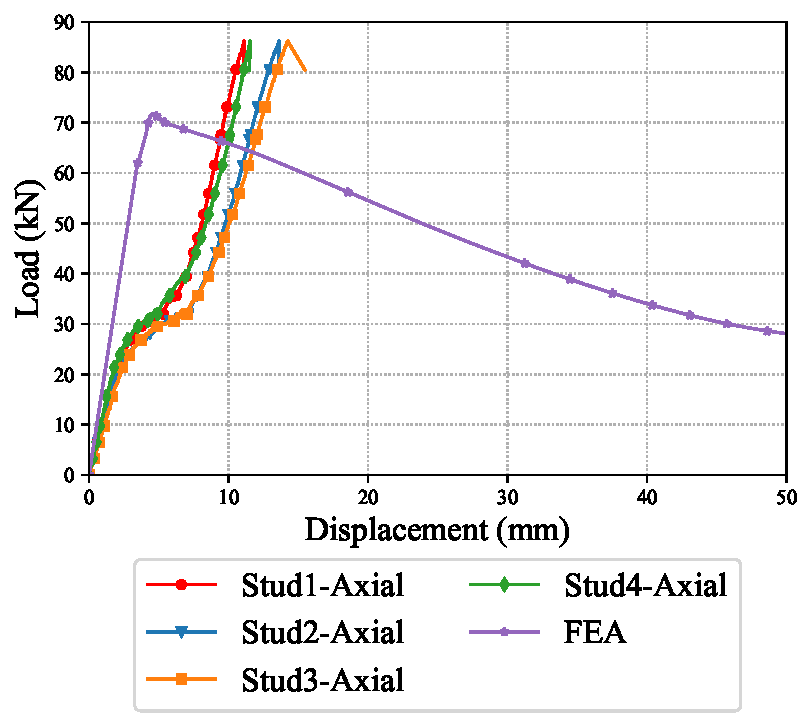
\includegraphics[scale=0.6]{AT4-Load-Axial-Exp-vs-FE.pdf}\\
		\caption{Test-AT4 FEA and experimental results comparison - Applied load versus axial displacement}
		\label{fig:AT4-fea}
\end{figure}
\begin{figure}[!htbp]
	\centering
	\begin{subfigure}[b]{0.35\textwidth}
		\centering
		\includegraphics[width=\textwidth]{AT4-buckling-FEA.pdf}
		\caption{}
		\label{subfig:AT4-buckling-FEA}
	\end{subfigure}
	\begin{subfigure}[b]{0.35\textwidth}
		\centering
		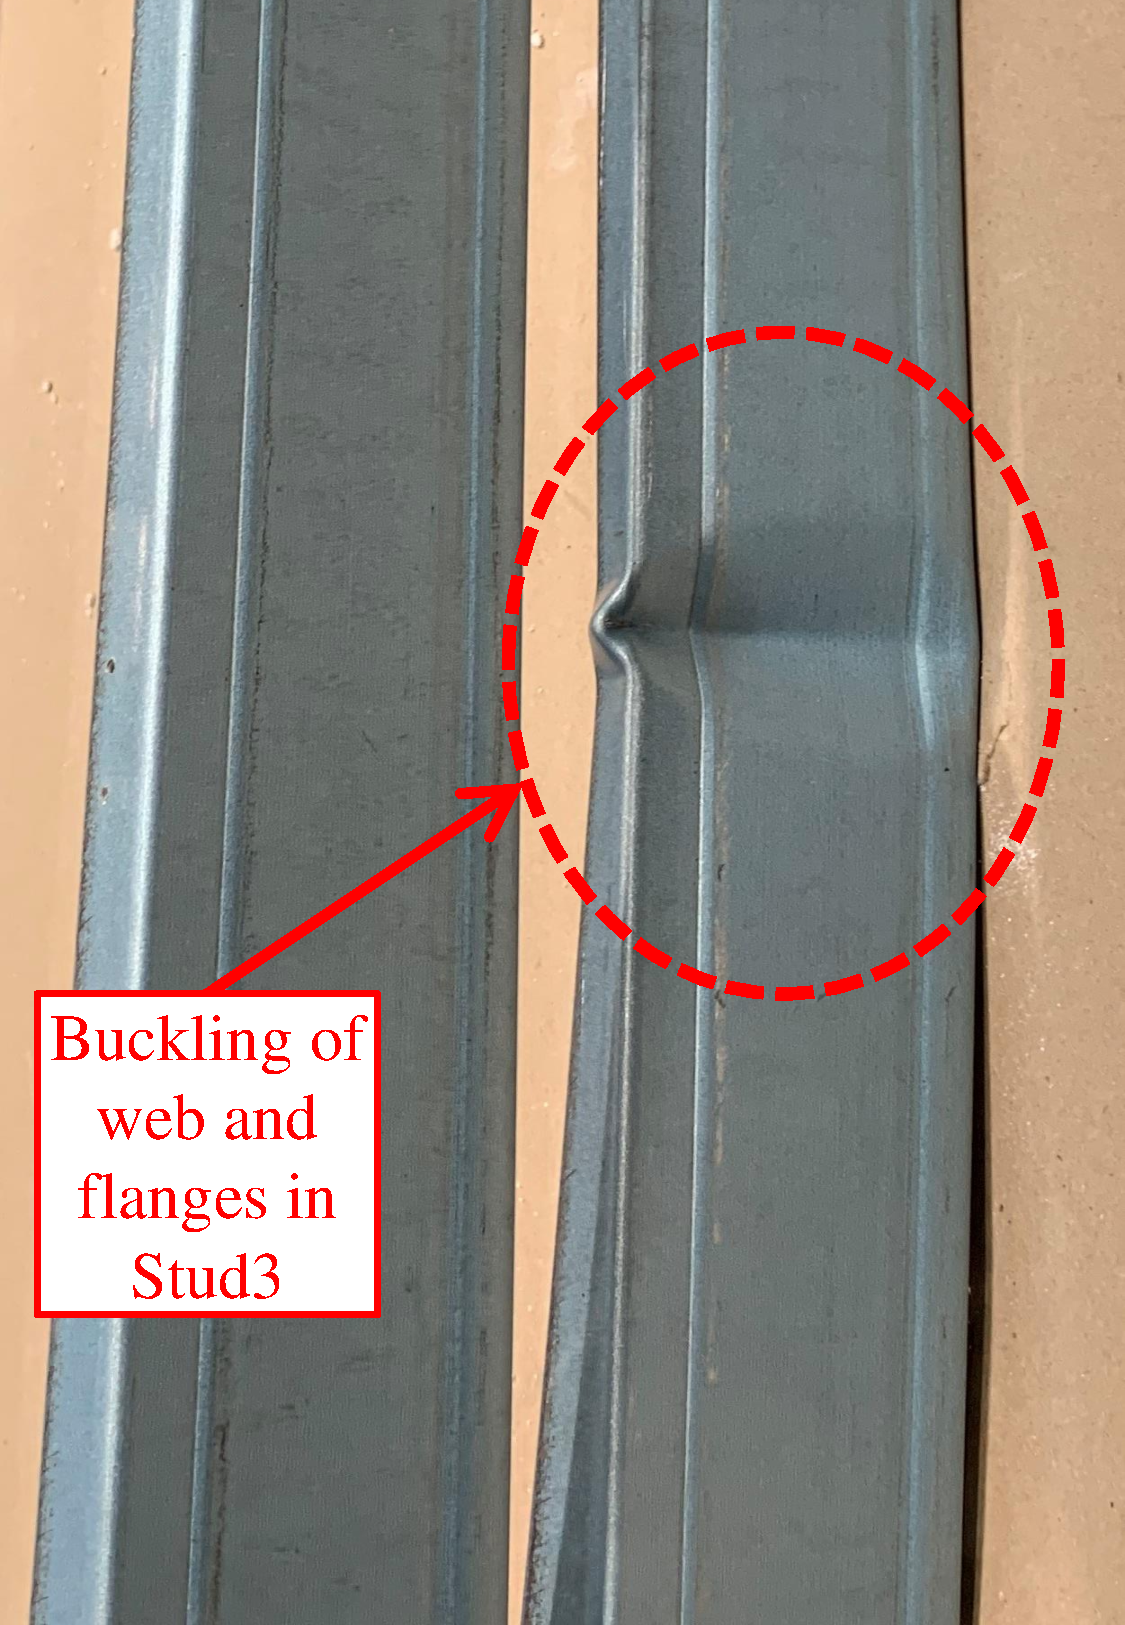
\includegraphics[width=\textwidth]{AT4-buckling.pdf}
		\caption{}
		\label{subfig:AT4-buckling-experiment}
	\end{subfigure}
	   \caption{Test-AT4 - Buckling of studs (a) FEA (b) Experiment}
	   \label{fig:AT4-buckling-fea-comparison}
\end{figure} 

\subsection*{Test-AT5}

Test-AT5 was conducted on staggered stud LSF wall as shown in \Cref{fig:AT5-plan-fea}. The modelling technique adapted to simulate the ambient capacity Test-AT5 was different in comparison with the other four ambient capacity tests. This because of the use of omega noggings in the experimental set-up. As the noggings were connected through the webs instead of flanges in the experimental test wall, similar set-up was adapted in the structural FE model. Firstly, service holes were made on the studs at 1 m interval. The studs were arranged at 300 mm apart in the ASSEMBLY. A Reference Point (RP) was created at the top and bottom CG of the system as shown in \Cref{subfig:AT5-mpc-constraint-top}. Top and bottom boundary conditions along with the axial load were applied through these RPs'. Partitions were created round the service holes to facilitate the application of MPC beam constraints. This was done by tie-constraints selecting the edges of the service holes as the slave edges connecting to a master node at the centre of service hole. A RP was created at the centre of all the service holes and the nogging restraints were provided as boundary condition. Translation along the x-axis was fixed at the RP to simulate minor axis restraints provided by the omega nogging on the stud web. Details about the MPC-constraints on the service holes of the studs are shown in \Cref{subfig:AT5-mpc-constraint-nogging}. Meshing near the stud service holes are critical in the structural FE model. Therefore, partitions were created around the stud service holes in the ASSEMBLY to create a sweep mesh around the service holes as shown in \Cref{subfig:AT5-mesh}. The structural analysis was conducted in a similar procedure to that of Tests-AT1 to AT4 incorporating the above-mentioned changes in the model.
\begin{figure}[!htbp]
	\centering
			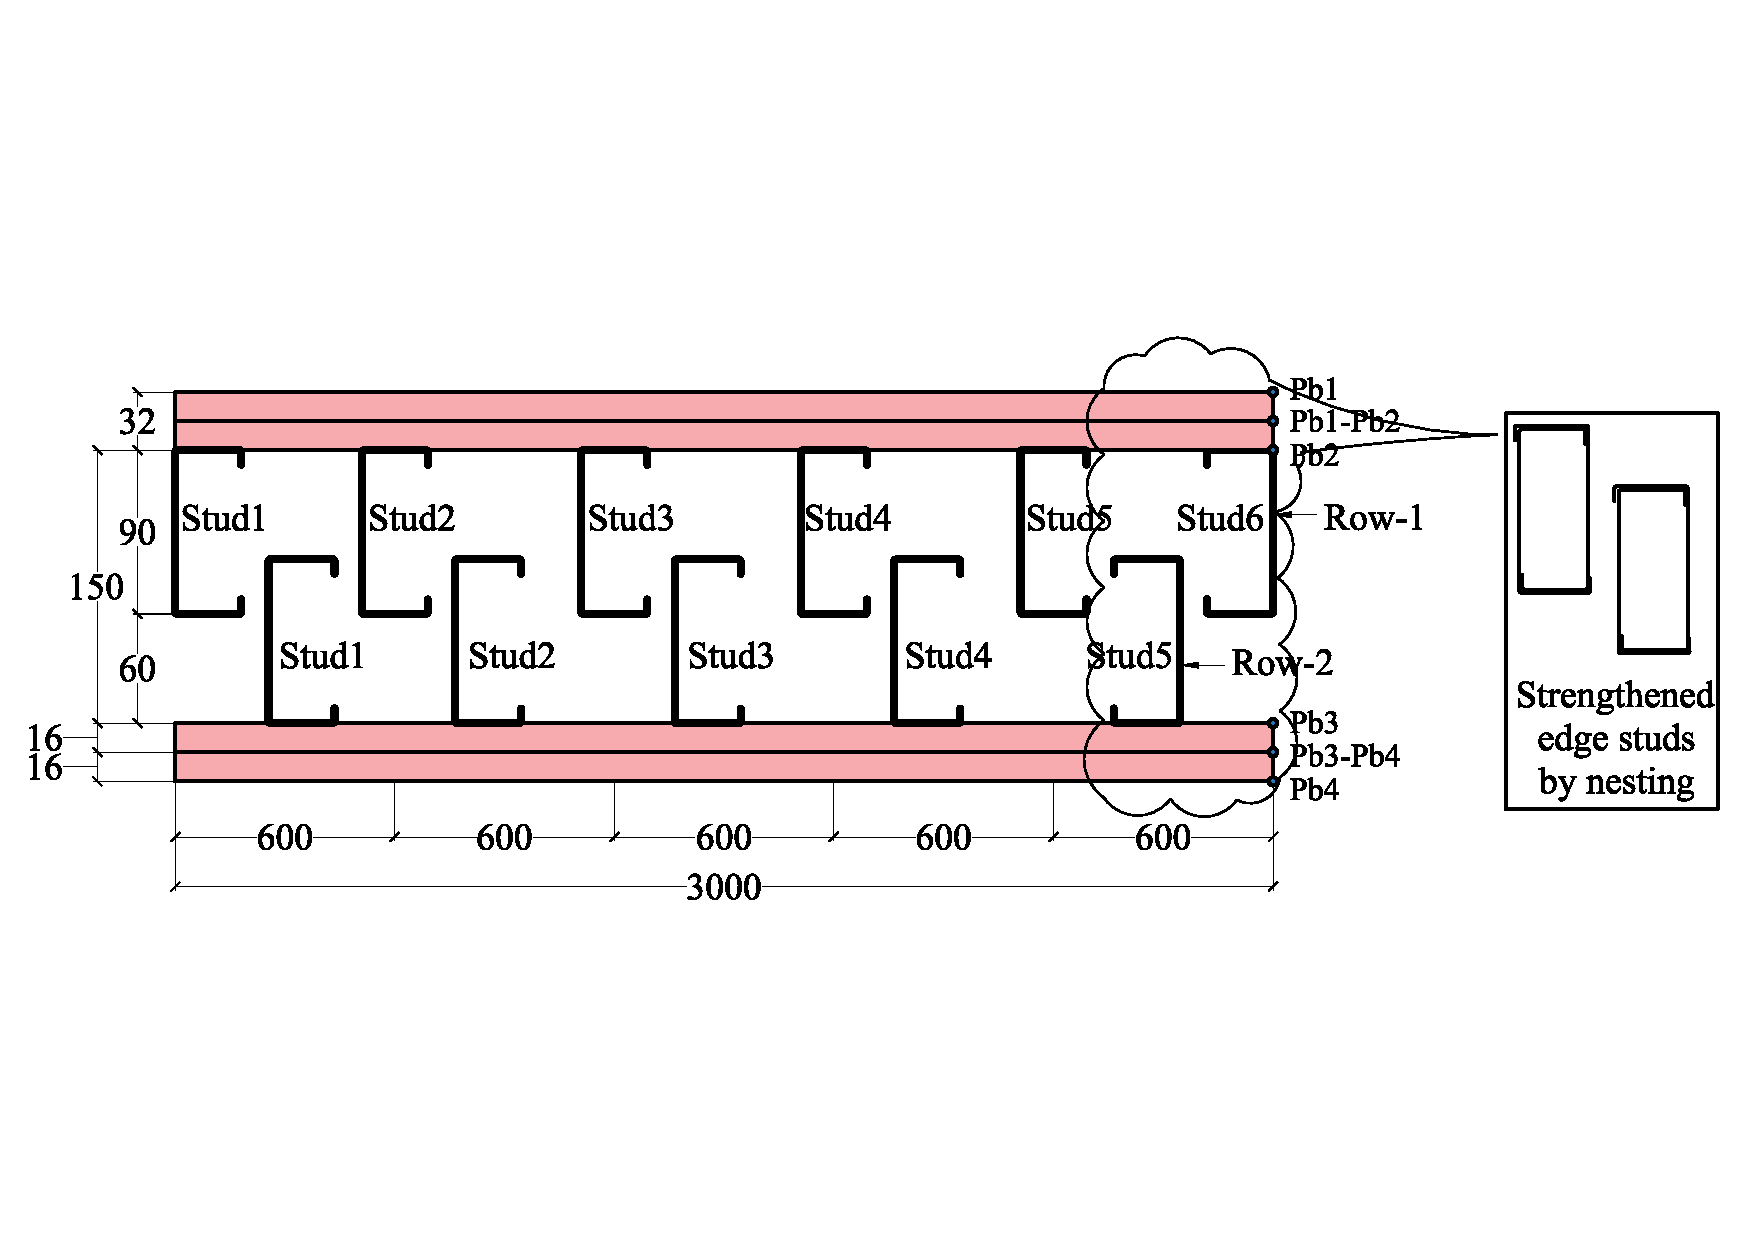
\includegraphics[scale=0.35]{AT5-plan.pdf}\\
		\caption{Test-AT5 plan}
		\label{fig:AT5-plan-fea}
\end{figure}    
\begin{figure}[!htbp]
	\centering
	\begin{subfigure}[b]{0.3\textwidth}
		\centering
		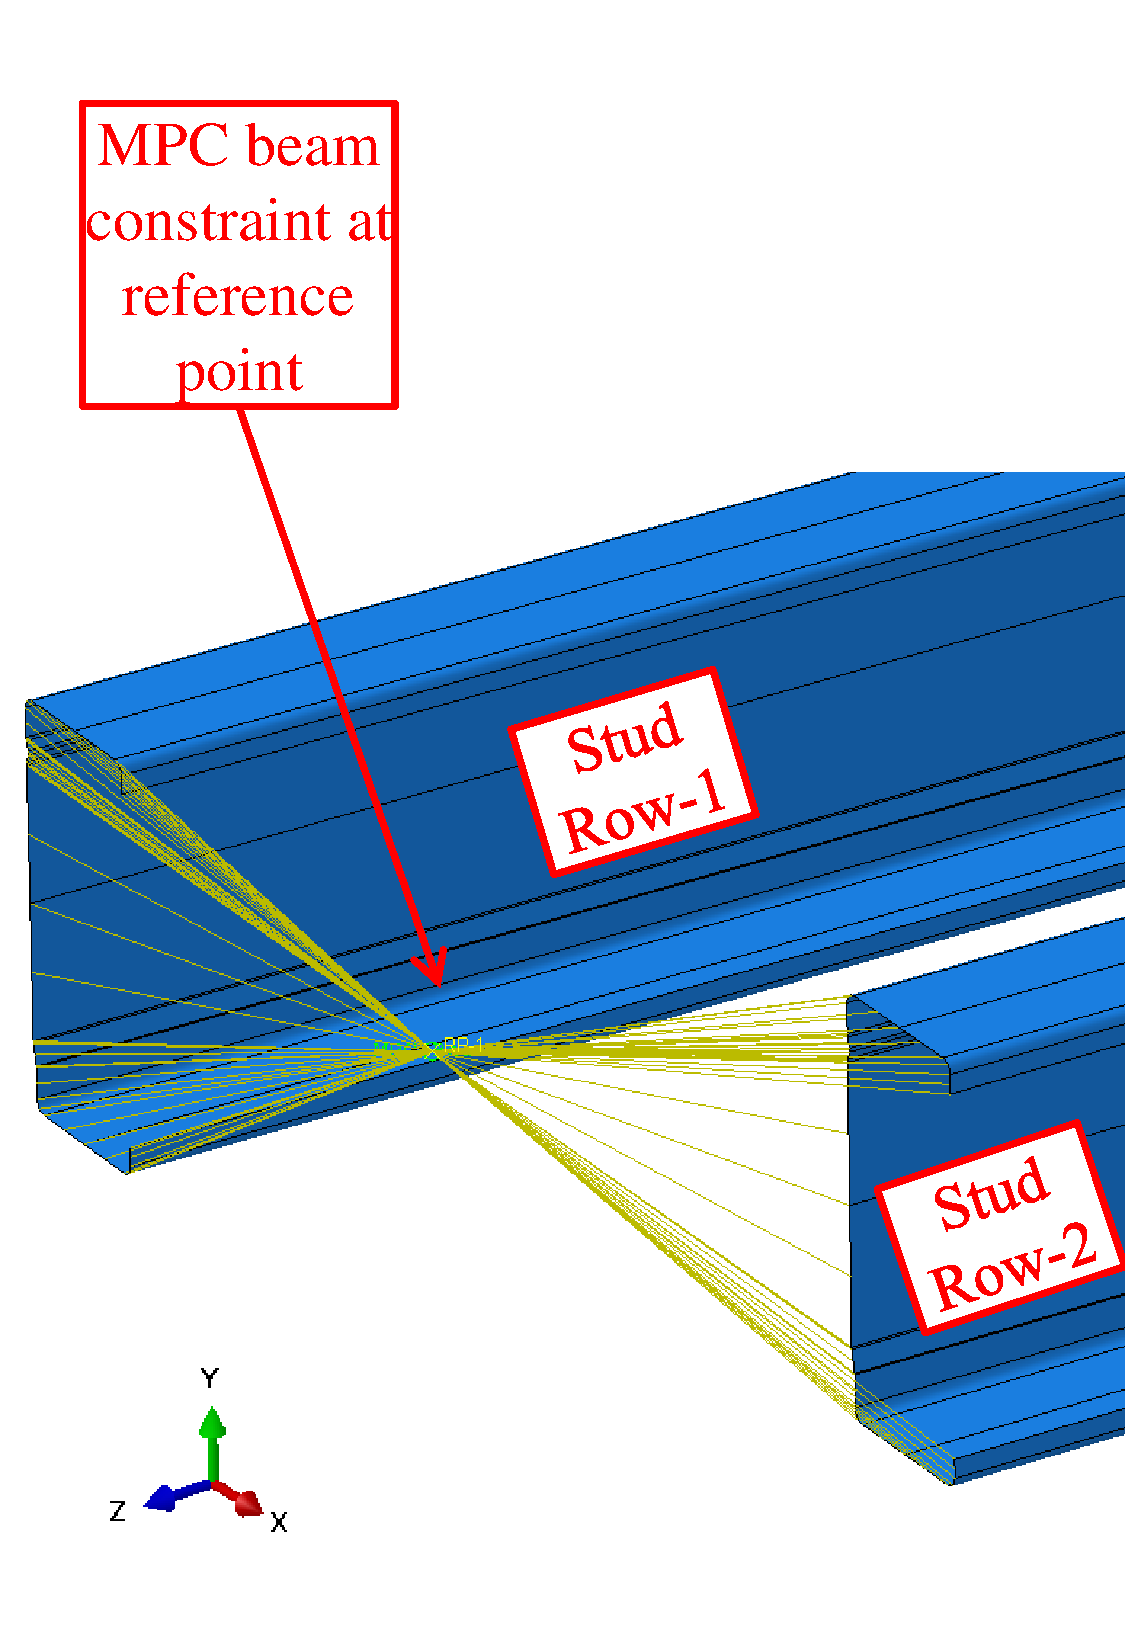
\includegraphics[width=\textwidth]{AT5-mpc-constraint-top.pdf}
		\caption{}
		\label{subfig:AT5-mpc-constraint-top}
	\end{subfigure}
	\begin{subfigure}[b]{0.5\textwidth}
		\centering
		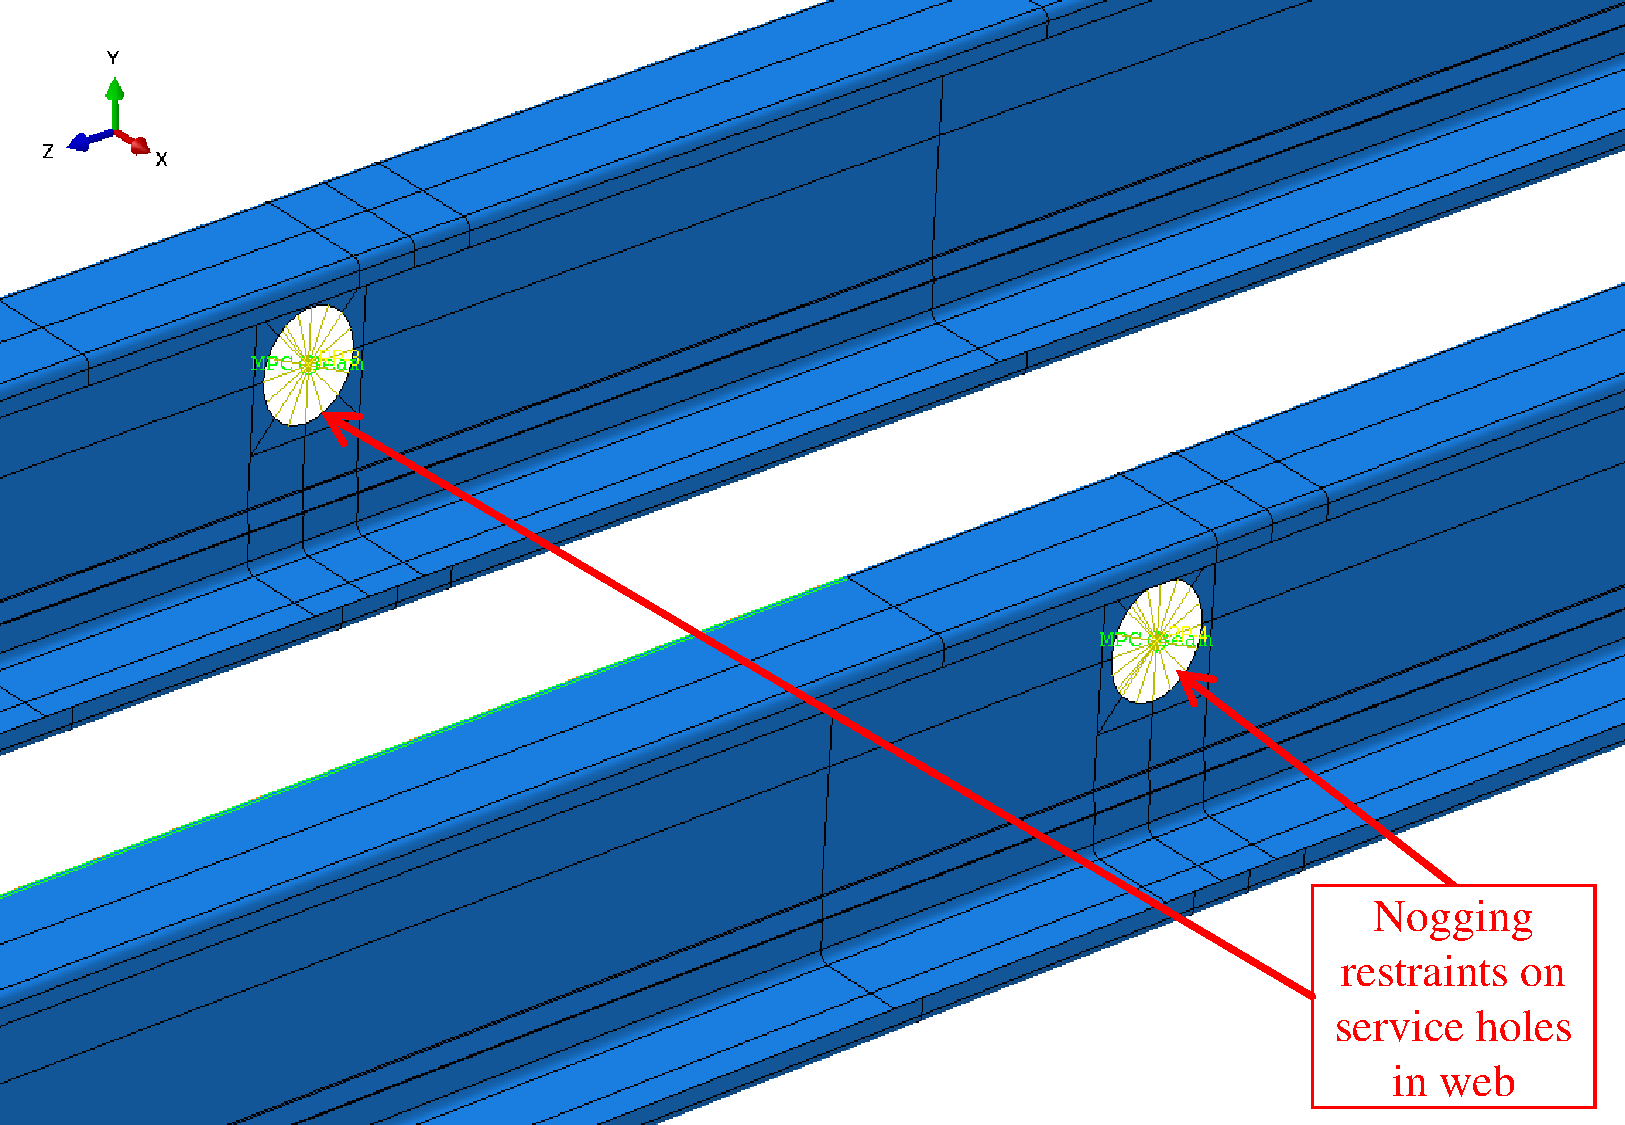
\includegraphics[width=\textwidth]{AT5-mpc-constraint-nogging.pdf}
		\caption{}
		\label{subfig:AT5-mpc-constraint-nogging}
	\end{subfigure}
	\begin{subfigure}[b]{0.5\textwidth}
		\centering
		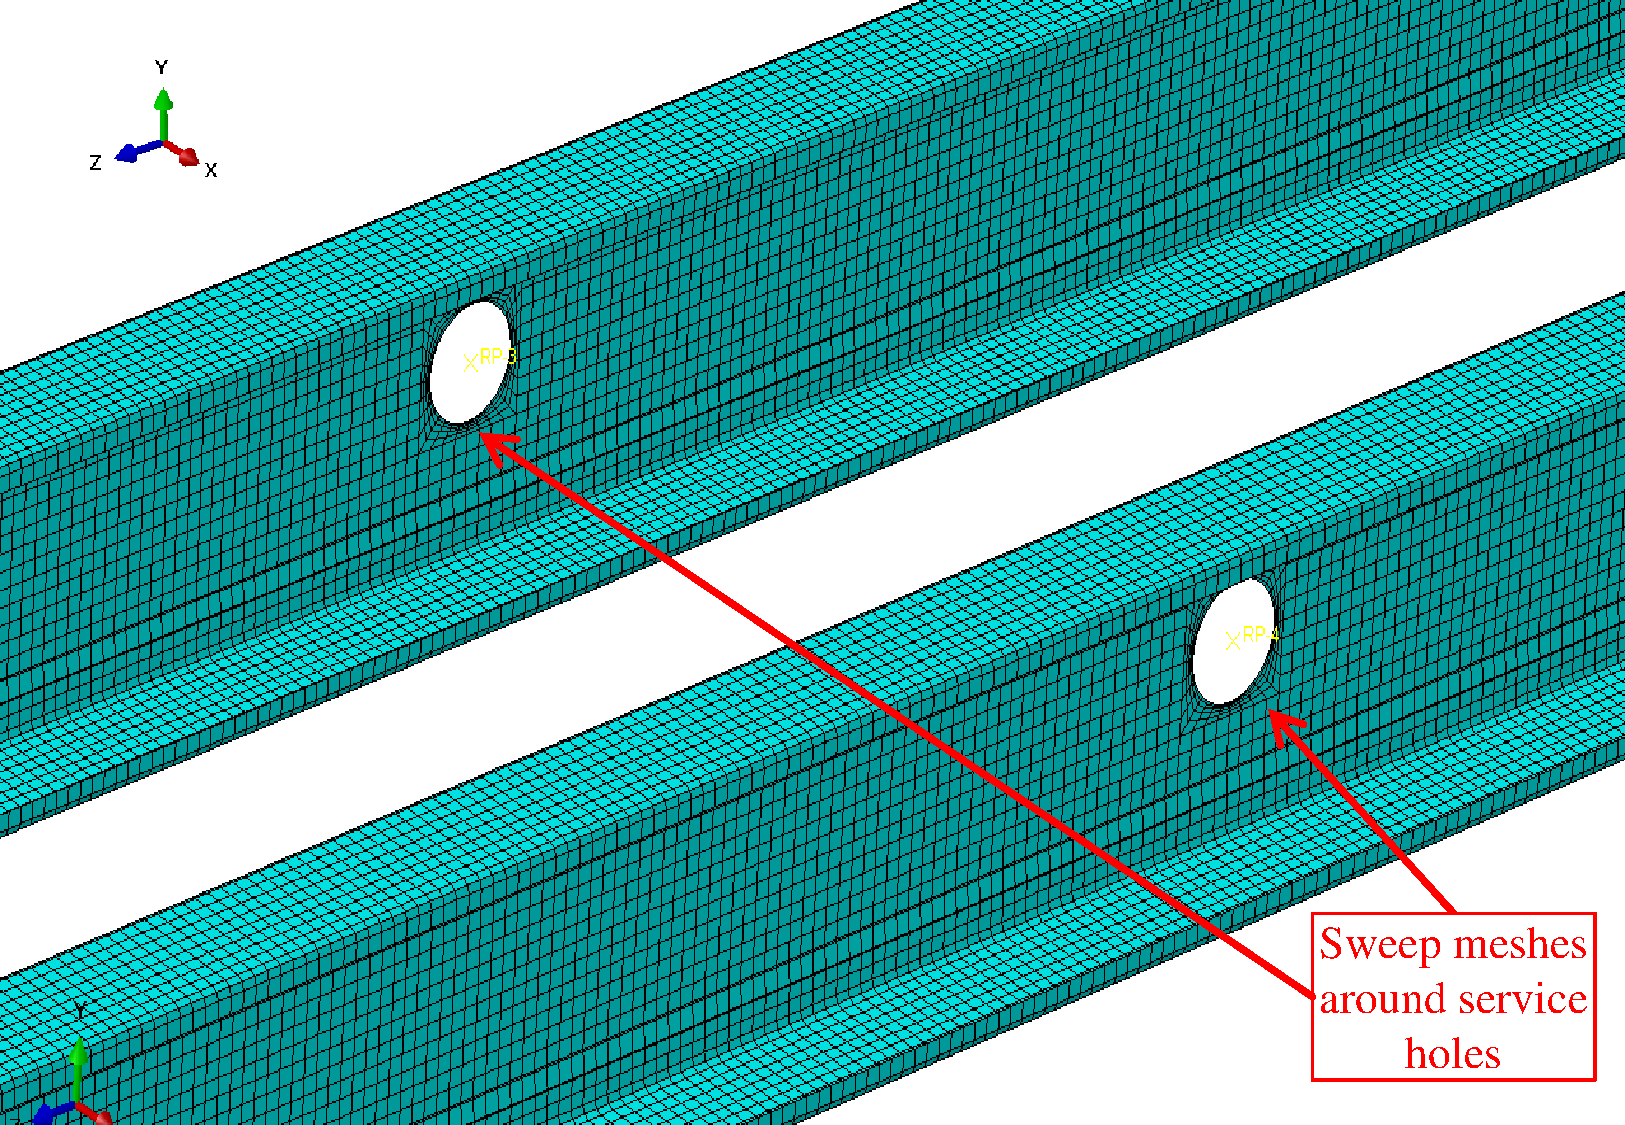
\includegraphics[width=\textwidth]{AT5-mesh.pdf}
		\caption{}
		\label{subfig:AT5-mesh}
	\end{subfigure}
	   \caption{Test-AT5 - Buckling of studs (a) FEA (b) Experiment}
	   \label{fig:AT5-modelling-fea}
\end{figure} 
\begin{figure}[!htbp]
	\centering
			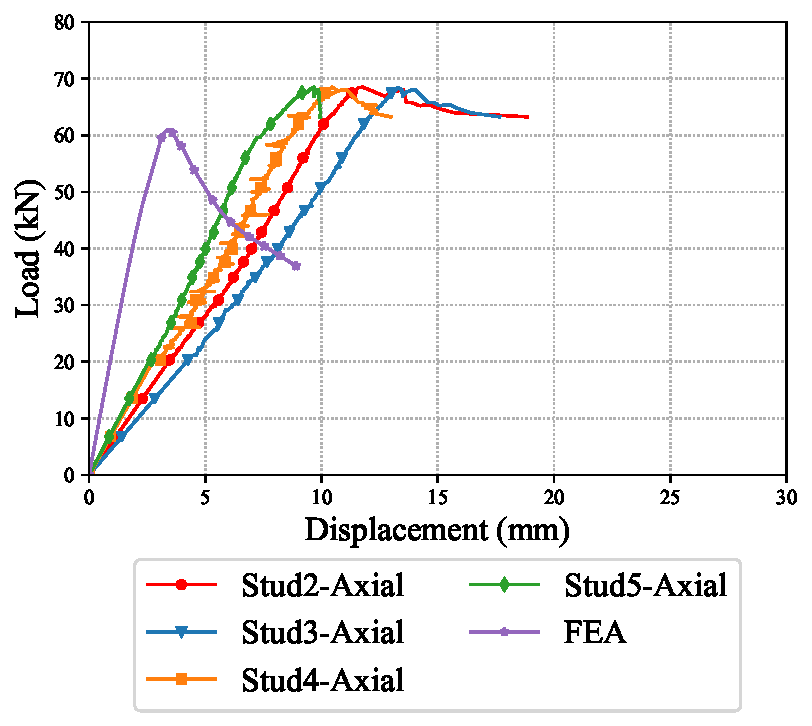
\includegraphics[scale=0.6]{AT5-Load-Axial-Exp-vs-FE.pdf}\\
		\caption{Test-AT5 FEA and experimental results comparison - Applied load versus axial displacement}
		\label{fig:AT5-fea}
\end{figure}
\begin{figure}[!htbp]
	\centering
	\begin{subfigure}[b]{0.4\textwidth}
		\centering
		\includegraphics[width=\textwidth]{AT5-buckling-FEA.pdf}
		\caption{}
		\label{subfig:AT5-buckling-FEA}
	\end{subfigure}
	\begin{subfigure}[b]{0.4\textwidth}
		\centering
		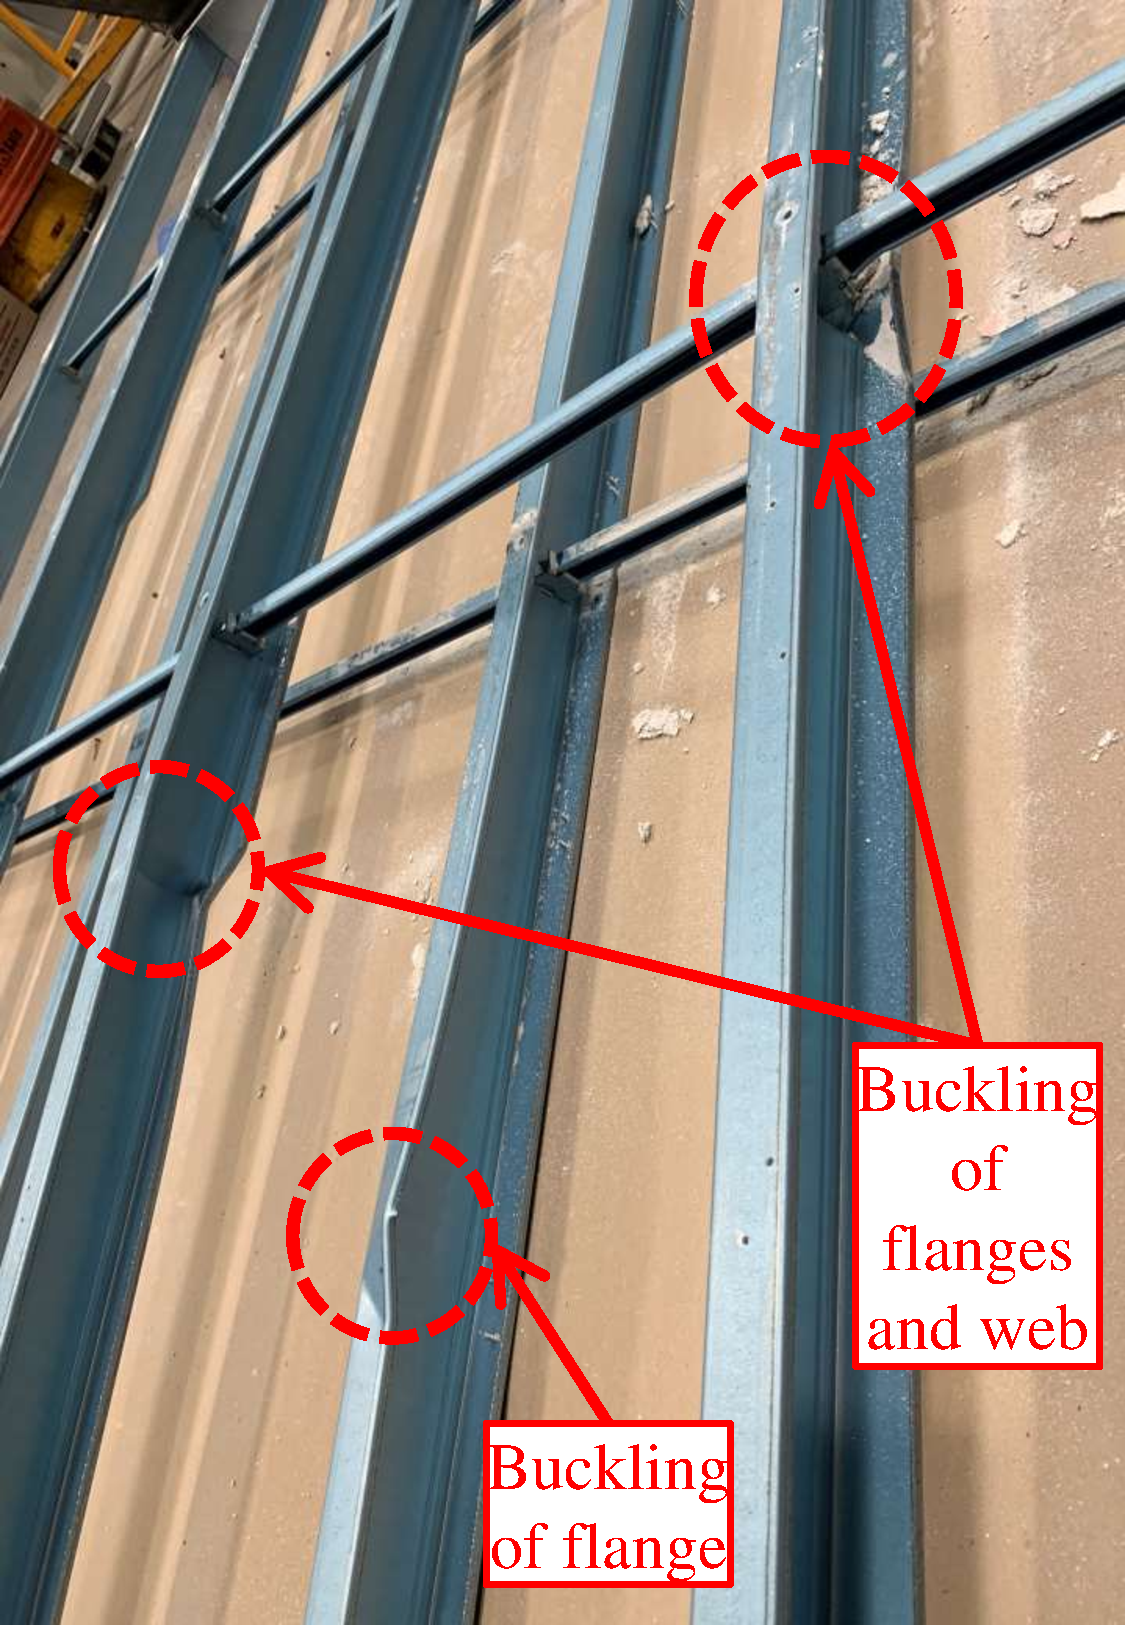
\includegraphics[width=\textwidth]{AT5-buckling.pdf}
		\caption{}
		\label{subfig:AT5-buckling-experiment}
	\end{subfigure}
	   \caption{Test-AT5 - Buckling of studs (a) FEA (b) Experiment}
	   \label{fig:AT5-buckling-fea-comparison}
\end{figure} 

\Cref{fig:AT5-fea} shows the load versus axial displacement curves comparison from structural FE model and experimental results. The FE model resulted an axial compression capacity of 60.98 kN while the experiments resulted a capacity of 68.49 kN. The FE model prediction was 7.51 kN lesser than the experimental results. Buckling of the stud web and flanges near the service holes experienced in the experimental investigation could also be simulated by the developed structural FE model as shown in \Cref{fig:AT5-buckling-fea-comparison}. 

\section{Summary of Ambient Temperature Capacity Predictions}

\begin{table}[!htbp]
	\centering
	\caption{Ambient temperature capacity test FE predictions - Summary}
	\begin{tabular}{ccccc}
		\toprule
		\multicolumn{1}{m{2.25em}}{\centering{Test Name}} & 
		\multicolumn{1}{m{8em}}{\centering{Description}} & 
		\multicolumn{1}{m{2.6em}}{\centering{Failure Load (kN) Test}} &
		\multicolumn{1}{m{2.6em}}{\centering{Failure Load (kN) FE}} &
		\multicolumn{1}{m{4.5em}}{\centering{FE Difference (kN)}} \\
		\midrule
		AT1  & Double Stud - 90$\times$0.95 - 4 studs & 73.00 & 71.97 & -1.03 \\
		AT2  & Double Stud - 90$\times$0.75 - 4 studs & 47.08 & 46.25 & -0.83 \\
		AT3  & Double Stud - 90$\times$0.75 - 6 studs & 39.42 & 46.25 & +6.83 \\
		AT4  & Double Stud - 70$\times$0.95 - 4 studs & 86.21 & 71.81 & -14.40 \\
		AT5  & Staggered Stud - 90$\times$0.95 - 6 studs & 68.49 & 60.98 & -7.51 \\
		\bottomrule
	\end{tabular}%
	\label{tab:ambient-test-results-fea}%
\end{table}%

A summary of the structural FE model predictions is show in \Cref{tab:ambient-test-results-fea}. It is evident from the conducted numerical investigation that the developed structural FE model could determine the structural failure capacity of the double and staggered stud LSF walls under ambient temperature conditions to a reasonable accuracy but for Test-AT4. However, the difference in prediction between the structural FE model and experimental results in Test-AT4 is 16.70 \%. Therefore, this structural FE model was further extended to include temperature boundary conditions in studs to predict the failure time of these complex LSF walls and is discussed next. 

\section[Coupled Temperature Displacement Structural Analysis]{Coupled Temperature Displacement \\Structural Analysis}\label{sec:temp-disp-structural}

After determining the ambient temperature capacity of the tests from \Cref{ch:Ambient}, the failure time of the tested LSF walls under fire from \Cref{ch:Fire} are considered for investigation. Full-scale fire Tests-T1 to T7 and T10 conducted under load-bearing conditions were considered for the numerical investigation in this chapter. The non-load bearing fire Tests-T8 and T9 were investigated in \Cref{ch:FE-Parametric}. Aim of the coupled temperature displacement structural analysis was to determine the failure time of the tested wall configurations under specified temperature boundary conditions along with axial compression load. 3D shell elements were used for the analysis using S4RT element which supports temperature degree of freedom. Temperatures on the hot and cold flanges were extracted from the FDS thermal models from \Cref{ch:FE-Thermal} and was incorporated as boundary conditions on to the stud hot and cold flanges in the structural model. Temperature boundary conditions on the stud webs were increased linearly based on the hot and cold flanges and applied to the stud nodes along the length as shown in \Cref{fig:temperature-gradient-stud}. Linear temperature variation along the web is governed by the number of mesh nodes on the stud web. However, the fire and ambient side hot and cold flanges had no variations in the input temperature boundary condition. Concentrated force from the initial non-linear structural ambient temperature analysis was applied at the reference point on the top of the FE model. 
\begin{figure}[!htbp]
	\centering
			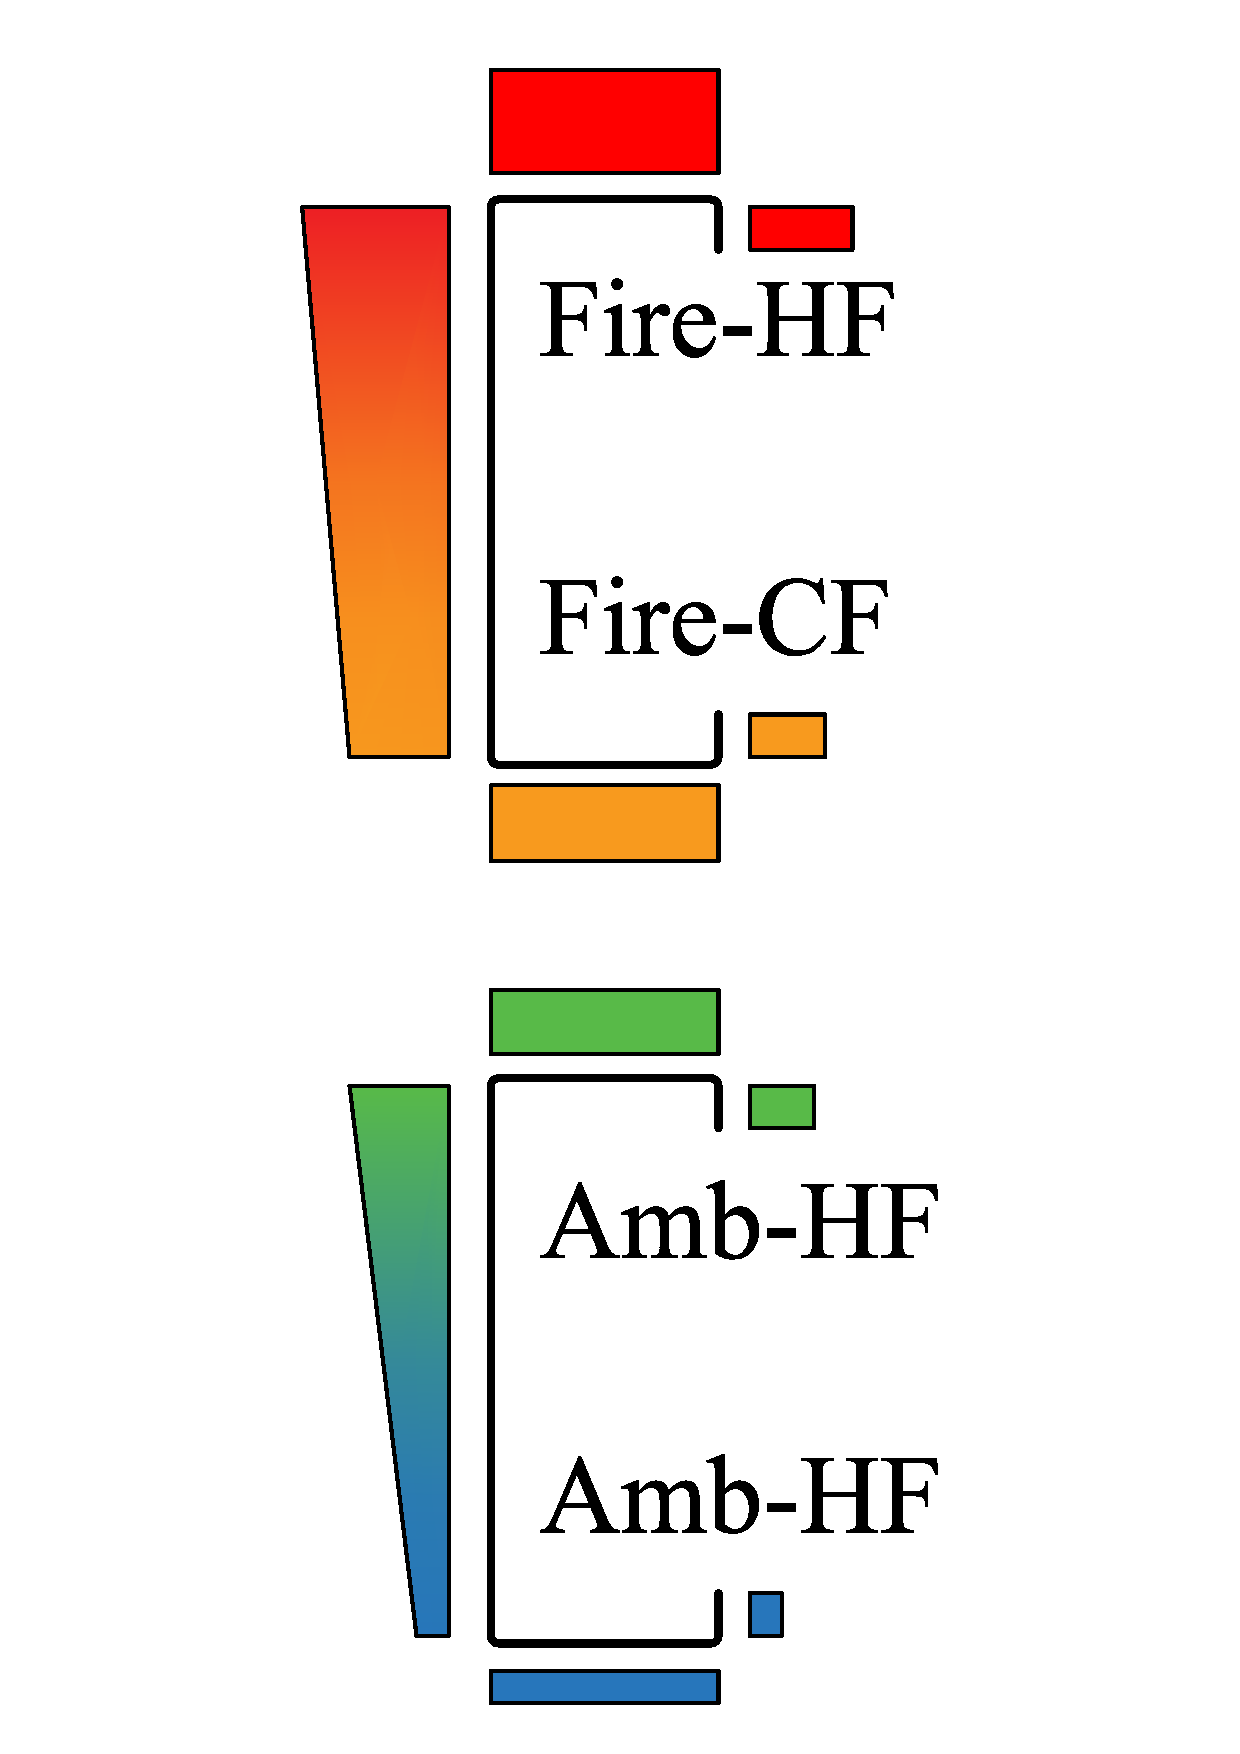
\includegraphics[scale=0.2]{temperature-gradient-stud.pdf}\\
		\caption{Temperature boundary condition gradient for typical double stud LSF wall}
		\label{fig:temperature-gradient-stud}
\end{figure}

Coupled-temperature displacement analysis was carried out to determine the structural response of studs under axial compression along with temperature boundary conditions. The applied axial load in the FE model was nearly equal to the LR used for the full-scale fire test in \Cref{ch:Fire}. Transient mode of analysis was adapted and the all the models were analysed for a time-period 240 min (14400 s). The effects of non-linearity was considered for the coupled temperature-displacement analysis. This method of structural analysis is generally referred to as sequentially coupled analysis wherein the thermal analysis is conducted firstly followed by the structural analysis. The output from thermal analysis acts as input to the structural analysis. The reactions were monitored on the bottom reference point and the axial displacement was monitored on the top reference point of the model at CG using history output feature in ABAQUS. The monitored data is stored in an output database file (ODB) and later used for post-processing. 
\begin{figure}[!htbp]
	\centering
	\begin{subfigure}[b]{0.45\textwidth}
		\centering
		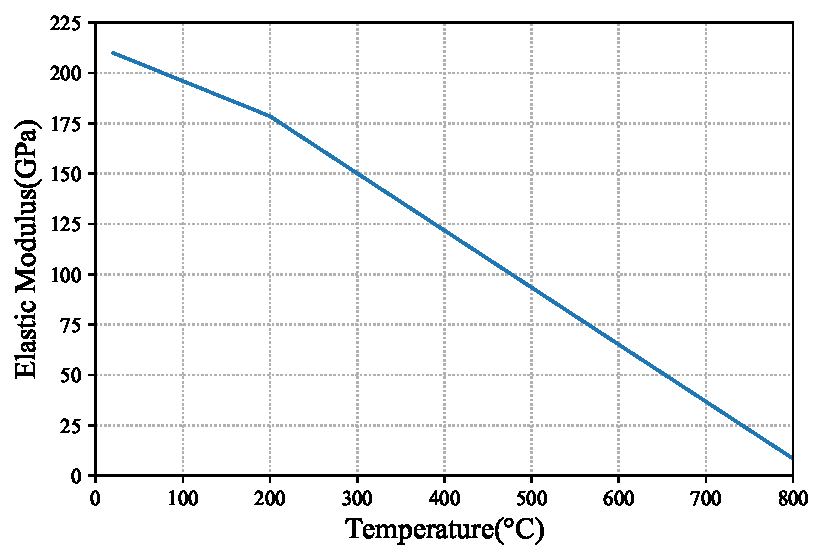
\includegraphics[width=\textwidth]{Steel-elastic-modulus.pdf}
		\caption{}
		\label{subfig:Steel-elastic-modulus}
	\end{subfigure}
	\begin{subfigure}[b]{0.45\textwidth}
		\centering
		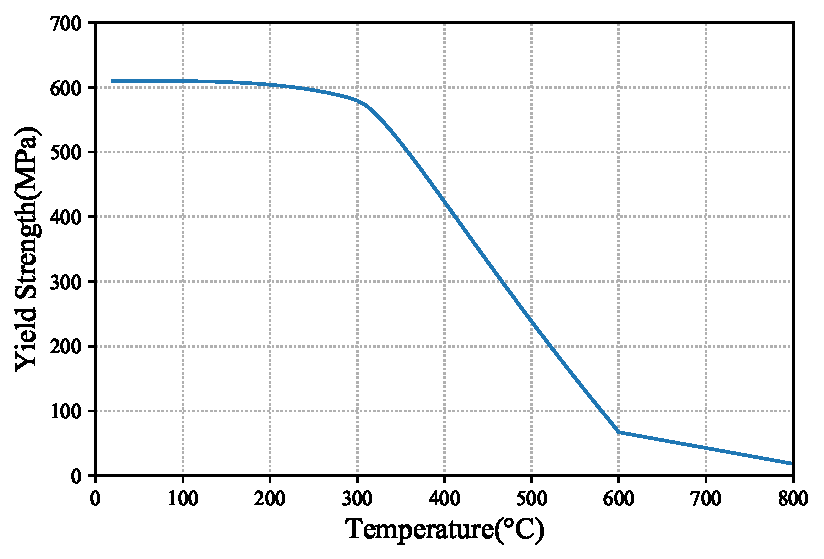
\includegraphics[width=\textwidth]{Steel-yield-strength.pdf}
		\caption{}
		\label{subfig:Steel-yield strength}
	\end{subfigure}
	   \caption{Elevated temperature mechanical properties of G550 steel from \citet{Kankanamge2011}}
	   \label{fig:steel-elevated-mechanical}
\end{figure} 

As the coupled temperature-displacement structural analysis include the effects of temperatures, the material properties used in the model had to account for the variations at elevated temperatures. Therefore, the elevated temperature mechanical properties for cold-formed steel were extracted from \citet{Kankanamge2011} which was verified by \citet{Rokilan2019}. The elevated temperature mechanical properties of steel such as elastic modulus and yield strength used in the FE model are shown in \Cref{fig:steel-elevated-mechanical}. As the coupled-temperature displacement analysis involves solving two boundary conditions such as temperature and axial compression load at the same time, there arises severe convergence issues with the FE model. This is because of the non-linear nature of the problem resulting in large deformations in the model. The non-linear nature of the model is largely due to the usage of thin-walled elements as studs. Treating these instabilities with a global solution might not best fit the problem. This was addressed by the introduction of automatic damping factor and adaptive stabilization factor during the analysis. This helps the models to converge to the desired solution. However, determining these factors are based on trial and error method and varies with the models as stated in the ABAQUS documentation manual (\cite{abaqus2017}). Therefore, the failure criteria of a model is determined either by comparing the reduction in the applied axial load with respect to time or with respect to axial displacement or with lateral deflection or a combination of the aforesaid. The selection of the failure criteria in the FE model depends on the convergence achieved in the given model based on the temperature boundary condition and applied axial loads. 

\section*{Test-T1}

Test-T1 was conducted on non-cavity insulated double stud LSF wall with 90 $\times$ 0.95 mm studs as shown in \Cref{fig:T1-plan-FEA}. Ambient temperature capacity FE model resulted an ultimate compression capacity of 71.9 kN. As the full-scale fire Test-T1 was conducted under 0.4 LR an axial compression capacity of 28.76 kN was applied to the model and coupled temperature displacement analysis was carried out. 
\begin{figure}[!htbp]
	\centering
			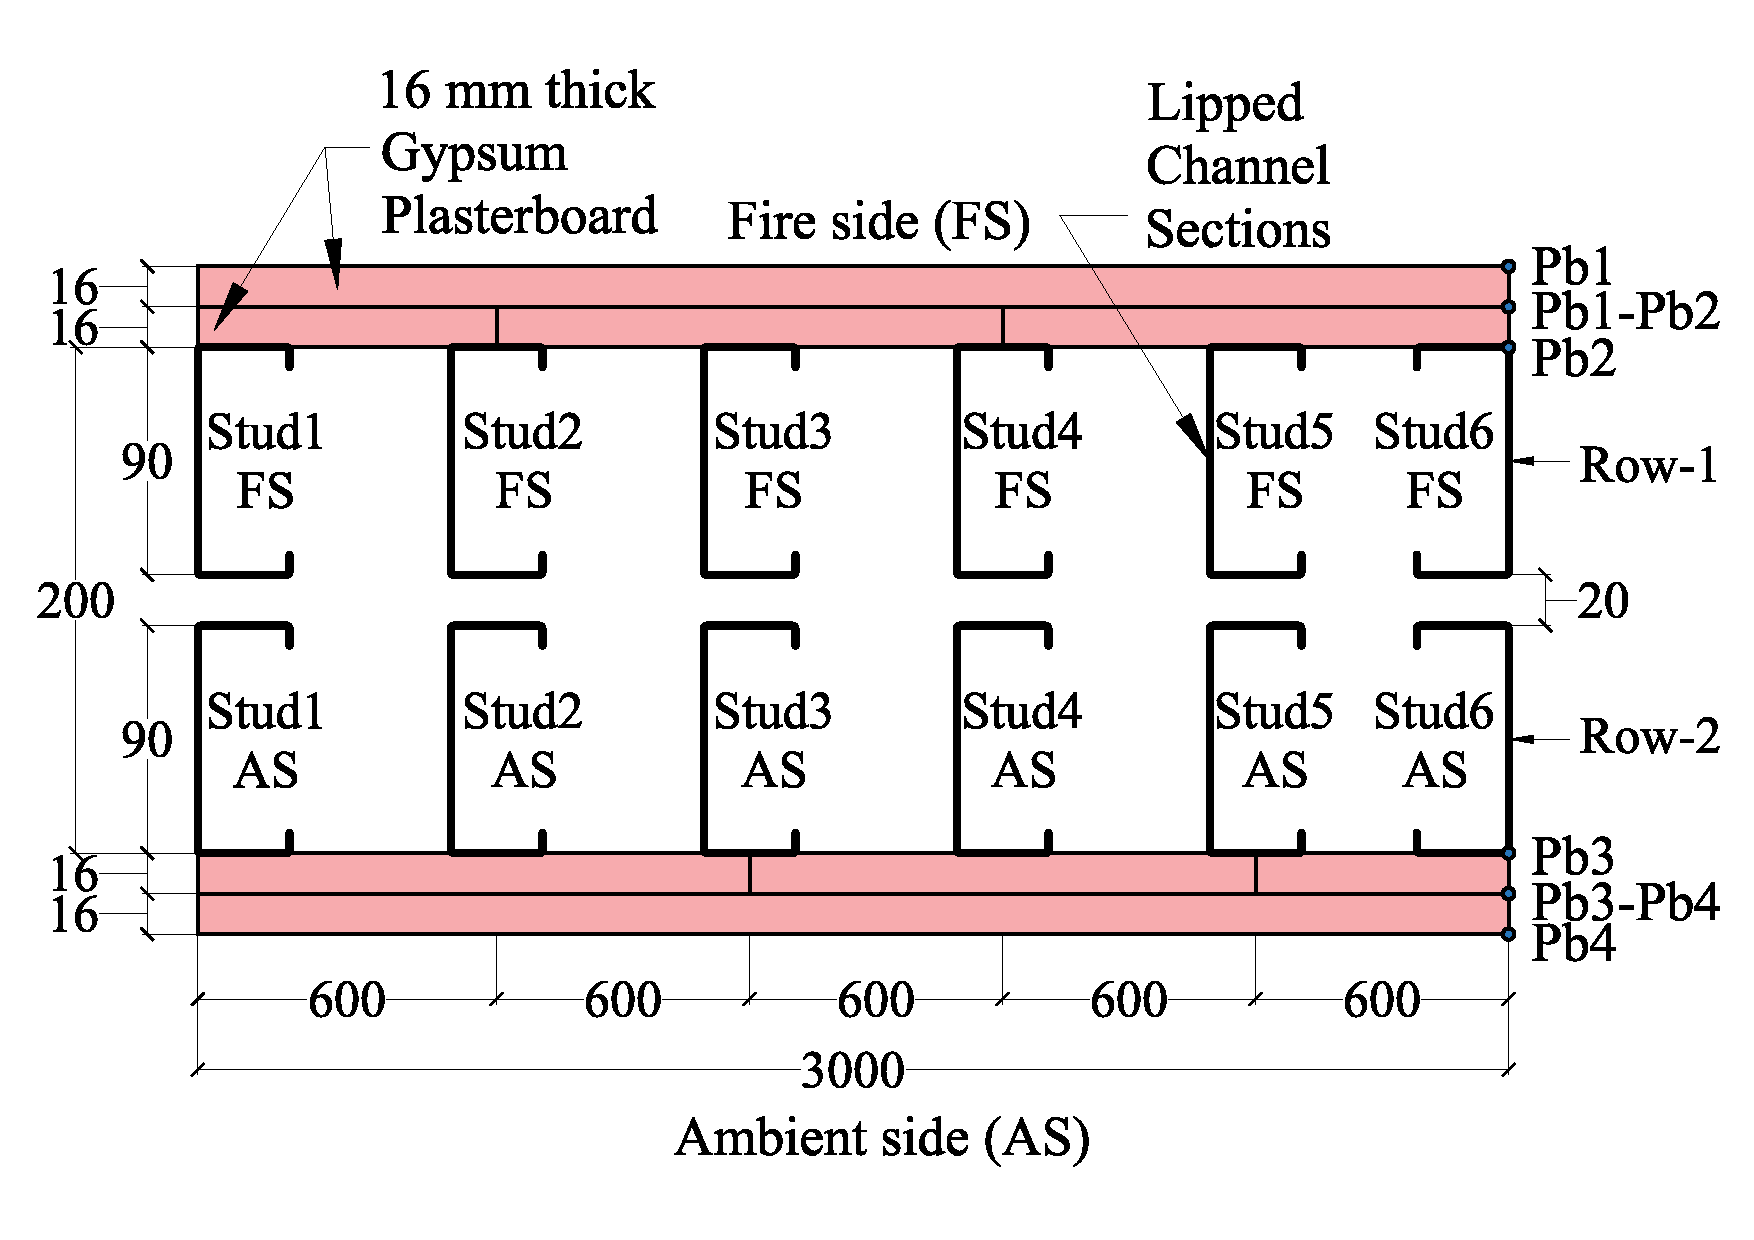
\includegraphics[scale=0.2]{T1-plan.pdf}\\
		\caption{Test-T1 plan view}
		\label{fig:T1-plan-FEA}
\end{figure}

The failure of the coupled temperature displacement model of Test-T1 was determined through the time versus axial displacement and lateral deflection curves extracted from the model as shown in \Cref{fig:T1-structural-FE-vs-Exp}. Buckling modes extracted from the FE model is shown in \Cref{subfig:T1-buckling-FEA}. Comparison with the buckling modes from experimental result in \Cref{subfig:T1-buckling-FEA-Exp} shows that the local buckling experienced in the full-scale fire test could not be predicted by the developed FE model. This was due to sever instability in the model causing convergence failure. However, the axial displacement and lateral deflection versus time curves could predict the failure time to reasonable agreement. The maximum axial displacement recorded in the fire Test-T1 was -8 mm while it was 12.75 mm from the FE model predictions. Likewise, the experiment resulted a lateral deflection of -14.44 mm while the FE model predictions resulted a lateral deflection of 18.6 mm. The failure time predicted by the structural FE model was 174 min while the experiment resulted a failure time of 176 min.  
\begin{figure}[!htbp]
	\centering
	\begin{subfigure}[b]{0.8\textwidth}
		\centering
		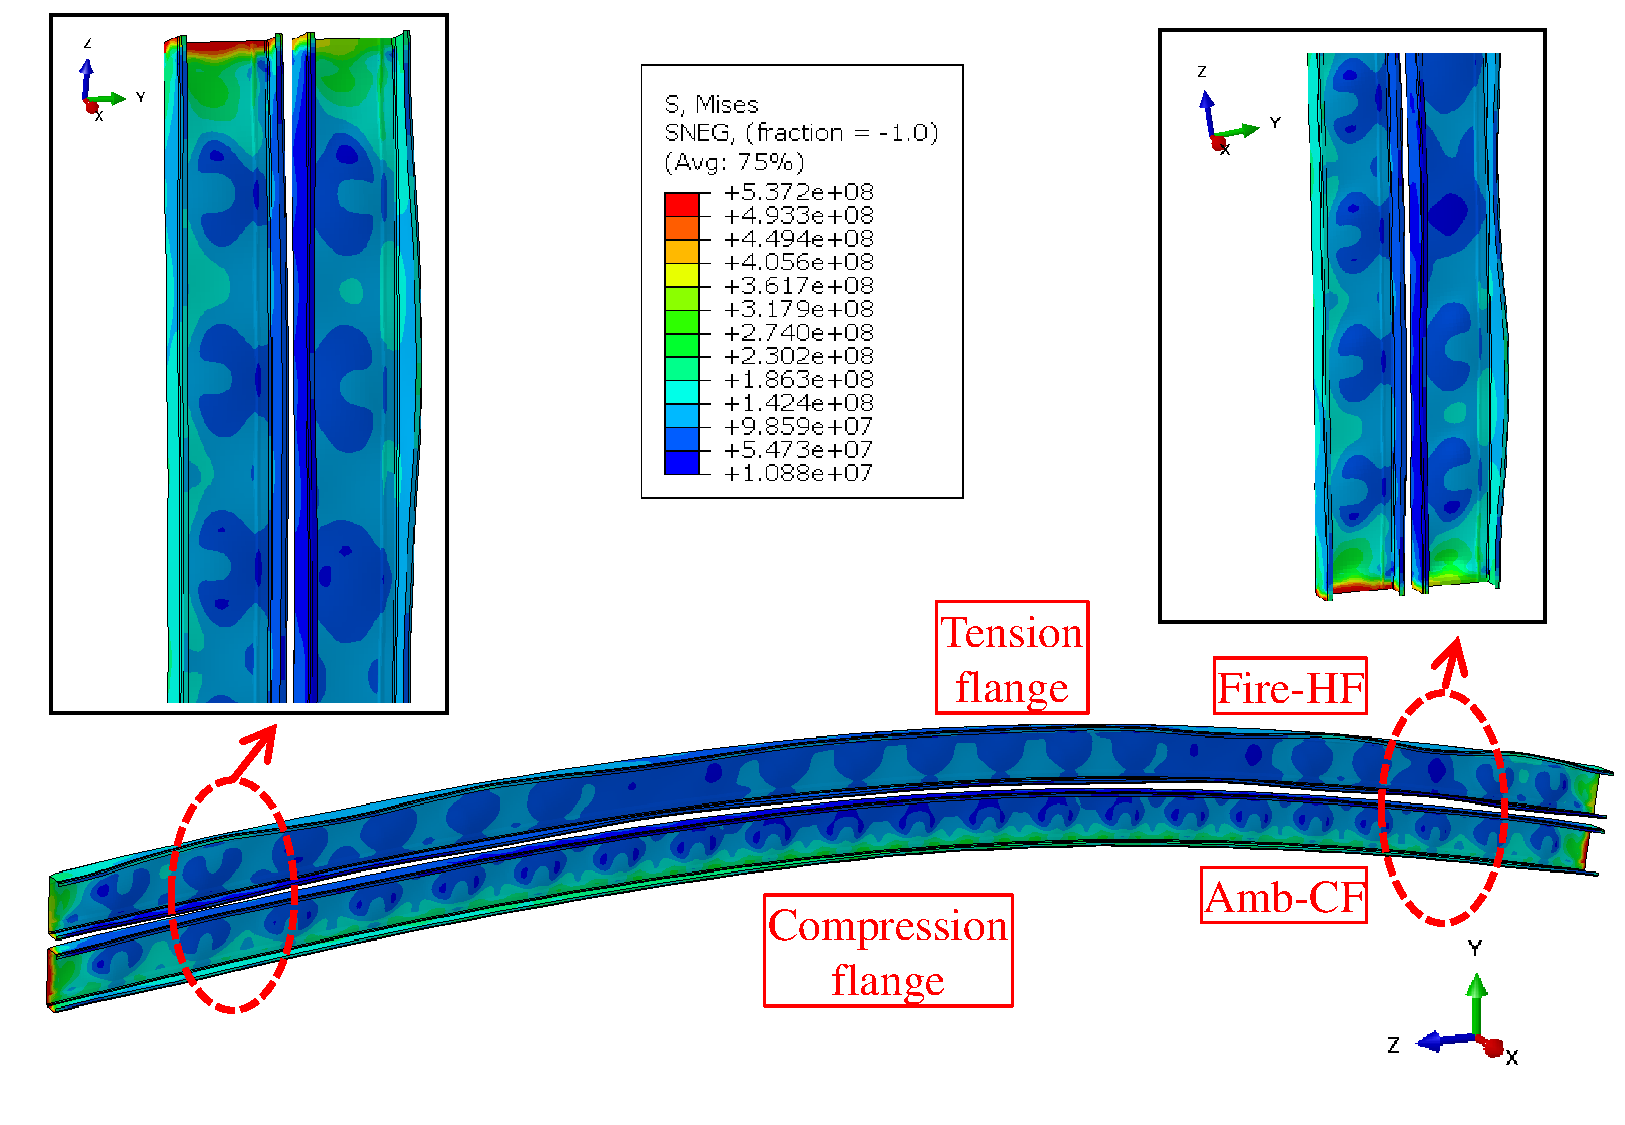
\includegraphics[width=\textwidth]{T1-buckling-FEA.pdf}
		\caption{}
		\label{subfig:T1-buckling-FEA}
	\end{subfigure}
	\begin{subfigure}[b]{0.2\textwidth}
		\centering
		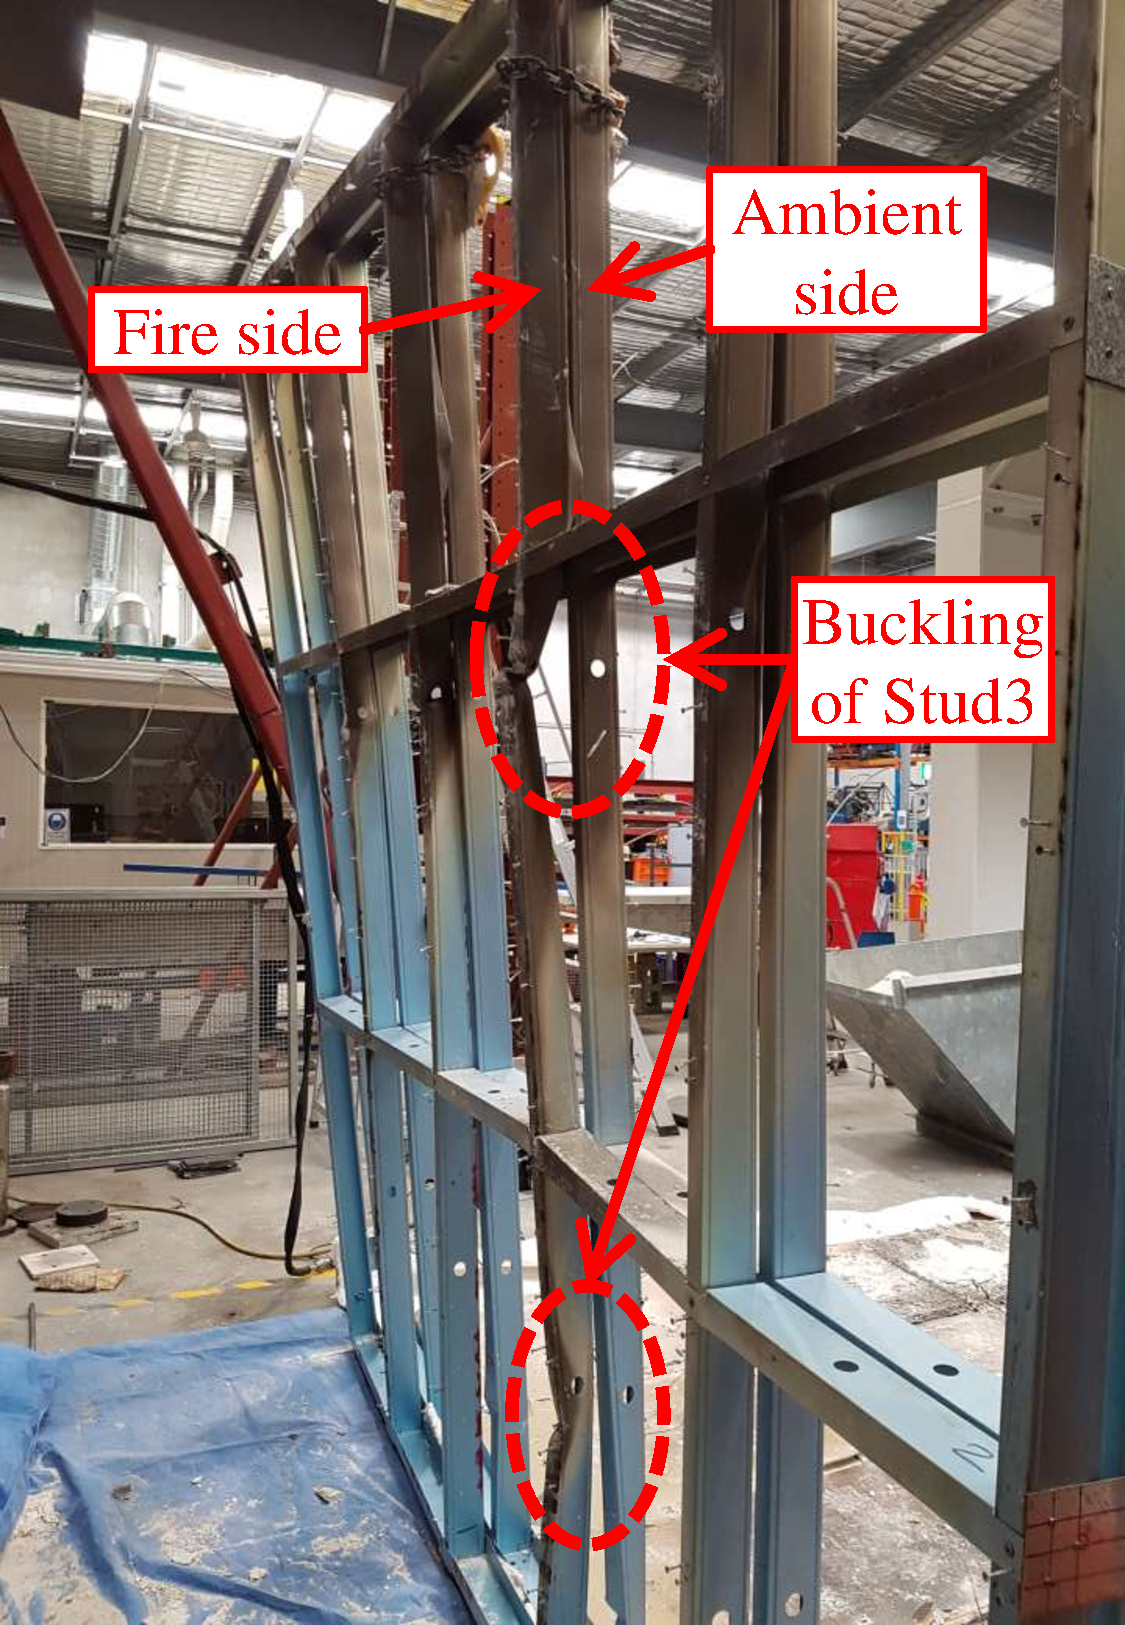
\includegraphics[width=\textwidth]{T1-buckling.pdf}
		\caption{}
		\label{subfig:T1-buckling-FEA-Exp}
	\end{subfigure}
	   \caption{Buckling of studs comparison between FEA and experiment for Test-T1 (a) FEA (b) Experiment}
	   \label{fig:T1-buckling-FE-vs-Exp}
\end{figure} 
\begin{figure}[!htbp]
	\centering
	\begin{subfigure}[b]{0.45\textwidth}
		\centering
		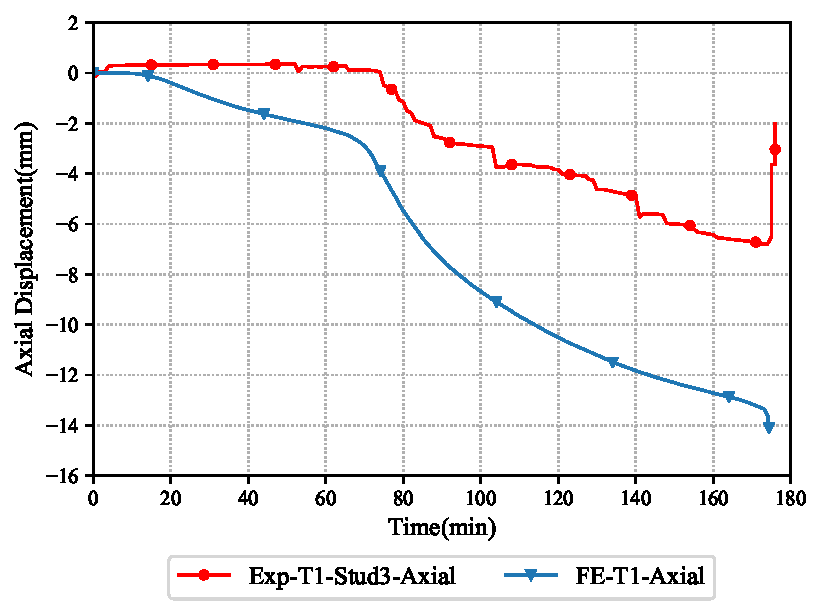
\includegraphics[width=\textwidth]{T1-axial-FE-vs-Exp.pdf}
		\caption{}
		\label{subfig:T1-axial-FE-vs-Exp}
	\end{subfigure}
	\begin{subfigure}[b]{0.45\textwidth}
		\centering
		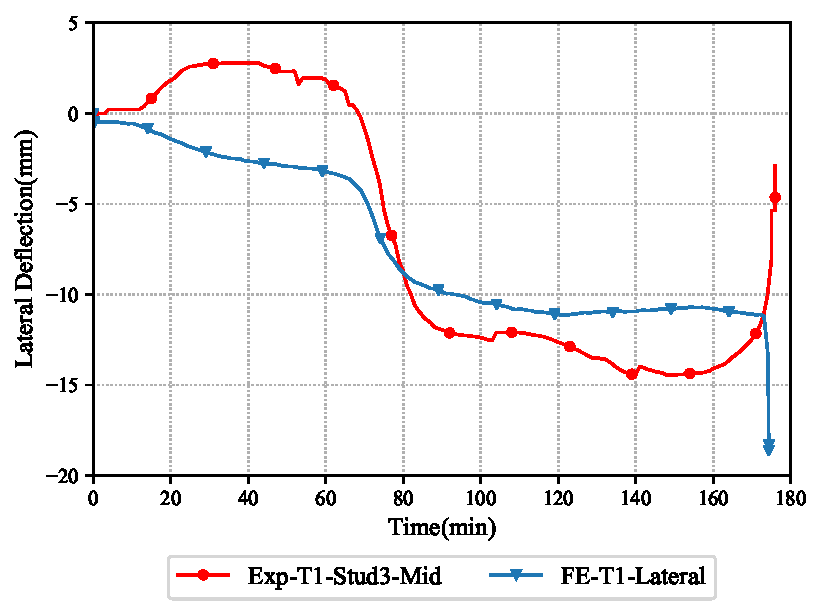
\includegraphics[width=\textwidth]{T1-lateral-FE-vs-Exp.pdf}
		\caption{}
		\label{subfig:T1-lateral-FE-vs-Exp}
	\end{subfigure}
	   \caption{Axial displacement and lateral deflection curves comparison of Test-T1 with FE (a) Axial displacement versus time (b) Lateral deflection versus time curves}
	   \label{fig:T1-structural-FE-vs-Exp}
\end{figure} 

\section*{Test-T2}

Test-T2 was conducted on non-cavity insulated double stud LSF walls similar to the configuration shown in \Cref{fig:T1-plan-FEA} but with thinner studs (90 $\times$ 0.75 mm) under 0.4 LR. The axial compression capacity under ambient temperature conditions resulted in a failure load of 46.25 kN. Structural analysis for Test-T2 was carried out with an axial compression load of 18.5 kN representing 0.4 LR. The axial displacement and lateral deflection versus time curves from FE structural analysis corresponding to Test-T2 are compared against experimental results and is shown in \Cref{fig:T2-structural-FE-vs-Exp}. The axial displacement versus time curve from experiment shows no significant variation for the initial 70 min. However, the predictions from the structural FE model shows a gradual increase in the curve as shown in \Cref{subfig:T2-axial-FE-vs-Exp}. The axial displacement curve is steep after 70 min in both the experimental results and the FE model prediction. Sudden increase in the curve at test failure witnessed in the experimental results could also be predicted by the developed FE structural model. The maximum axial displacement recorded from the experiment was 7.13 mm while it was 13.11 mm from the FE model prediction. \Cref{subfig:T2-lateral-FE-vs-Exp} shows the lateral deflection versus time curves comparison between experimental results and numerical model prediction. The flat region in the lateral deflection curve till 60 min from the experiment was also witnessed in the FE model prediction. However, the maximum lateral deflection reported in the experiment was larger from the experiment resulting -20.25 mm while it was 16.56 mm from the FE model prediction. Failure time from the FE model prediction was 174 min while it was 132 min from the experiment. This difference in failure time prediction is because of the premature plasterboard fall-off in the fire Test-T2 as reported in \Cref{sec:t2-results}.        
\begin{figure}[!htbp]
	\centering
	\begin{subfigure}[b]{0.8\textwidth}
		\centering
		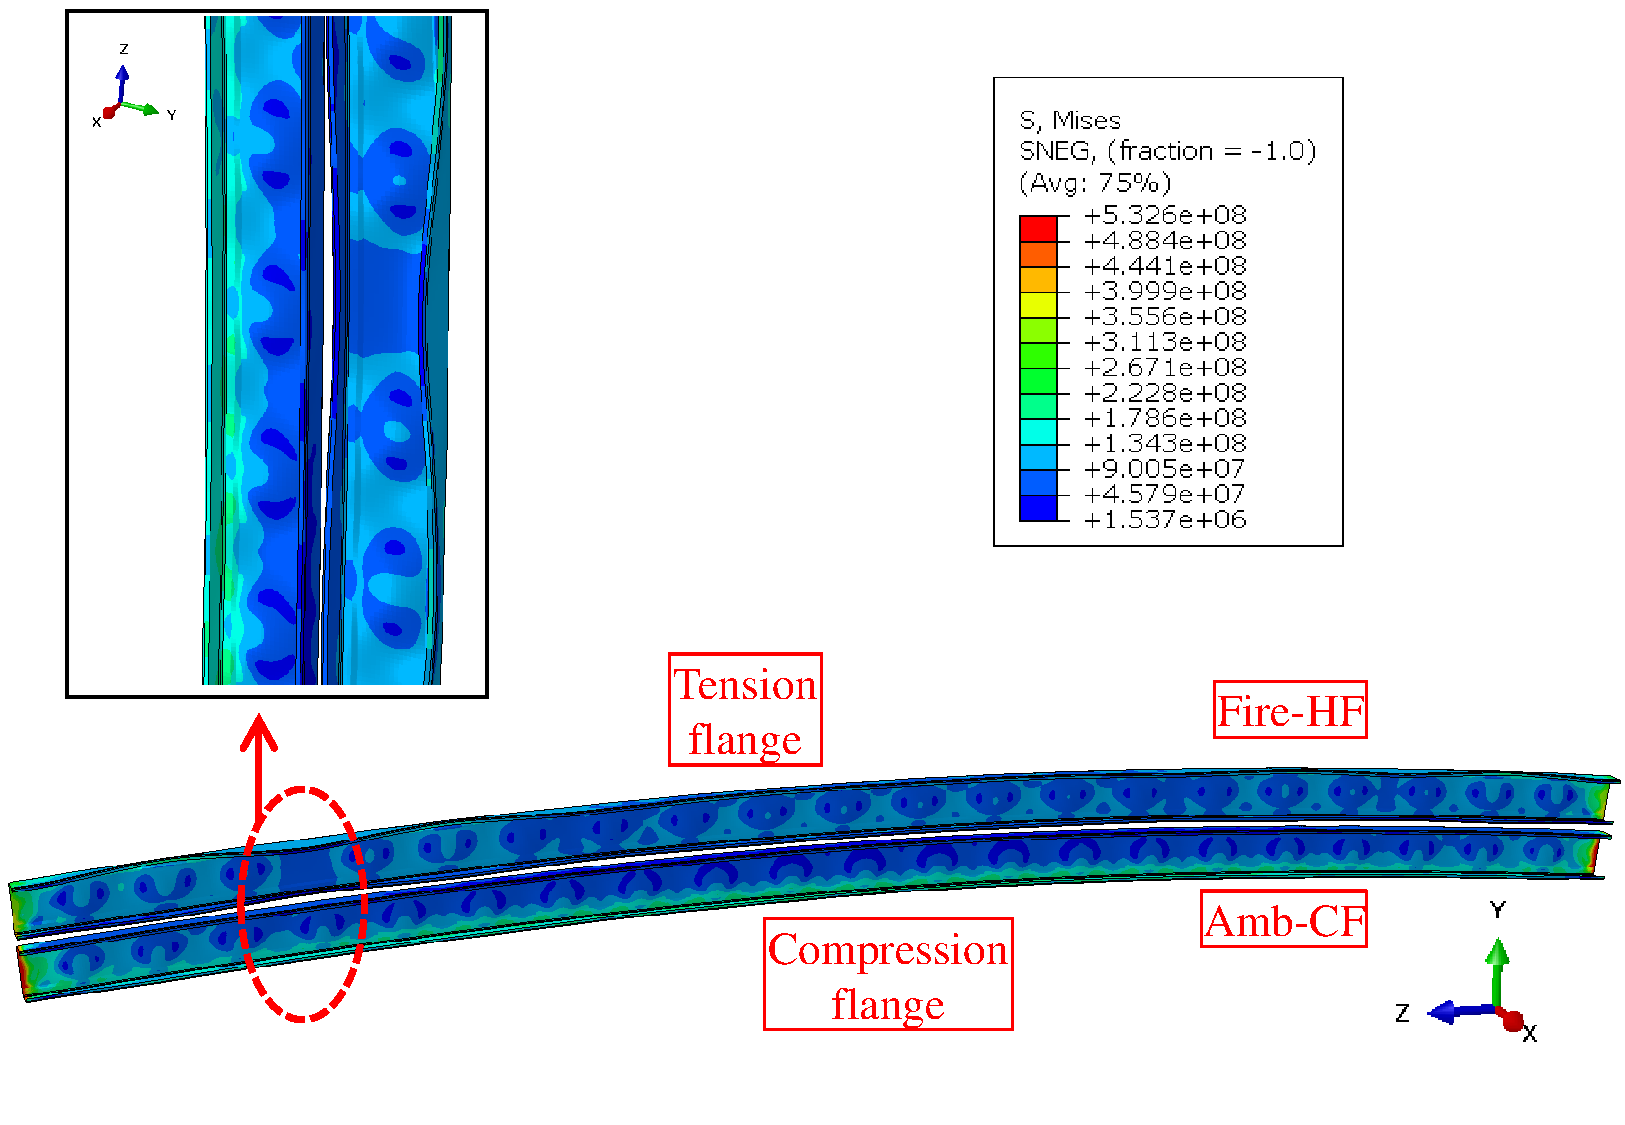
\includegraphics[width=\textwidth]{T2-buckling-FEA.pdf}
		\caption{}
		\label{subfig:T2-buckling-FEA}
	\end{subfigure}
	\begin{subfigure}[b]{0.3\textwidth}
		\centering
		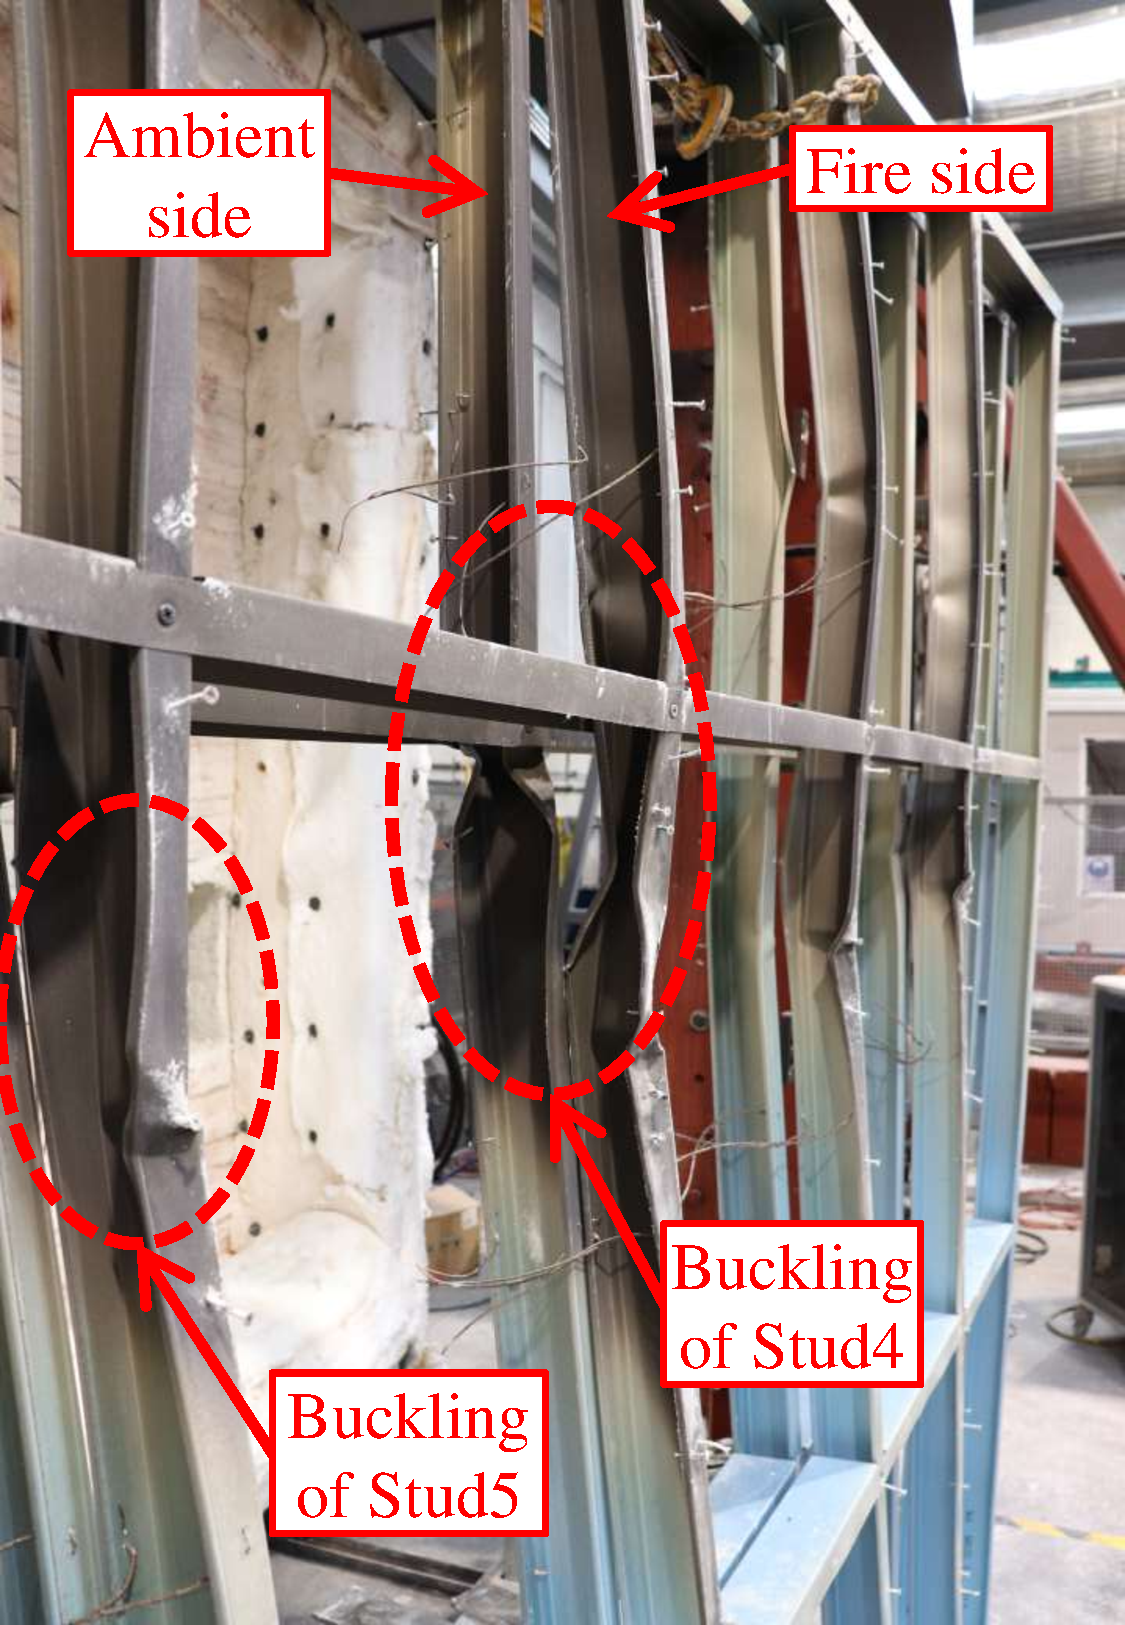
\includegraphics[width=\textwidth]{T2-buckling.pdf}
		\caption{}
		\label{subfig:T2-buckling-FEA-Exp}
	\end{subfigure}
	   \caption{Buckling of studs comparison between FEA and experiment for Test-T2 (a) FEA (b) Experiment}
	   \label{fig:T2-buckling-FE-vs-Exp}
\end{figure} 
\begin{figure}[!htbp]
	\centering
	\begin{subfigure}[b]{0.45\textwidth}
		\centering
		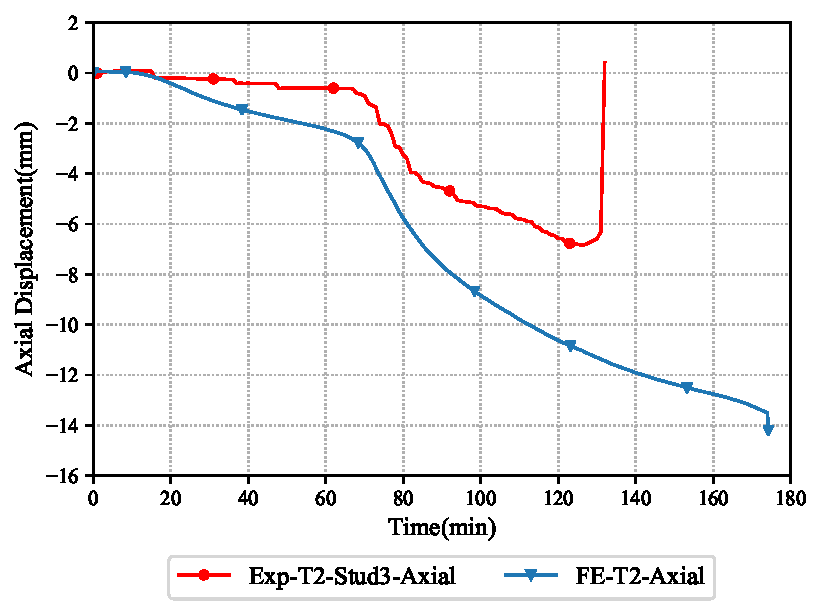
\includegraphics[width=\textwidth]{T2-axial-FE-vs-Exp.pdf}
		\caption{}
		\label{subfig:T2-axial-FE-vs-Exp}
	\end{subfigure}
	\begin{subfigure}[b]{0.45\textwidth}
		\centering
		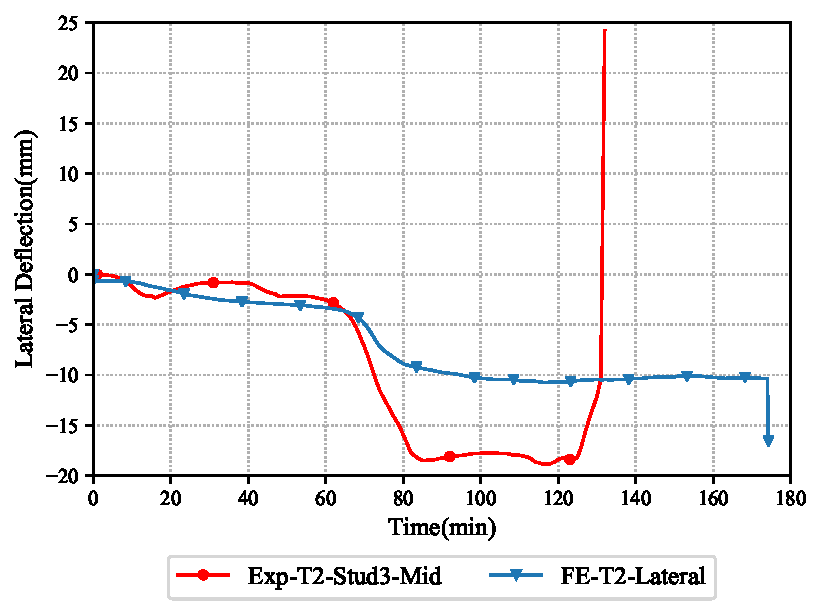
\includegraphics[width=\textwidth]{T2-lateral-FE-vs-Exp.pdf}
		\caption{}
		\label{subfig:T2-lateral-FE-vs-Exp}
	\end{subfigure}
	   \caption{Axial displacement and lateral deflection curves comparison of Test-T2 with FE (a) Axial displacement versus time (b) Lateral deflection versus time curves}
	   \label{fig:T2-structural-FE-vs-Exp}
\end{figure} 

\section*{Test-T3}

Test-T3 was conducted on non-cavity insulated double stud LSF walls similar to the configuration shown in \Cref{fig:T1-plan-FEA} with 90 $\times$ 0.75 mm studs but under a higher load ratio of 0.6 LR. The axial displacement and lateral deflection versus time curves between FE model prediction and experimental results are shown in \Cref{fig:T3-structural-FE-vs-Exp}. The gradual increase in slope exhibited by the axial displacement curve from experiment was also noticeable in the FE predictions as shown in \Cref{subfig:T3-axial-FE-vs-Exp}. The lateral deflection was nearly flat and reaching a sudden increase at the end of fire test. This behaviour in the lateral deflection could also be predicted by the structural FE model as shown in \Cref{subfig:T3-lateral-FE-vs-Exp}. The failure time predicted by the FE model was 82 min while the experiment resulted a failure time of 81 min. The agreement in failure time between the FE model prediction and experimental result was reasonable in Test-T3 as no significant plasterboard fall-off was noticeable in the full-scale fire test unlike Test-T2.
\begin{figure}[!htbp]
	\centering
	\begin{subfigure}[b]{0.8\textwidth}
		\centering
		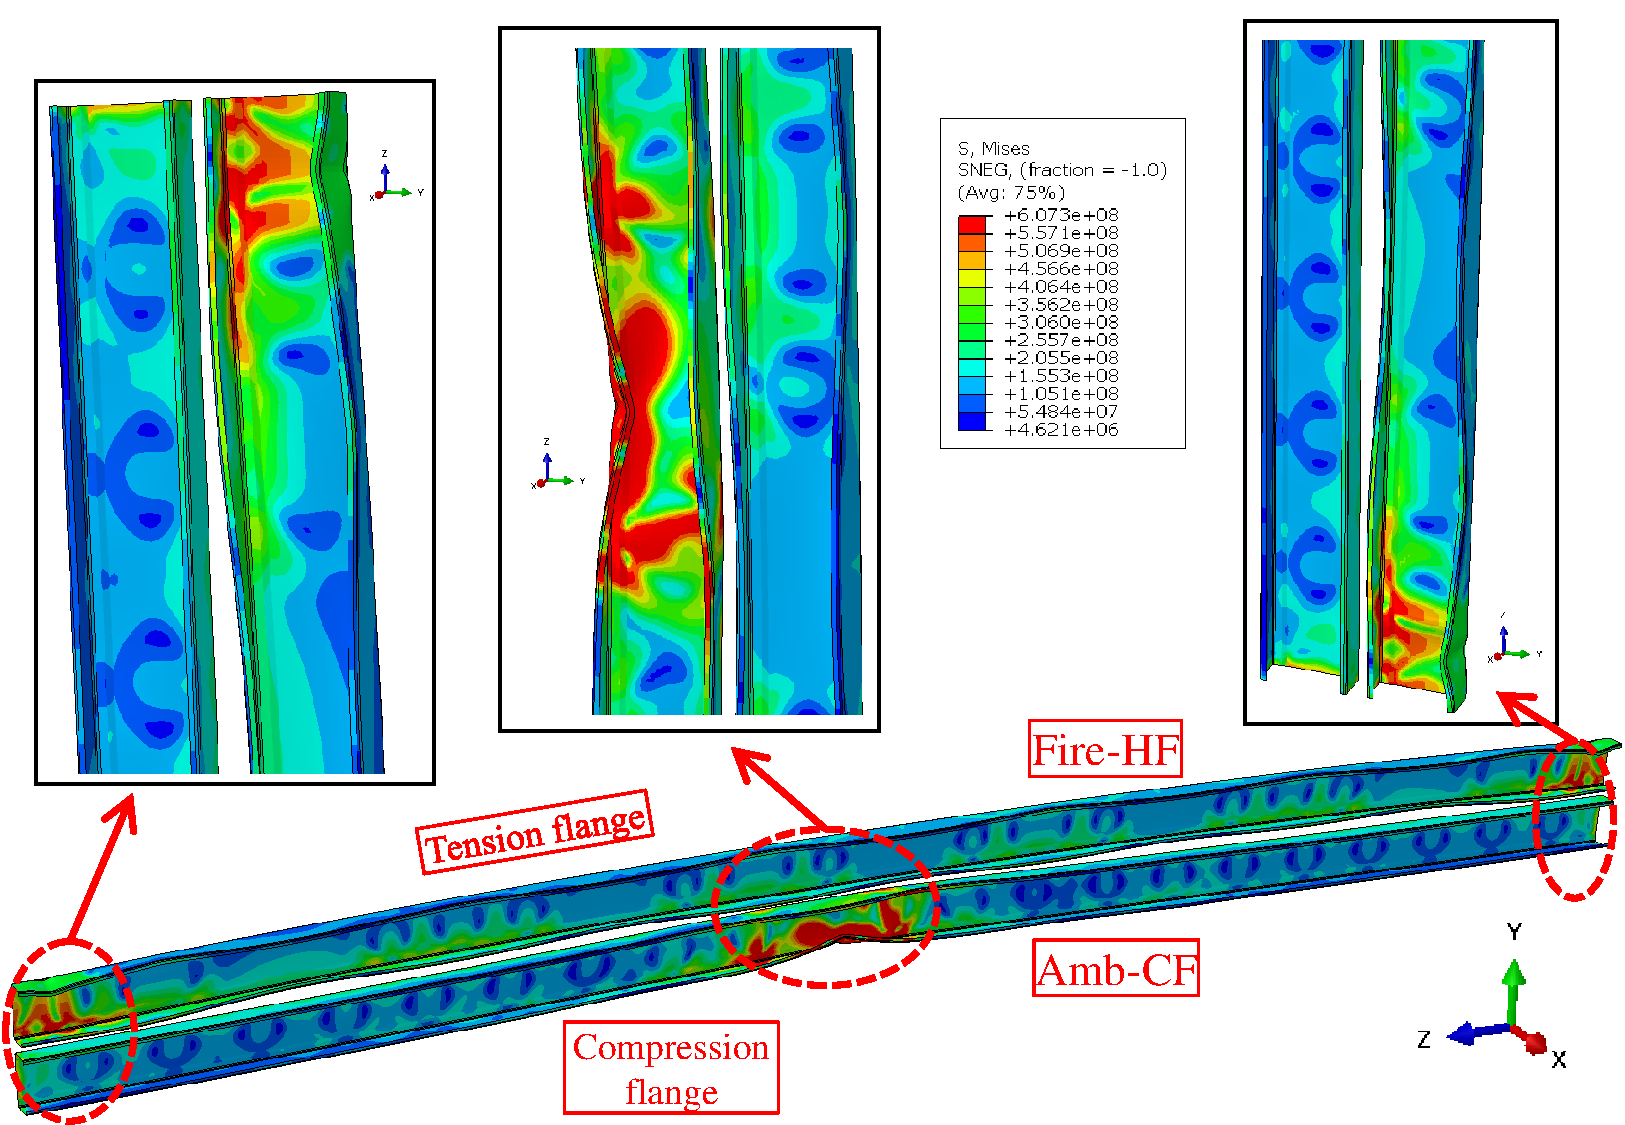
\includegraphics[width=\textwidth]{T3-buckling-FEA.pdf}
		\caption{}
		\label{subfig:T3-buckling-FEA}
	\end{subfigure}
	\begin{subfigure}[b]{0.3\textwidth}
		\centering
		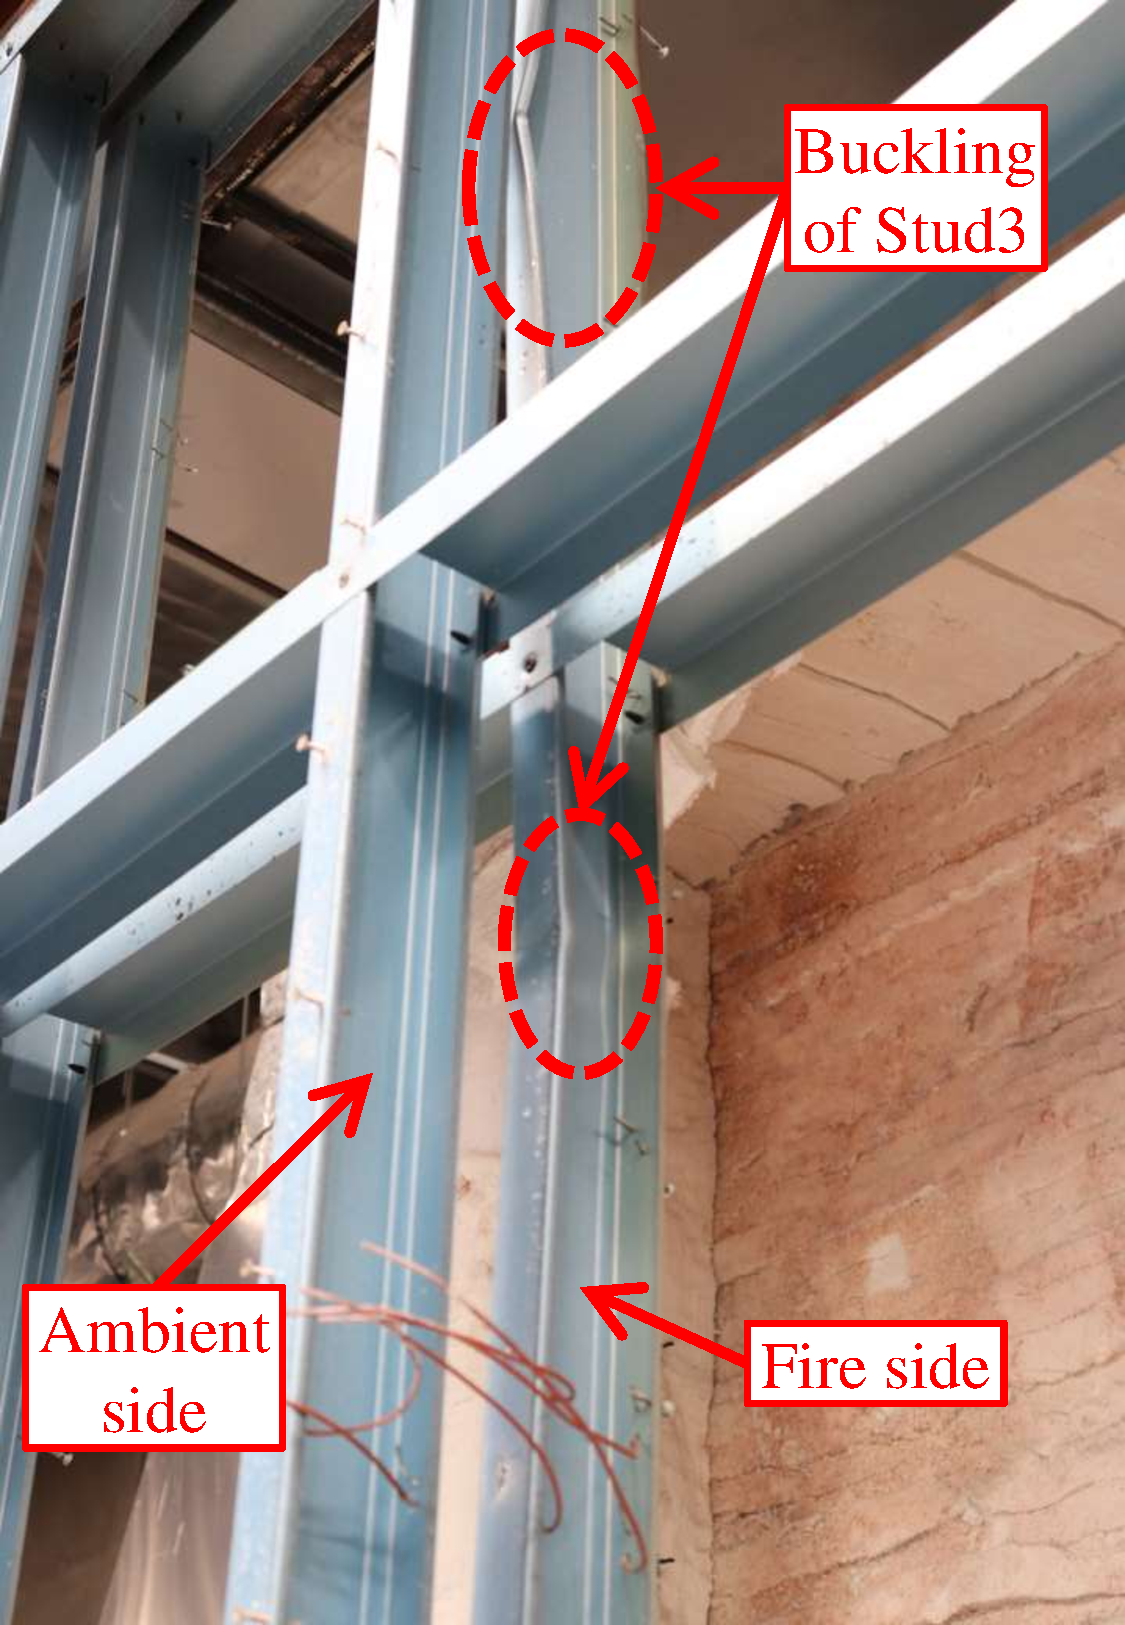
\includegraphics[width=\textwidth]{T3-buckling.pdf}
		\caption{}
		\label{subfig:T3-buckling-FEA-Exp}
	\end{subfigure}
	   \caption{Buckling of studs comparison between FEA and experiment for Test-T3 (a) FEA (b) Experiment}
	   \label{fig:T3-buckling-FE-vs-Exp}
\end{figure} 
\begin{figure}[!htbp]
	\centering
	\begin{subfigure}[b]{0.45\textwidth}
		\centering
		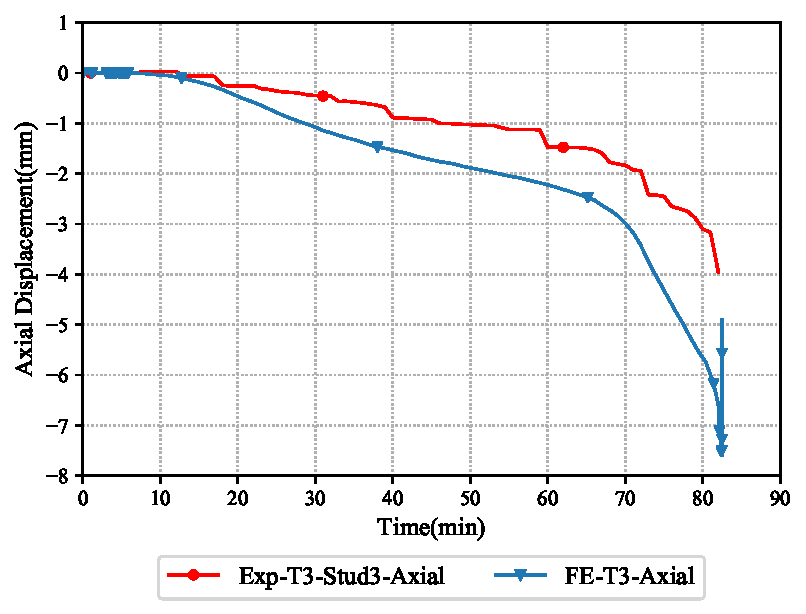
\includegraphics[width=\textwidth]{T3-axial-FE-vs-Exp.pdf}
		\caption{}
		\label{subfig:T3-axial-FE-vs-Exp}
	\end{subfigure}
	\begin{subfigure}[b]{0.45\textwidth}
		\centering
		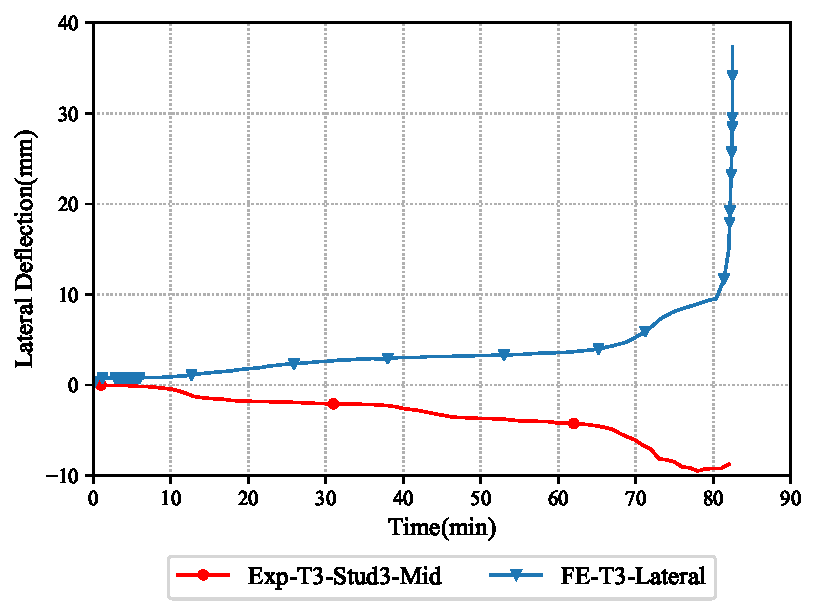
\includegraphics[width=\textwidth]{T3-lateral-FE-vs-Exp.pdf}
		\caption{}
		\label{subfig:T3-lateral-FE-vs-Exp}
	\end{subfigure}
	   \caption{Axial displacement and lateral deflection curves comparison of Test-T3 with FE (a) Axial displacement versus time (b) Lateral deflection versus time curves}
	   \label{fig:T3-structural-FE-vs-Exp}
\end{figure} 

\section*{Test-T4}

Test-T4 was conducted on non-cavity insulated double stud LSF walls with 70 $\times$ 0.95 mm studs based on the configuration shown in \Cref{fig:T4-plan-FEA}. The axial displacement and lateral deflection versus time curves from experiment and FE predictions are compared against each other and is shown in \Cref{fig:T4-structural-FE-vs-Exp}. The axial displacement versus time curve from the experiment as shown in \Cref{subfig:T4-axial-FE-vs-Exp} exhibited a flat region till 60 min of fire test after which it progressively increased to a maximum of -5.95 mm at the end of fire test. This behaviour was also reflected in the structural FE model prediction wherein a maximum axial displacement of 15 mm was recorded at the end of fire test. The axial displacement versus time curve then changed sign indicating structural failure in the model similar to the experiment. 
\begin{figure}[!htbp]
	\centering
			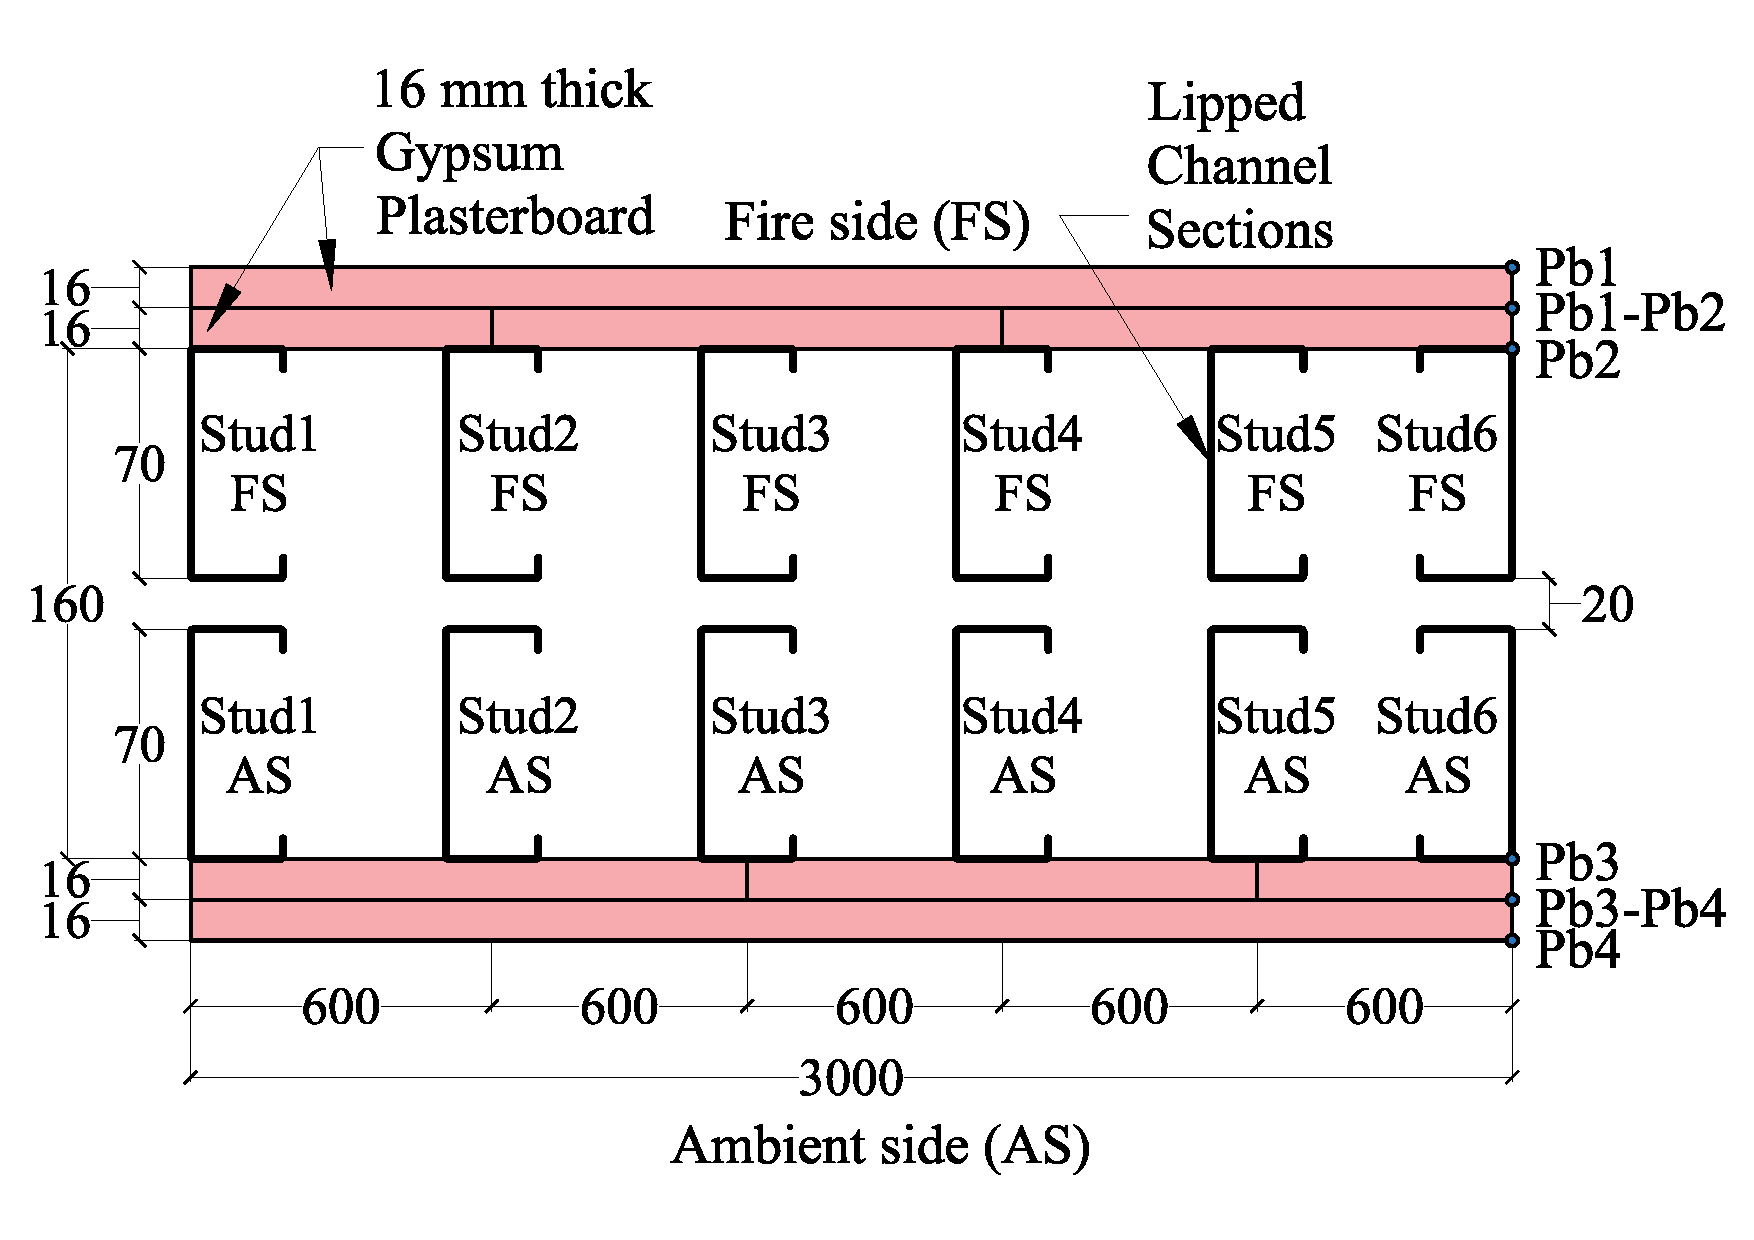
\includegraphics[scale=0.2]{T4-plan.pdf}\\
		\caption{Test-T4 plan view}
		\label{fig:T4-plan-FEA}
\end{figure}Lateral deflection versus time curve shown in \Cref{subfig:T4-lateral-FE-vs-Exp} also exhibited reasonable agreement between the FE model prediction and the experimental result. The change in slope experienced in the lateral deflection versus time curve after 60 min was also reflected in the FE model prediction. The maximum lateral deflection predicted by the FE model at the time of failure was 19 mm while it was -24.43 mm from the experiment. The failure time predicted by the FE model was 178 min while it was 171 min from the experiment. Local compressive failure on the fire side hot flange of studs experienced in the full-scale fire test could also be simulated by the developed FE model as shown in \Cref{fig:T4-buckling-FE-vs-Exp}. It is to note that the axial compression load given to the structural FE model was based on the predictions from \Cref{ch:Ambient} where the ambient compression capacity predicted by the ambient structural model was less than the ambient capacity experimental result. When the non-dimensional load ratio is taken for consideration, the failure time prediction for the full-scale fire test matched reasonably well with the experimental failure time of Test-T4.   
\begin{figure}[!htbp]
	\centering
	\begin{subfigure}[b]{0.8\textwidth}
		\centering
		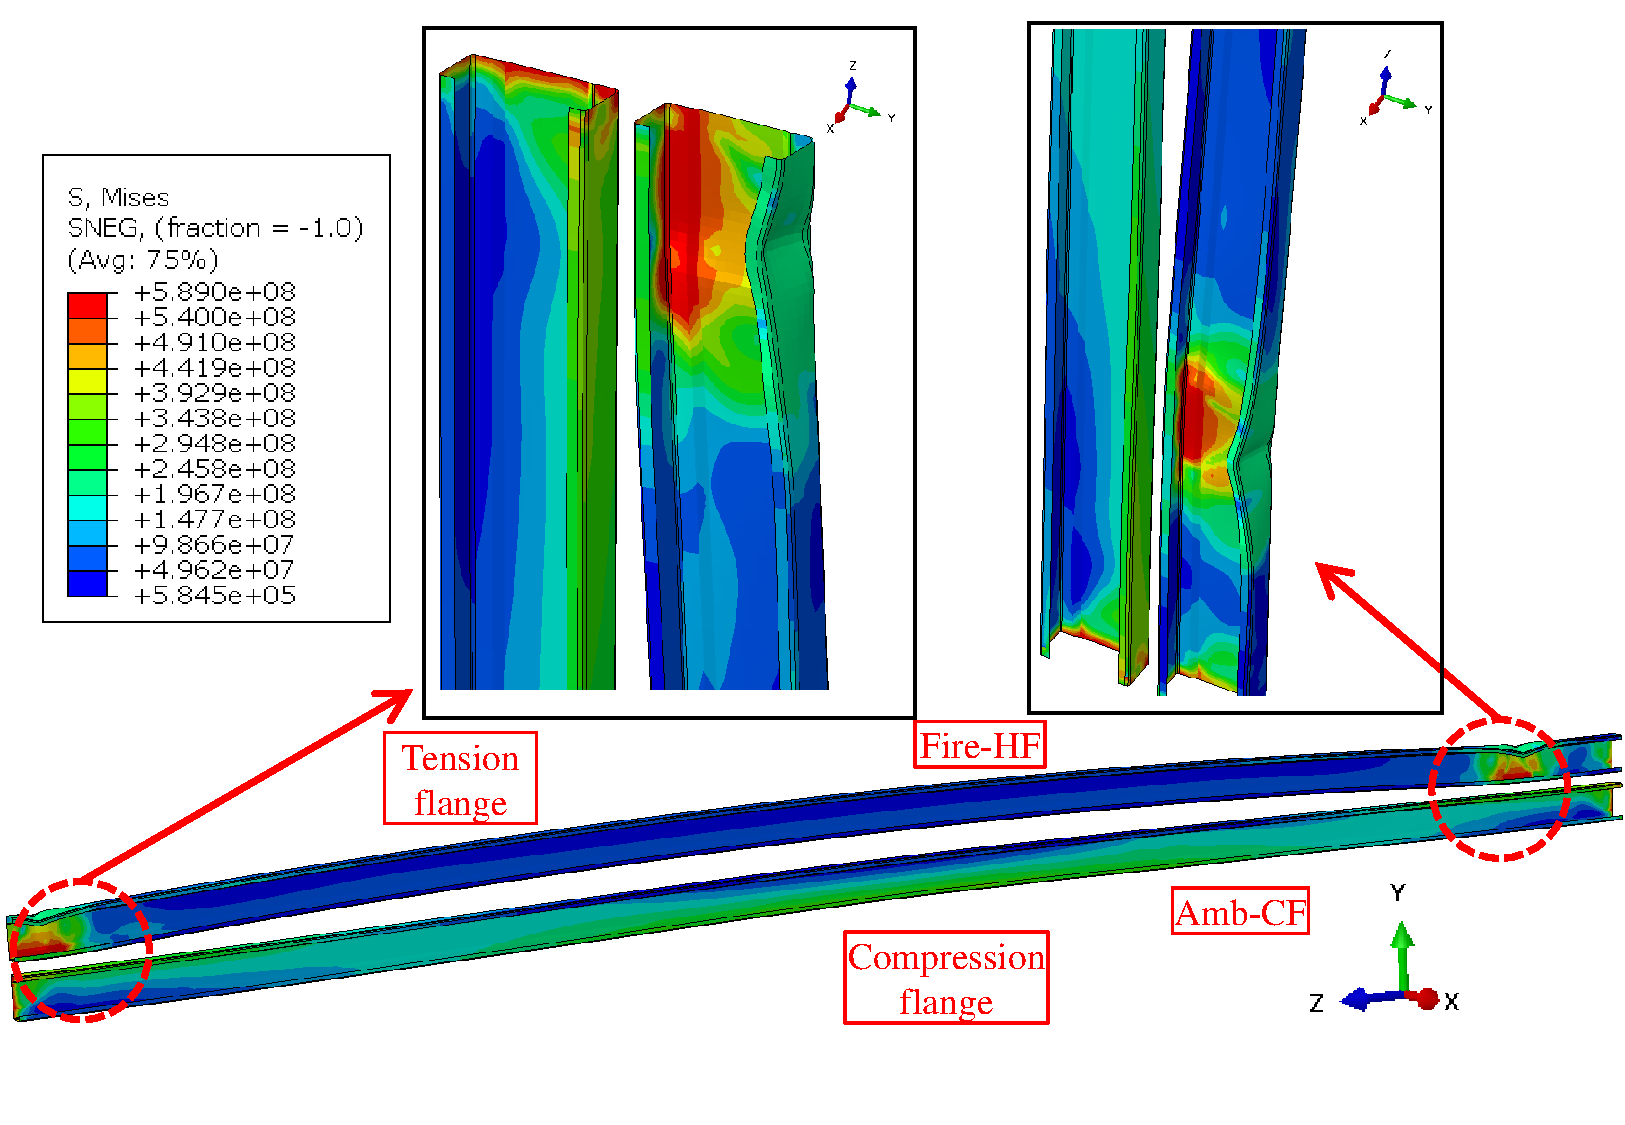
\includegraphics[width=\textwidth]{T4-buckling-FEA.pdf}
		\caption{}
		\label{subfig:T4-buckling-FEA}
	\end{subfigure}
	\begin{subfigure}[b]{0.3\textwidth}
		\centering
		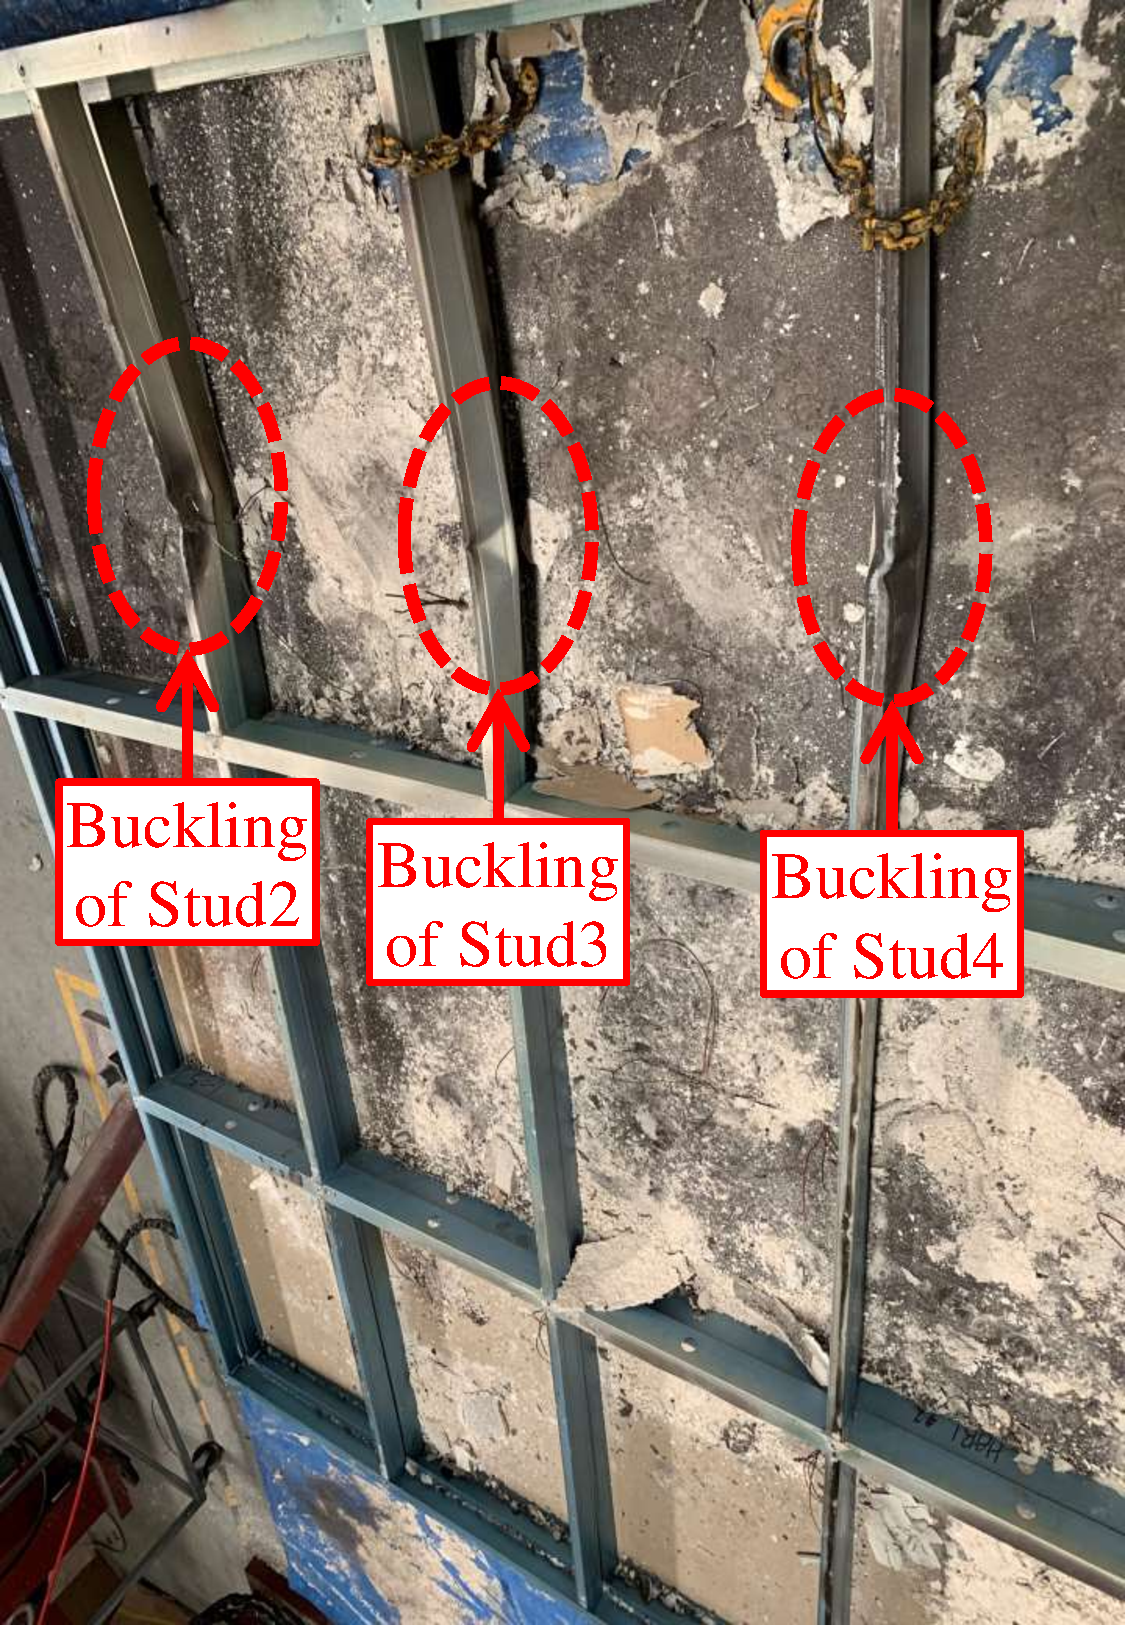
\includegraphics[width=\textwidth]{T4-buckling.pdf}
		\caption{}
		\label{subfig:T4-buckling-FEA-Exp}
	\end{subfigure}
	   \caption{Buckling of studs comparison between FEA and experiment for Test-T4 (a) FEA (b) Experiment}
	   \label{fig:T4-buckling-FE-vs-Exp}
\end{figure} 
\begin{figure}[!htbp]
	\centering
	\begin{subfigure}[b]{0.45\textwidth}
		\centering
		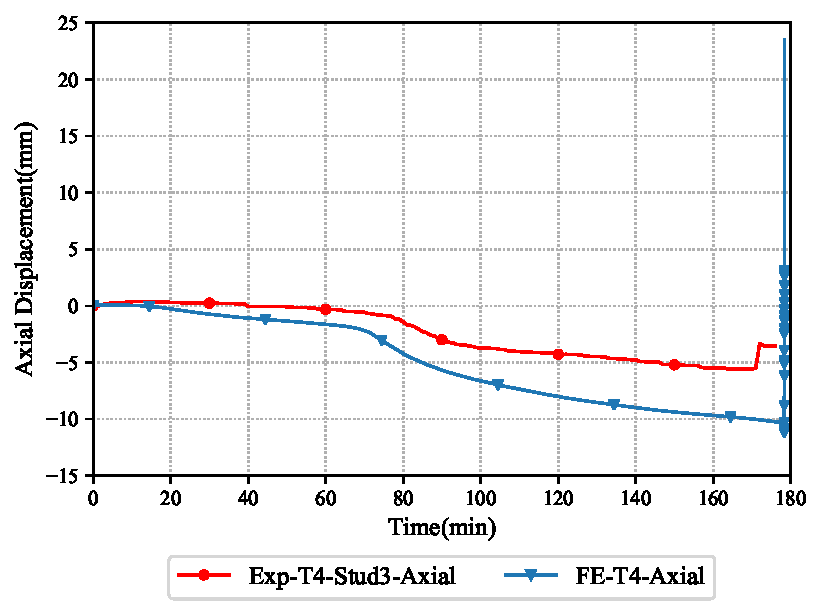
\includegraphics[width=\textwidth]{T4-axial-FE-vs-Exp.pdf}
		\caption{}
		\label{subfig:T4-axial-FE-vs-Exp}
	\end{subfigure}
	\begin{subfigure}[b]{0.45\textwidth}
		\centering
		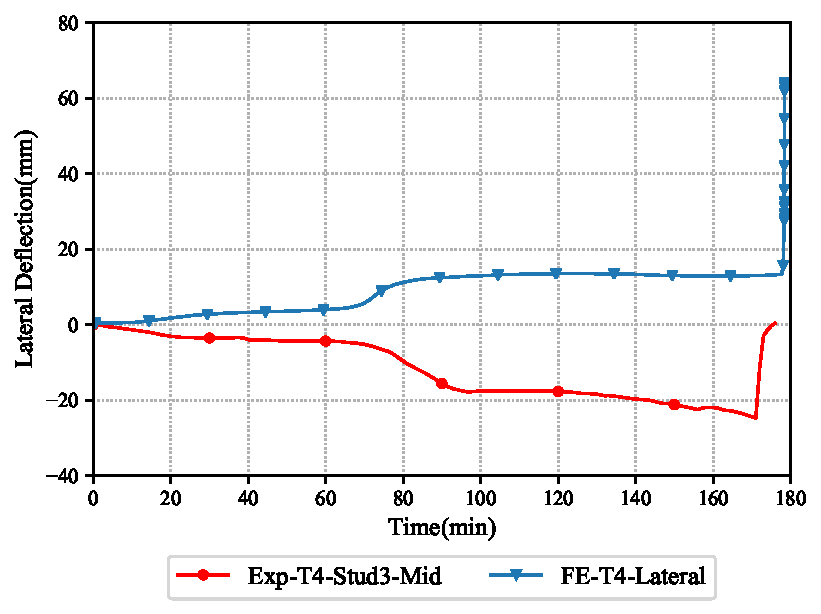
\includegraphics[width=\textwidth]{T4-lateral-FE-vs-Exp.pdf}
		\caption{}
		\label{subfig:T4-lateral-FE-vs-Exp}
	\end{subfigure}
	   \caption{Axial displacement and lateral deflection curves comparison of Test-T4 with FE (a) Axial displacement versus time (b) Lateral deflection versus time curves}
	   \label{fig:T4-structural-FE-vs-Exp}
\end{figure}

\section*{Test-T5}

Test-T5 was conducted double stud LSF walls with glass fibre cavity insulation and 90 $\times$ 0.95 mm studs as shown on \Cref{fig:T5-plan-FEA}. The difference between the cavity insulated wall tests in comparison with the non-cavity insulated wall tests is the large temperature difference between the hot and cold flanges. This was also predicted by the developed FDS thermal model as discussed in \Cref{ch:FE-Thermal}, \Cref{sec:fds-cavity-models}. The input boundary conditions of the structural FE models also incorporated these effects. The axial displacement and lateral deflection versus time curves from the structural FE analysis are compared against the experimental results and is presented in \Cref{fig:T5-structural-FE-vs-Exp}. similar to the experimental results the axial displacement versus time curve shown in \Cref{subfig:T5-axial-FE-vs-Exp} was flat till the end of the fire test simulation. 

The maximum axial displacement was 5 mm from the FE model prediction, while it was -1.55 mm in the experiment. Similar trend was observed in the lateral deflection versus time curve comparison shown in \Cref{subfig:T5-lateral-FE-vs-Exp}. The lateral deflection versus time curve was flat in both the FE model prediction and experiment. Maximum lateral deflection at before the failure time was -11.35 mm in the experiment while it was -16.87 mm in the FE model prediction. However, the flat region in the lateral deflection curve was similar in both the FE model prediction and the experiment. This is in correlation with the earlier finding from the experimental study in \Cref{ch:Fire} that the lateral deflection due to thermal bowing is less in cavity insulated double stud LSF walls in comparison with the non-cavity insulated double stud walls. The failure time predicted by the FE model was 80 min while it was 76 min from the experiment.  
\begin{figure}[!htbp]
	\centering
			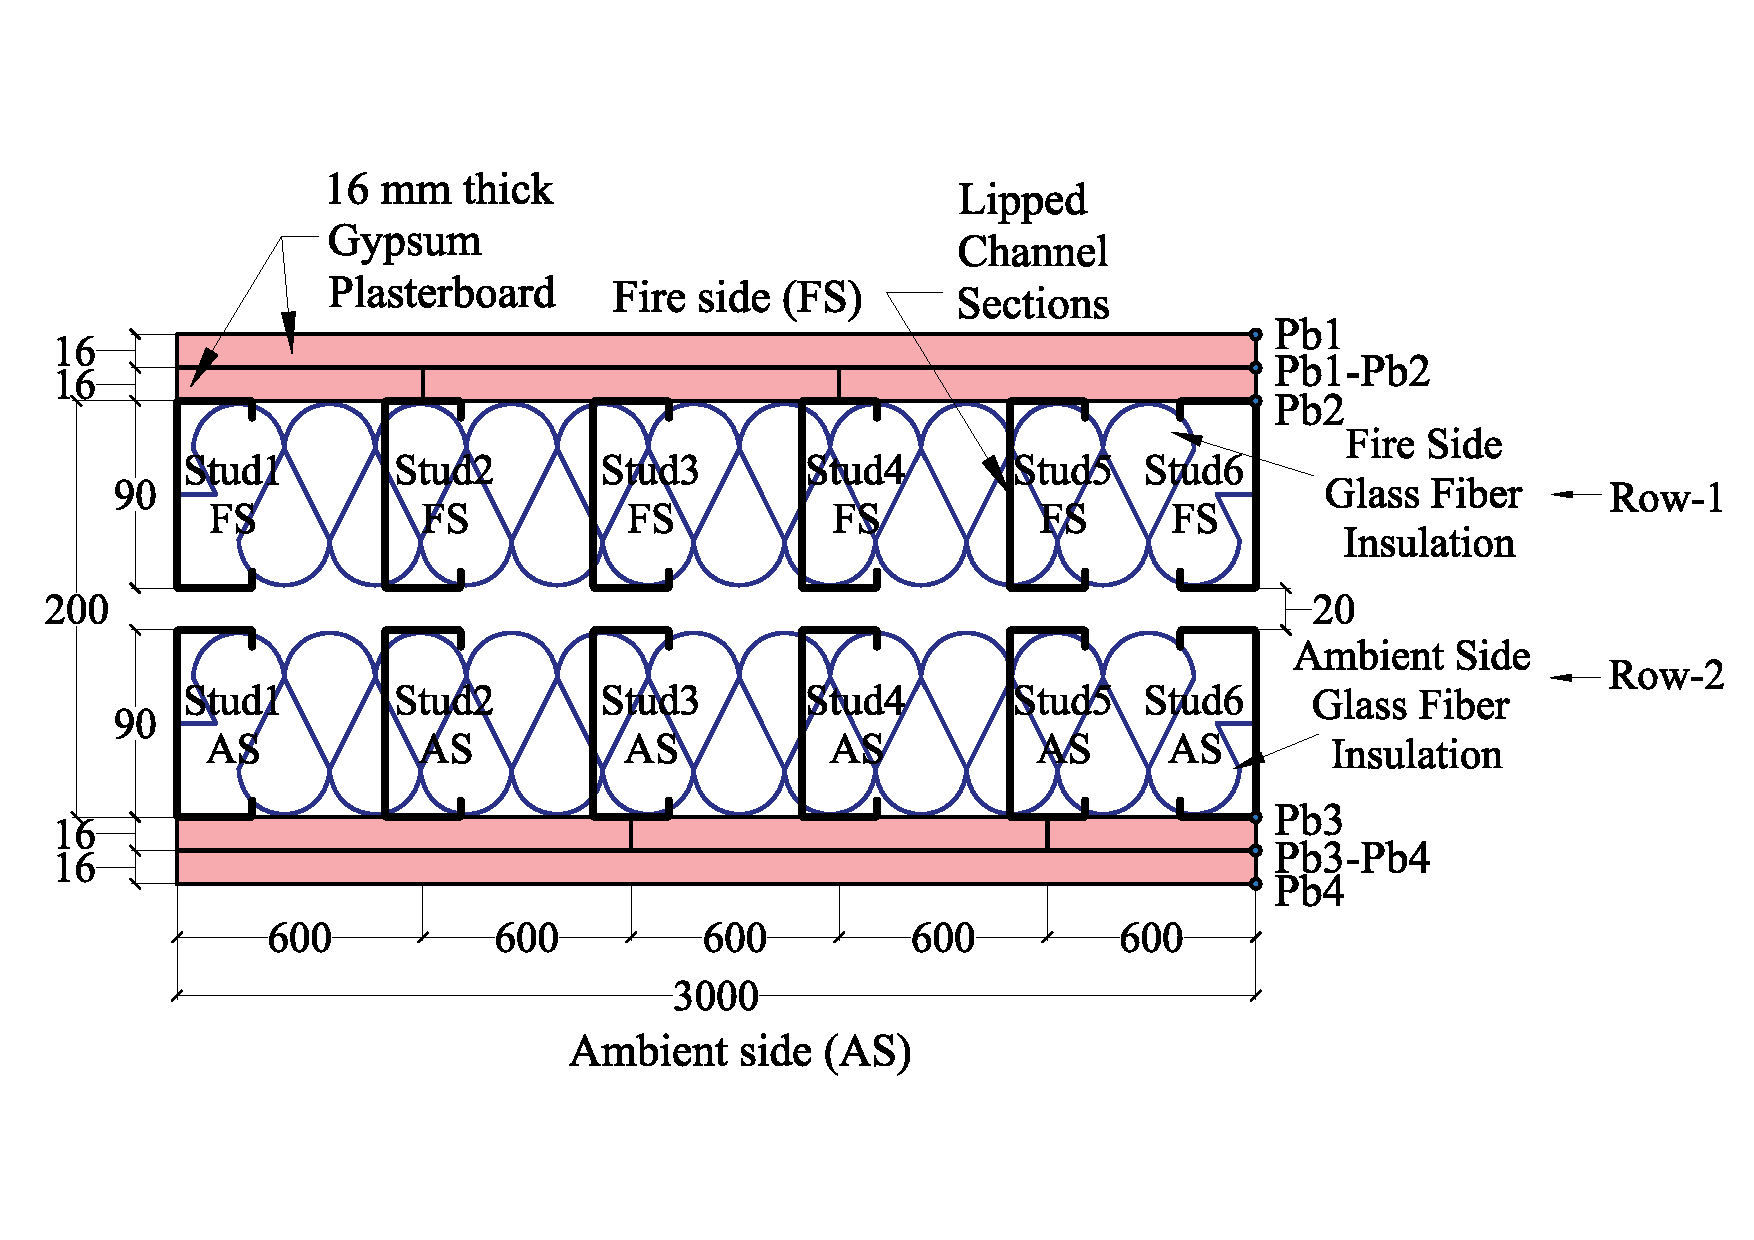
\includegraphics[scale=0.25]{T5-plan.pdf}\\
		\caption{Test-T5 plan view}
		\label{fig:T5-plan-FEA}
\end{figure}
\begin{figure}[!htbp]
	\centering
	\begin{subfigure}[b]{0.8\textwidth}
		\centering
		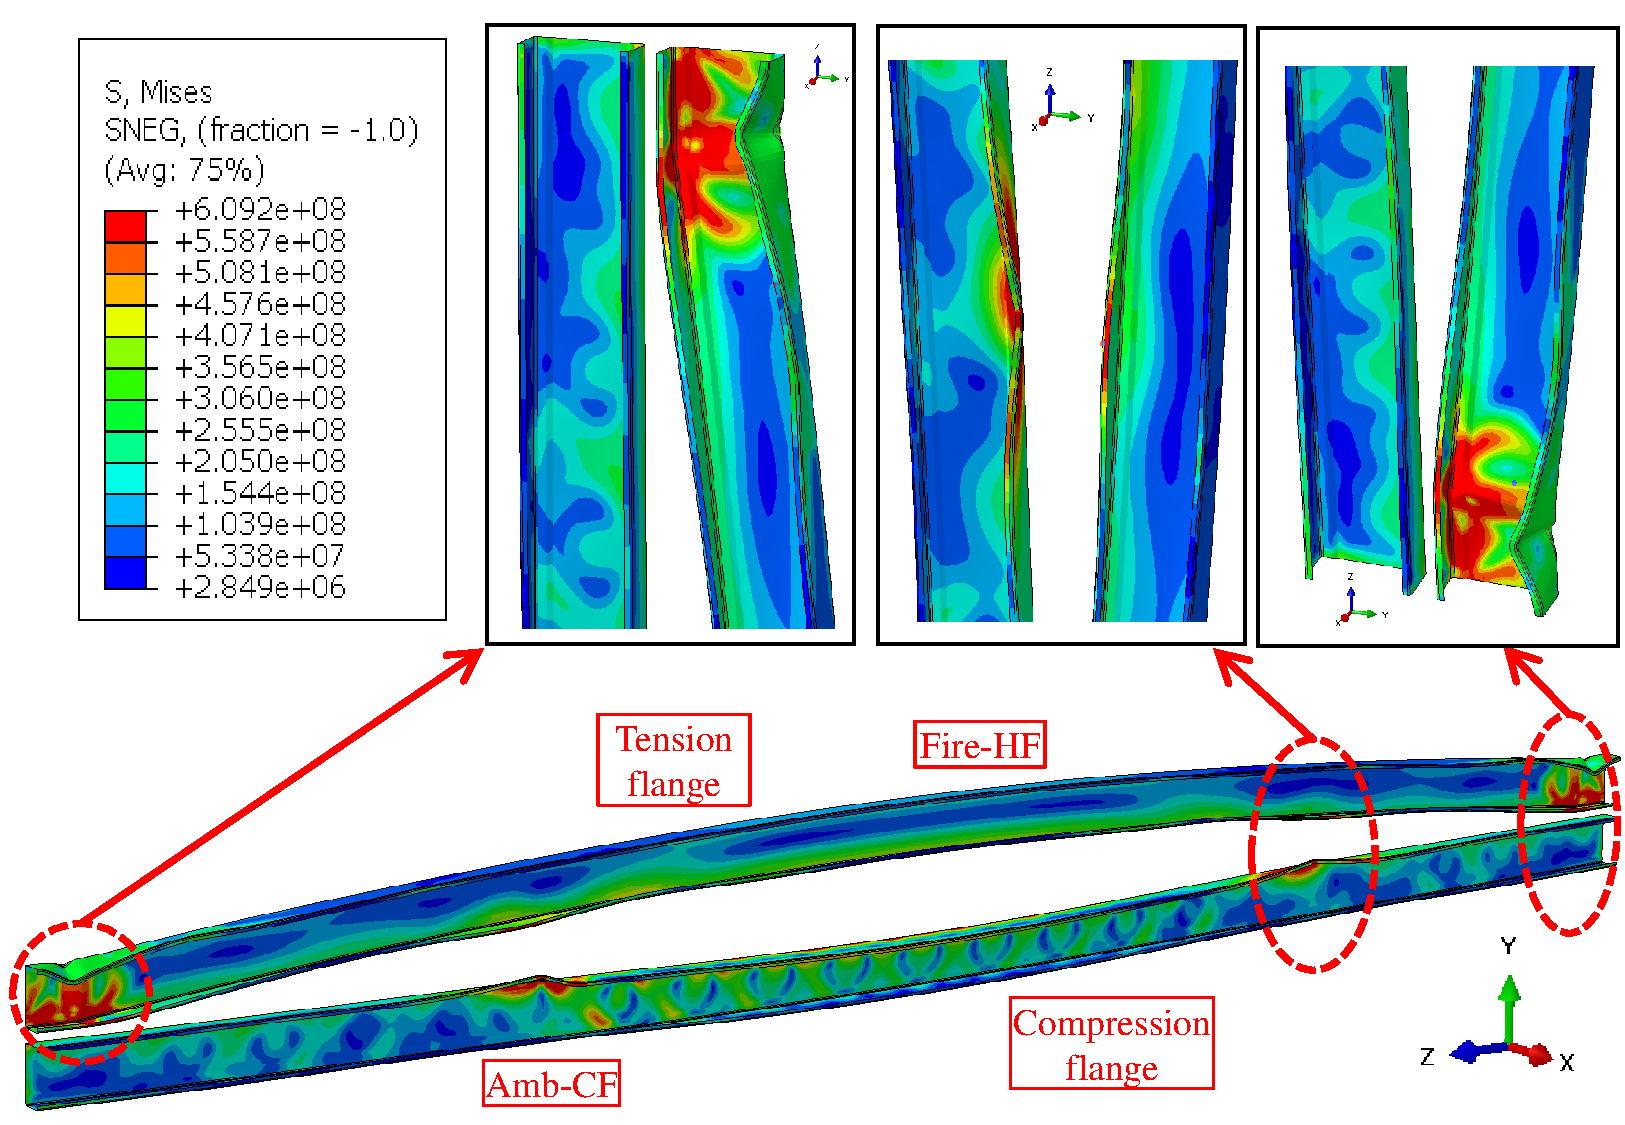
\includegraphics[width=\textwidth]{T5-buckling-FEA.pdf}
		\caption{}
		\label{subfig:T5-buckling-FEA}
	\end{subfigure}
	\begin{subfigure}[b]{0.3\textwidth}
		\centering
		\includegraphics[width=\textwidth]{T5-buckling.pdf}
		\caption{}
		\label{subfig:T5-buckling-FEA-Exp}
	\end{subfigure}
	   \caption{Buckling of studs comparison between FEA and experiment for Test-T5 (a) FEA (b) Experiment}
	   \label{fig:T5-buckling-FE-vs-Exp}
\end{figure} 
\begin{figure}[!htbp]
	\centering
	\begin{subfigure}[b]{0.45\textwidth}
		\centering
		\includegraphics[width=\textwidth]{T5-axial-FE-vs-Exp.pdf}
		\caption{}
		\label{subfig:T5-axial-FE-vs-Exp}
	\end{subfigure}
	\begin{subfigure}[b]{0.45\textwidth}
		\centering
		\includegraphics[width=\textwidth]{T5-lateral-FE-vs-Exp.pdf}
		\caption{}
		\label{subfig:T5-lateral-FE-vs-Exp}
	\end{subfigure}
	   \caption{Axial displacement and lateral deflection curves comparison of Test-T5 with FE (a) Axial displacement versus time (b) Lateral deflection versus time curves}
	   \label{fig:T5-structural-FE-vs-Exp}
\end{figure} 

\section*{Test-T6}

Test-T6 was conducted as a repeat test to that of Test-T5 on cavity insulated double stud LSF walls. Therefore, the same structural FE model was used for the comparison. The experiment resulted a failure time of 91 min while the FE model resulted a failure time of 80 min. The axial displacement and lateral deflection comparison between the FE model and the experimental results are shown in \Cref{fig:T6-structural-FE-vs-Exp}. Similar trend in the axial displacement and lateral deflection versus time curves were observed between the FE model prediction and the experimental results. However, the failure time prediction from the FE model was lower in comparison with the experimental result for Test-T6. However, the difference is failure time prediction is small and can be neglected.      
\begin{figure}[!htbp]
	\centering
	\begin{subfigure}[b]{0.85\textwidth}
		\centering
		\includegraphics[width=\textwidth]{T5-buckling-FEA.pdf}
		\caption{}
		\label{subfig:T6-buckling-FEA}
	\end{subfigure}
	\begin{subfigure}[b]{0.35\textwidth}
		\centering
		\includegraphics[width=\textwidth]{T6-buckling.pdf}
		\caption{}
		\label{subfig:T6-buckling-FEA-Exp}
	\end{subfigure}
	   \caption{Buckling of studs comparison between FEA and experiment for Test-T6 (a) FEA (b) Experiment}
	   \label{fig:T6-buckling-FE-vs-Exp}
\end{figure} 
\begin{figure}[!htbp]
	\centering
	\begin{subfigure}[b]{0.45\textwidth}
		\centering
		\includegraphics[width=\textwidth]{T6-axial-FE-vs-Exp.pdf}
		\caption{}
		\label{subfig:T6-axial-FE-vs-Exp}
	\end{subfigure}
	\begin{subfigure}[b]{0.45\textwidth}
		\centering
		\includegraphics[width=\textwidth]{T6-lateral-FE-vs-Exp.pdf}
		\caption{}
		\label{subfig:T6-lateral-FE-vs-Exp}
	\end{subfigure}
	   \caption{Axial displacement and lateral deflection curves comparison of Test-T6 with FE (a) Axial displacement versus time (b) Lateral deflection versus time curves}
	   \label{fig:T6-structural-FE-vs-Exp}
\end{figure} 

\section*{Test-T7}

Test-T7 was also conducted on cavity insulated double stud walls with 90 $\times$ 0.95 mm studs under 0.4 LR as shown in \Cref{fig:T7-plan-FEA}. But, the glass fibre cavity insulation was placed only on the ambient side of the test wall in the full-scale fire test. Through this the effect of cavity insulation position in the temperature profile was investigated. However, the difference in stud hot and cold flange temperatures were large in comparison with the non-cavity insulated double stud walls similar to Test-T5. This effect could also be simulated by the FDS thermal model in \Cref{ch:FE-Thermal}, \Cref{sec:fds-cavity-models} and the corresponding time-temperature curves were used as the std hot and cold flange boundary conditions in the structural FE model. The axial displacement and lateral deflection versus curves from the structural FE model are compared against the experimental results and is shown in \Cref{fig:T7-structural-FE-vs-Exp}. The developed structural FE model was able to predict the gradual increase in the axial displacement curve observed in the experiment as shown in \Cref{subfig:T7-axial-FE-vs-Exp}. An axial displacement of -3.15 mm was observed in the experiment at failure while it was 7.9 mm from the structural FE model prediction. The lateral deflection versus time curve was nearly flat in both the experimental result and FE model prediction till stud failure after which the curve exhibits a steep increase as shown in \Cref{subfig:T7-lateral-FE-vs-Exp}. This infers that the lateral deflection due to thermal bowing is less in cavity insulated double stud walls in comparison to non-cavity insulated double stud walls irrespective of the position of the insulation within the cavity. The structural FE model was also able to predict the buckling of stud web and flanges from the fire test as shown in \Cref{fig:T7-buckling-FE-vs-Exp}. Failure time predicted by the FE model was 81 min which was same as the experimental failure time of Test-T7.
\begin{figure}[!htbp]
	\centering
			\includegraphics[scale=0.35]{T7-plan.pdf}\\
		\caption{Test-T7 plan view}
		\label{fig:T7-plan-FEA}
\end{figure}
\begin{figure}[!htbp]
	\centering
	\begin{subfigure}[b]{0.85\textwidth}
		\centering
		\includegraphics[width=\textwidth]{T7-buckling-FEA.pdf}
		\caption{}
		\label{subfig:T7-buckling-FEA}
	\end{subfigure}
	\begin{subfigure}[b]{0.35\textwidth}
		\centering
		\includegraphics[width=\textwidth]{T7-buckling.pdf}
		\caption{}
		\label{subfig:T7-buckling-FEA-Exp}
	\end{subfigure}
	   \caption{Buckling of studs comparison between FEA and experiment for Test-T7 (a) FEA (b) Experiment}
	   \label{fig:T7-buckling-FE-vs-Exp}
\end{figure} 
\begin{figure}[!htbp]
	\centering
	\begin{subfigure}[b]{0.45\textwidth}
		\centering
		\includegraphics[width=\textwidth]{T7-axial-FE-vs-Exp.pdf}
		\caption{}
		\label{subfig:T7-axial-FE-vs-Exp}
	\end{subfigure}
	\begin{subfigure}[b]{0.45\textwidth}
		\centering
		\includegraphics[width=\textwidth]{T7-lateral-FE-vs-Exp.pdf}
		\caption{}
		\label{subfig:T7-lateral-FE-vs-Exp}
	\end{subfigure}
	   \caption{Axial displacement and lateral deflection curves comparison of Test-T7 with FE (a) Axial displacement versus time (b) Lateral deflection versus time curves}
	   \label{fig:T7-structural-FE-vs-Exp}
\end{figure} 

\section*{Test-T10}

Test-T10 was conducted on staggered stud LSF wall with glass fibre cavity insulation and 90 $\times$ 0.95 mm studs under 0.4 LR as shown in \Cref{fig:T10-plan-FEA}. The axial displacement and lateral deflection versus time curves comparison between the FE model prediction and the experimental result is shown in \Cref{fig:T10-structural-FE-vs-Exp}. The gradual increase in the axial displacement versus time curve noticeable in the experiment results could be simulated by the developed structural FE model as shown in \Cref{subfig:T10-axial-FE-vs-Exp}. The maximum axial displacement was 6.36 mm from the FE model simulation while it was -7.78 mm from the experimental result. The flat behaviour of the lateral deflection versus time curve exhibited in the experiment could be simulated to a reasonable agreement by the developed FE model till 55 min. The dip in the lateral deflection curve from the experiment was sudden in comparison to the gradual increase in the curve from the FE model. Buckling of the studs was noticeable on the fire side studs in the experiment while the ambient side studs were intact. This buckling behaviour of the studs could also be predicted by the structural FE model as shown in \Cref{fig:T10-buckling-FE-vs-Exp}. The experimental failure time was 85 min while the FE model predicted a failure time of 92 min.
\begin{figure}[!htbp]
	\centering
			\includegraphics[scale=0.35]{T10-plan.pdf}\\
		\caption{Test-T10 plan view}
		\label{fig:T10-plan-FEA}
\end{figure}
\begin{figure}[!htbp]
	\centering
	\begin{subfigure}[b]{0.8\textwidth}
		\centering
		\includegraphics[width=\textwidth]{T10-buckling-FEA.pdf}
		\caption{}
		\label{subfig:T10-buckling-FEA}
	\end{subfigure}
	\begin{subfigure}[b]{0.5\textwidth}
		\centering
		\includegraphics[width=\textwidth]{T10-buckling-studs-only.pdf}
		\caption{}
		\label{subfig:T10-buckling-FEA-Exp}
	\end{subfigure}
	   \caption{Buckling of studs comparison between FEA and experiment for Test-T10 (a) FEA (b) Experiment}
	   \label{fig:T10-buckling-FE-vs-Exp}
\end{figure} 
\begin{figure}[!htbp]
	\centering
	\begin{subfigure}[b]{0.45\textwidth}
		\centering
		\includegraphics[width=\textwidth]{T10-axial-FE-vs-Exp.pdf}
		\caption{}
		\label{subfig:T10-axial-FE-vs-Exp}
	\end{subfigure}
	\begin{subfigure}[b]{0.45\textwidth}
		\centering
		\includegraphics[width=\textwidth]{T10-lateral-FE-vs-Exp.pdf}
		\caption{}
		\label{subfig:T10-lateral-FE-vs-Exp}
	\end{subfigure}
	   \caption{Axial displacement and lateral deflection curves comparison of Test-T10 with FE (a) Axial displacement versus time (b) Lateral deflection versus time curves}
	   \label{fig:T10-structural-FE-vs-Exp}
\end{figure} 
\section{Summary and Conclusions}

This chapter details the results of structural FE model predictions for double and staggered stud LSF walls tested under ambient (refer \Cref{ch:Ambient}) and fire (refer \Cref{ch:Fire}) conditions. Firstly, the ambient temperature axial compression capacity tests conducted in \Cref{ch:Ambient} were considered for investigation and validated against the developed FE model. Conventional FE modelling technique developed by past researchers were adopted to predict the ambient temperature capacity of the tested wall configurations to determine the suitability of the structural FE model to predict the ambient temperature axial load carrying capacities of double and staggered stud LSF walls. 3D shell models were used for this purpose and the results from the structural analyses were then compared against the experimental results. The structural FE model was then continued to include temperature boundary conditions and sequentially coupled temperature displacement analyses were conducted on unsheathed stud models along with the required axial load. The failure time from the FE model were then compared against the experimental failure time from full-scale fire tests. Based on the conducted structural FE analysis, the following conclusions can be made and is summarised next.
\begin{itemize}
	\item Ambient temperature structural FE models developed using ABAQUS were able to predict the ambient temperature axial load carrying capacity and of the test walls to a reasonable agreement but for Test-AT4. However, the difference between the FE model prediction and the experimental capacity was 16.7\%. This may be attributed by a combination of factors which includes yield strength of the studs but not limited to the additional strength in the edge studs due to strengthening and needs further investigation. 
	\item The failure modes prediction from the ambient temperature structural FE model also exhibited reasonable agreement with the experimental results from the ambient temperature axial capacity tests. However, the slope of the applied load versus axial displacement curve was higher in the FE model predictions. This is attributed to the initial stiffness and the rate of load application in the structural FE model.     
	\item The sequentially coupled temperature displacement FE analysis conducted to validate the failure time of the full-scale fire tests also resulted in reasonable failure time predictions with the experiments but for Test-T3. This is attributed by the premature plasterboard fall-off leading to earlier failure time in the fire test. However, the effects of premature plasterboard fall-off was not considered in the structural FE model resulting in longer failure time predictions for Test-T4 only. The axial displacement and lateral deflection versus time graphs were compared with the experimental results and exhibited reasonable agreement with the full-scale fire test results. The FE model axial displacement and lateral deflection predictions were over estimated in some cases. Also, the failure mode predictions of the studs were not in correlation with the experimental results. This is because of the severe non-linearity experienced in the FE model. This may be counteracted by adopting techniques such as dynamic explicit coupled temperature displacement analysis, but was not considered in this research.  
	\item Despite the sever non-linearity and numerical instability in the unsheathed coupled temperature displacement model analysis, after multiple iterations by altering the stabilization factor the sequentially coupled temperature displacement analysis technique was able to predict the failure time of the load bearing full-scale fire tests with reasonable agreement. Therefore, the current modelling technique will be adopted for future parametric study in \Cref{ch:FE-Parametric}. Fully coupled temperature displacement analysis may be a viable option by considering the coupled nature of the full-scale fire tests as stated by \citet{Rusthi2018,Dias2019d} but is not deemed worthy due to computational inefficiency. 
\end{itemize}